\documentclass[twocolumn]{article}
\usepackage{amsmath}
\usepackage{nccmath}
\usepackage{xcolor-material}
\usepackage{pgfplots}
\usepackage{float}
\usepackage{caption}
\usepackage{graphicx}
\usepackage{subcaption}
\usepackage{amssymb}
\usepackage{geometry}
\usepackage{diagbox}
\usepackage{float}
\usepackage{enumitem}
\usepackage{array}
\usepackage{booktabs}
\usepackage{tabularray}
\usepackage{makecell}
\usepackage{csquotes}
\usepackage{tikz}
\usepackage[ruled,linesnumbered]{algorithm2e}
\usetikzlibrary{positioning,arrows.meta}
\usepackage{upgreek}
\usepackage{titling}
\geometry{a4paper, left=0.5in, right=0.5in, top=0.5in, bottom=0.7in}
\usepackage[skip=6pt]{parskip}
\setlength{\droptitle}{-0.35in}
\captionsetup{belowskip=0pt}

\setitemize{noitemsep,topsep=2pt,parsep=6pt,}
\setlength{\parindent}{0pt}

\captionsetup{justification=centering}

\let\oldnl\nl
\newcommand{\nonl}{\renewcommand{\nl}{\let\nl\oldnl}}

\title{IPCV Cheatsheet}
\author{ArneshRC}
\date{}

\begin{document}

\maketitle

\section*{Introduction}

\subsection*{Digital Images}

A \textbf{digital image} is a representation of a two-dimensional
image as a finite $M \times N$ matrix of digital values, called
picture elements or \textbf{pixels}.

\begin{itemize}
  \item Pixel values typically represent gray levels (often 0 - 255),
    colours, heights, opacities etc.
  \item \textit{Digitization} implies that a digital image is an
    \textbf{approximation} of a real scene.
  \item Common image formats: (i) one sample per point (B \& W,
    Grayscale), (ii) three samples per point (RGB), (iii) four
    samples per point (RGBA).
\end{itemize}

\subsection*{Digital Image Processing}

Two major tasks:

\begin{itemize}
  \item Improvement of pictorial information for human
    interpretation. Examples: image enhancement, image restoration.
  \item Proessing of image data for storage, transmission and
    representation for autonomous machine perception. Examples: image
    segmentation, object recognition, image classification.
\end{itemize}

\subsubsection*{Image Processing $\rightarrow$ Computer Vision Continuum:}

\noindent
%─── First box ───
\begin{minipage}[t]{0.3\linewidth}
  \begin{tblr}{
      width   = \linewidth,
      colspec = { X[c] },
      row{1}  = { font=\bfseries },
      hlines, vlines
    }
    Low-Level Process \\
    \parbox[c][12em][b]{\linewidth}{%
      \textbf{Input}:\\ Image\\
      \textbf{Output}:\\ Image
      \vfill
      \textbf{Examples}: Noise removal, image sharpening
    }
  \end{tblr}
\end{minipage}\hfill
\begin{minipage}[t]{0.3\linewidth}
  \begin{tblr}{
      width   = \linewidth,
      colspec = { X[c] },
      row{1}  = { font=\bfseries },
      hlines, vlines
    }
    Mid-Level Process \\
    \parbox[c][12em][b]{\linewidth}{%
      \textbf{Input}:\\ Image\\
      \textbf{Output}:\\ Attributes
      \vfill
      \textbf{Examples}: Object recognition, image segmentation
    }
  \end{tblr}
\end{minipage}\hfill
\begin{minipage}[t]{0.3\linewidth}
  \begin{tblr}{
      width   = \linewidth,
      colspec = { X[c] },
      row{1}  = { font=\bfseries },
      hlines, vlines
    }
    High-Level Process \\
    \parbox[c][12em][b]{\linewidth}{%
      \textbf{Input}:\\ Attributes\\
      \textbf{Output}:\\ Understanding
      \vfill
      \textbf{Examples}: Scene understanding, autonomous navigation
    }
  \end{tblr}
\end{minipage}

\subsubsection*{Key Stages in Digital Image Processing:}

\begin{figure}[H]
  \centering
  \begin{tikzpicture}[
      node distance=0.8cm and 0.6cm,
      every node/.style={
        draw,
        rectangle,
        minimum width=2.61cm,
        text width=2.3cm,
        align=center
      },
      >={Stealth} % arrow tip
    ]
    % Row 1
    \node (n1) {Image Acquisition};
    \node (n2) [right=of n1] {Image Enhancement};
    \node (n3) [right=of n2] {Image Restoration};

    % Row 2
    \node (n4) [below=of n3] {Morphological Processing};
    \node (n5) [left=of n4] {Segmentation};
    \node (n6) [left=of n5] {Object Recognition};

    % Row 3
    \node (n7) [below=of n6] {Representation \& Description};
    \node (n8) [right=of n7] {Image Compression};
    \node (n9) [right=of n8] {Color Image Processing};

    % Sequential arrows
    \draw[->] (n1) -- (n2);
    \draw[->] (n2) -- (n3);
    \draw[->] (n3) -- (n4);
    \draw[->] (n4) -- (n5);
    \draw[->] (n5) -- (n6);
    \draw[->] (n6) -- (n7);
    \draw[->] (n7) -- (n8);
    \draw[->] (n8) -- (n9);
  \end{tikzpicture}
\end{figure}

\subsection*{Formation of Digital Images}

\begin{enumerate}
  \item \textbf{Image Acquisition:} Illuminate a scene, absorb the
    energy reflected by objects in the scene (various examples: (i)
      x-rays of skeletons, (ii) ultrasounds of unborn babies, (iii)
    electro-microscopic images of molecules).
  \item \textbf{Image Sensing:} Energy lands on sensor material
    responsive to that type of energy, generates a voltage.
    Collections of sensors are \textbf{arranged} to capture images.
  \item \textbf{Image Sampling:} Continuous image $\rightarrow$
    finite set of values (\enquote{grid of pixels}). Finer sampling
    $\rightarrow$ more pixels, more detail. \textbf{Determines
    spatial resolution}.
  \item \textbf{Image Quantization:} For each pixel, continuous value
    $\rightarrow$ value from finite set (e.g. whole number in 0 -
    255). \textbf{Determines intensity level resolution}.
\end{enumerate}

\subsection*{Relationships between Pixels}

\subsubsection*{Neighborhood}

For a pixel $p$ at position $(x, y)$:

\begin{itemize}
  \item \textbf{$N_4$:} $(x + 1, y), (x - 1, y), (x, y + 1), (x, y - 1)$.
  \item \textbf{$N_D$:} $(x + 1, y + 1), (x - 1, y + 1), (x + 1, y -
    1), (x - 1, y - 1)$.
  \item \textbf{$N_8$:} $N_4 \cup N_D$.

\end{itemize}

\noindent
\begin{minipage}{0.3\linewidth}
  \begin{tblr}{
      hlines, vlines,
      colspec={c},
      row{1}={font=\bfseries, c, m}
    }
    4-neighbors \\
    \begin{tikzpicture}[scale=0.6]
      \draw[step=1,gray,very thin] (-1.5,-1.5) grid (2.5,2.5);
      \fill[MaterialBlue200] (0,0)   rectangle (1,1);
      \fill[MaterialRed100]  (1,0)   rectangle (2,1);
      \fill[MaterialRed100]  (-1,0)  rectangle (0,1);
      \fill[MaterialRed100]  (0,1)   rectangle (1,2);
      \fill[MaterialRed100]  (0,-1)  rectangle (1,0);
    \end{tikzpicture}
  \end{tblr}
\end{minipage}\hfill
\begin{minipage}{0.3\linewidth}
  \begin{tblr}{
      hlines, vlines,
      colspec={c},
      row{1}={font=\bfseries, c, m}
    }
    D-neighbors \\
    \begin{tikzpicture}[scale=0.6]
      \draw[step=1,gray,very thin] (-1.5,-1.5) grid (2.5,2.5);
      \fill[MaterialBlue200] (0,0)   rectangle (1,1);
      \fill[MaterialRed100]  (1,1)   rectangle (2,2);
      \fill[MaterialRed100]  (-1,1)  rectangle (0,2);
      \fill[MaterialRed100]  (1,-1)  rectangle (2,0);
      \fill[MaterialRed100]  (-1,-1) rectangle (0,0);
    \end{tikzpicture}
  \end{tblr}
\end{minipage}\hfill
\begin{minipage}{0.3\linewidth}
  \begin{tblr}{
      hlines, vlines,
      colspec={c},
      row{1}={font=\bfseries, c, m}
    }
    8-neighbors \\
    \begin{tikzpicture}[scale=0.6]
      \draw[step=1,gray,very thin] (-1.5,-1.5) grid (2.5,2.5);
      \fill[MaterialBlue200] (0,0)   rectangle (1,1);
      \fill[MaterialRed100]  (1,0)   rectangle (2,1);
      \fill[MaterialRed100]  (-1,0)  rectangle (0,1);
      \fill[MaterialRed100]  (0,1)   rectangle (1,2);
      \fill[MaterialRed100]  (0,-1)  rectangle (1,0);
      \fill[MaterialRed100]  (1,1)   rectangle (2,2);
      \fill[MaterialRed100]  (-1,1)  rectangle (0,2);
      \fill[MaterialRed100]  (1,-1)  rectangle (2,0);
      \fill[MaterialRed100]  (-1,-1) rectangle (0,0);
    \end{tikzpicture}
  \end{tblr}
\end{minipage}

\subsubsection*{Adjacency}

For two pixels $p$ and $q$:
\begin{itemize}
  \item \textbf{4-adjacency:} $q \in N_4(p)$
  \item \textbf{8-adjacency:} $q \in N_8(p)$
  \item \textbf{m-adjacency:} (i) $q \in N_4(p)$ \textbf{or} (ii) $q
    \in N_D(p)$ and $N_4(p) \cap N_4(q) \nsubseteq \mathbf{V}$
\end{itemize}

\noindent
\begin{minipage}{0.3\linewidth}
  \begin{tblr}{
      hlines, vlines,
      colspec={c},
      row{1}={font=\bfseries, c, m}
    }
    4-adjacency \\
    \begin{tikzpicture}[scale=0.6]
      % grid and pixel array
      \draw[step=1,gray,very thin] (-0.5,-0.5) grid (3.5,3.5);
      \fill[MaterialBlue200] (1,2) rectangle ++(1,1);
      \fill[MaterialBlue200] (2,2) rectangle ++(1,1);
      \fill[MaterialBlue200] (1,1) rectangle ++(1,1);
      \fill[MaterialBlue200] (2,0) rectangle ++(1,1);
      % 4-adjacency connections
      \draw[MaterialRed600,dashed,very thick] (1.5,2.5) -- (2.5,2.5);
      \draw[MaterialRed600,dashed,very thick] (1.5,2.5) -- (1.5,1.5);
    \end{tikzpicture}
  \end{tblr}
\end{minipage}\hfill
\begin{minipage}{0.3\linewidth}
  \begin{tblr}{
      hlines, vlines,
      colspec={c},
      row{1}={font=\bfseries, c, m}
    }
    8-adjacency \\
    \begin{tikzpicture}[scale=0.6]
      % grid and pixel array
      \draw[step=1,gray,very thin] (-0.5,-0.5) grid (3.5,3.5);
      \fill[MaterialBlue200] (1,2) rectangle ++(1,1);
      \fill[MaterialBlue200] (2,2) rectangle ++(1,1);
      \fill[MaterialBlue200] (1,1) rectangle ++(1,1);
      \fill[MaterialBlue200] (2,0) rectangle ++(1,1);
      % 8-adjacency connections
      \draw[MaterialRed600,dashed,very thick] (1.5,2.5) -- (2.5,2.5);
      \draw[MaterialRed600,dashed,very thick] (1.5,2.5) -- (1.5,1.5);
      \draw[MaterialRed600,dashed,very thick] (1.5,1.5) -- (2.5,2.5);
      \draw[MaterialRed600,dashed,very thick] (1.5,1.5) -- (2.5,0.5);
    \end{tikzpicture}
  \end{tblr}
\end{minipage}\hfill
\begin{minipage}{0.3\linewidth}
  \begin{tblr}{
      hlines, vlines,
      colspec={c},
      row{1}={font=\bfseries, c, m}
    }
    m-adjacency \\
    \begin{tikzpicture}[scale=0.6]
      % grid and pixel array
      \draw[step=1,gray,very thin] (-0.5,-0.5) grid (3.5,3.5);
      \fill[MaterialBlue200] (1,2) rectangle ++(1,1);
      \fill[MaterialBlue200] (2,2) rectangle ++(1,1);
      \fill[MaterialBlue200] (1,1) rectangle ++(1,1);
      \fill[MaterialBlue200] (2,0) rectangle ++(1,1);
      % 4-adjacency connections
      \draw[MaterialRed600,dashed,very thick] (1.5,2.5) -- (2.5,2.5);
      \draw[MaterialRed600,dashed,very thick] (1.5,2.5) -- (1.5,1.5);
      % m-adjacency diagonal (only center to bottom-right)
      \draw[MaterialRed600,dashed,very thick] (1.5,1.5) -- (2.5,0.5);
    \end{tikzpicture}
  \end{tblr}
\end{minipage}

\subsubsection*{Connectivity}

\begin{itemize}
  \item Pixels $p, q$ connected in $S$ if there exists a path joining
    them consisting entirely of pixels in $S$.
  \item For any pixel $p \in S$, the set of pixels connected to $p$
    in $S$ is called a \textbf{connected component} of $S$.
  \item $S$ is a \textbf{connected set} iff it has only one connected component.
\end{itemize}

\subsubsection*{Region}

A subset $R$ of pixels in an image is a \textbf{region} if $R$ is a
connected set.

\subsubsection*{Boundary}

Set of pixels in a region $R$ that have at leasst one neighbor
outside $R$. Also known as (i) \textbf{border} or (ii) \textbf{contour}.

\subsubsection*{Distance Measures}

Let $p, q, z$ have coordinates $(x, y), (s, t), (v, w)$ respectively.

$D$ is a distance function/metrix if:

\begin{itemize}
  \item $D(p, q) \geq 0$ ($= 0$ iff $p = q$)
  \item $D(p, q) = D(q, p)$
  \item $D(p, z) \leq D(p, q) + D(q, z)$
\end{itemize}

\textbf{Common distance measures:}

\begin{itemize}
  \item \textbf{Euclidean:} $D_e(p, q) = \sqrt{(x - s)^2 + (y - t)^2}$
  \item \textbf{City Block:} $D_4(p, q) = |x - s| + |y - t|$
  \item \textbf{Chessboard:} $D_8(p, q) = \max(|x - s|, |y - t|)$
\end{itemize}

\subsection*{Fuzzy Objects}

\begin{itemize}
  \item A 3-D \textbf{cubic grid} is represented by $\mathcal{Z}^3$
    ($\mathcal{Z} \rightarrow$ set of integers)
  \item \textbf{Object} $\mathcal{O}$ is a \textbf{fuzzy subset}
    $\{p, \mu_0(p) \; | \; p \in \mathcal{Z}^3\}$ ($\mu_0 :
    \mathcal{Z}^3 \rightarrow [0, 1]$)
  \item \textbf{Support} $\theta(\mathcal{O}) = \{p \; | \; p \in
    \mathcal{Z}^3, \mu_0(p) > 0\}$ (set of points with non-zero membership)
  \item \textbf{Background} $\bar{\theta}(\mathcal{O}) =
    \mathcal{Z}^3 - \theta(\mathcal{O})$ (set of points with zero membership)
  \item Images are acquired with finite field of view, so an object
    always has \textbf{bounded support}.
\end{itemize}

\subsection*{Path, Link and Length of Path}

\begin{itemize}
  \item A \textbf{path} $\pi$ in set of points $S$ joining $p$ to $q$
    is a sequence $\langle p = p_1, p_2, \ldots, p_l = q \rangle$
    such that any two successive points $p_i, p_{i+1}$ are adjacent in $S$.
  \item A \textbf{link} is a path of length 2
  \item \textbf{Length of a path} $\pi = \langle p_1, p_2, \ldots,
    p_l \rangle$ in a fuzzy object $\mathcal{O}$ is defined as:
    \begin{equation*}
      \Pi_0(\pi) = \sum_{i=1}^{l-1} \frac{1}{2} \Big(\mu_0(p_i) +
      \mu_0(p_{i+1})\Big) \; || p_i - p_{i+1} ||
    \end{equation*}
\end{itemize}

\section*{Image Enhancement}

Two broad categories:

\begin{itemize}
  \item \textbf{Spatial Domain:} Direct manipulation of pixels.
  \item \textbf{Frequency Domain:} Manipulation of fourier/wavelet
    transforms of images.
\end{itemize}

\section*{Spatial Domain}

\subsection*{Image Histogram}

Shows the \textbf{distribution of pixel intensities} in an image.
Massively useful, especially for segmentation.

\begin{figure}[H]
  \centering
  \raisebox{-0.5\height}{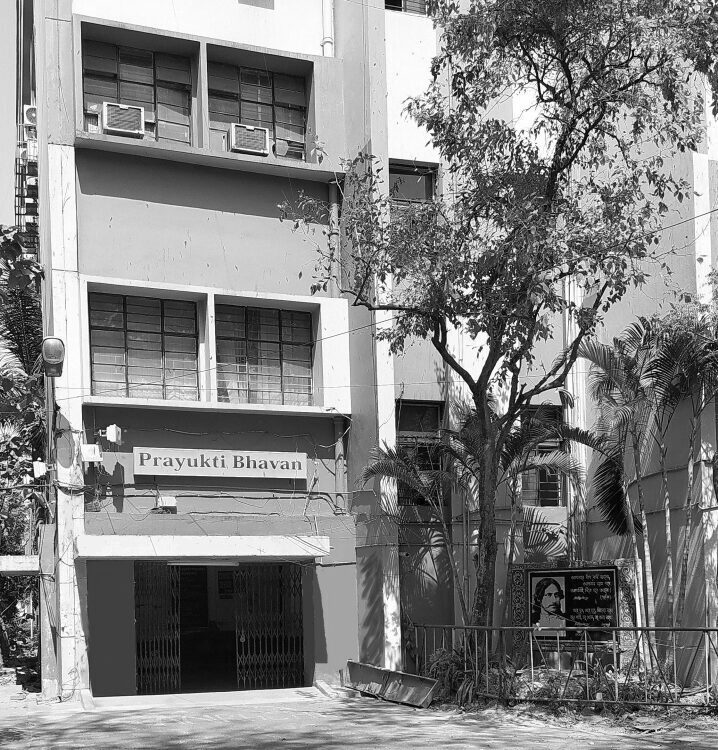
\includegraphics[width=0.3\linewidth]{images/prayukti.jpg}}
  \raisebox{-0.55\height}{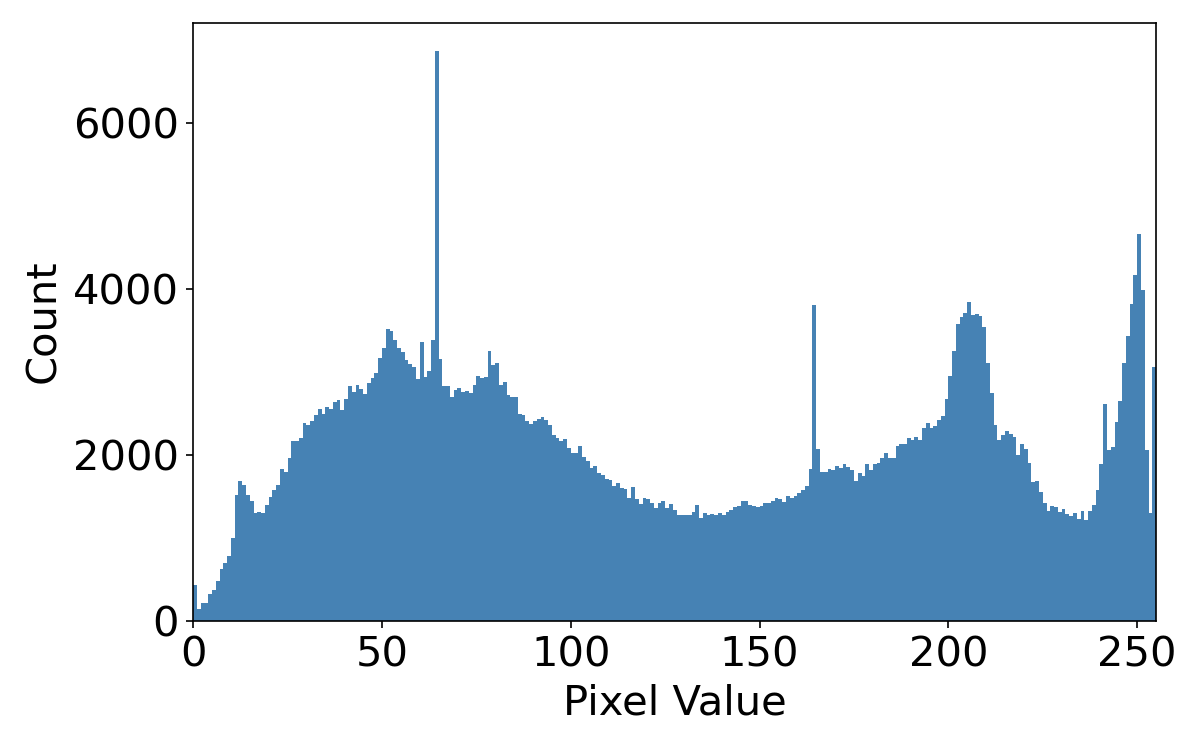
\includegraphics[width=0.6\linewidth]{images/prayukti_histogram.png}}
  \caption{Example image and its histogram}
\end{figure}

\subsection*{Contrast Stretching}

Contrast stretching (normalization) linearly expands an image’s
dynamic range, making low-contrast images more vivid. It’s the
simplest boost, though it can exaggerate noise or outliers.

\begin{equation*}
  s_k = T(r_k)
  = \frac{r_k - r_{\min}}{r_{\max} - r_{\min}}
  \times (L - 1)
\end{equation*}

where: (i) $r_k\rightarrow$ input intensity, (ii) $s_k\rightarrow$
output intensity, (iii) $r_{\min},\,r_{\max}\rightarrow$ observed
minimum and maximum intensities in the image, (iv) $L\rightarrow$
number of possible intensity levels

\begin{algorithm}[ht!]
  \DontPrintSemicolon
  Find $r_{\min}$ and $r_{\max}$ in input image $I$ \;

  {
    Apply T to each pixel intensity $r_k$ in $I$ \;
    \nonl $s_k \leftarrow \bigl(r_k -
    r_{\min}\bigr)\,/\,\bigl(r_{\max}-r_{\min}\bigr)\times(L-1)$ \;
    \nonl where $L$ is the number of intensity levels \;
  }

  Return contrast-stretched image $I'$\;
  \caption{Contrast Stretching}
\end{algorithm}

\subsection*{Histogram Equalization}

Refers to \enquote{spreading out} (equalizing) the frequencies in an
image. Simple way to improve dark or washed out images.

\begin{equation*}
  s_k = T(r_k) = \sum_{j=1}^{k} p_r(r_j) = \sum_{j=1}^{k} \frac{n_j}{n}
\end{equation*}

where: (i) $r_k \rightarrow$ input intensity, (ii) $s_k \rightarrow$
processed intensity, (iii) $k \rightarrow$ intensity range (e.g. 0 -
1), (iv) $n_j \rightarrow$ frequency of intensity $j$, (v) $n
\rightarrow$ total number of pixels (v) $L\rightarrow$ number of
possible intensity levels

\begin{algorithm}[ht!]
  \DontPrintSemicolon
  Compute histogram of input image $I$ \;
  Compute CDF from histogram \;
  Normalize CDF by dividing by $n$ \;

  {
    Apply $T$ to each pixel intensity $r_k$ in $I$\\
    \nonl $s_k = \text{CDF}[r_k] \times (L - 1)$ \\
    \nonl where $L$ is the number of intensity levels \;
  }

  Return enhanced image $I'$\;
  \caption{Histogram Equalization}
\end{algorithm}

\subsection*{Point Processing}

Simplest spatial domain operation, neighborhood is the pixel itself.

\subsubsection*{Negative Images}

Simply inverts pixel values; useful for enhancing dark regions.
\begin{equation*}
  s = (L - 1) - r
\end{equation*}

\subsubsection*{Thresholding}

Segments an image by \textbf{converting it to binary} based on a
threshold value (say $\theta_0$); useful for isolating objects from
the background.

\begin{equation*}
  s =
  \begin{cases}
    0 & \text{if } r < \theta_0 \\
    L - 1 & \text{if } r \geq \theta_0
  \end{cases}
\end{equation*}

\subsubsection*{Gray Level Transforms}

\begin{figure}[H]
  \centering
  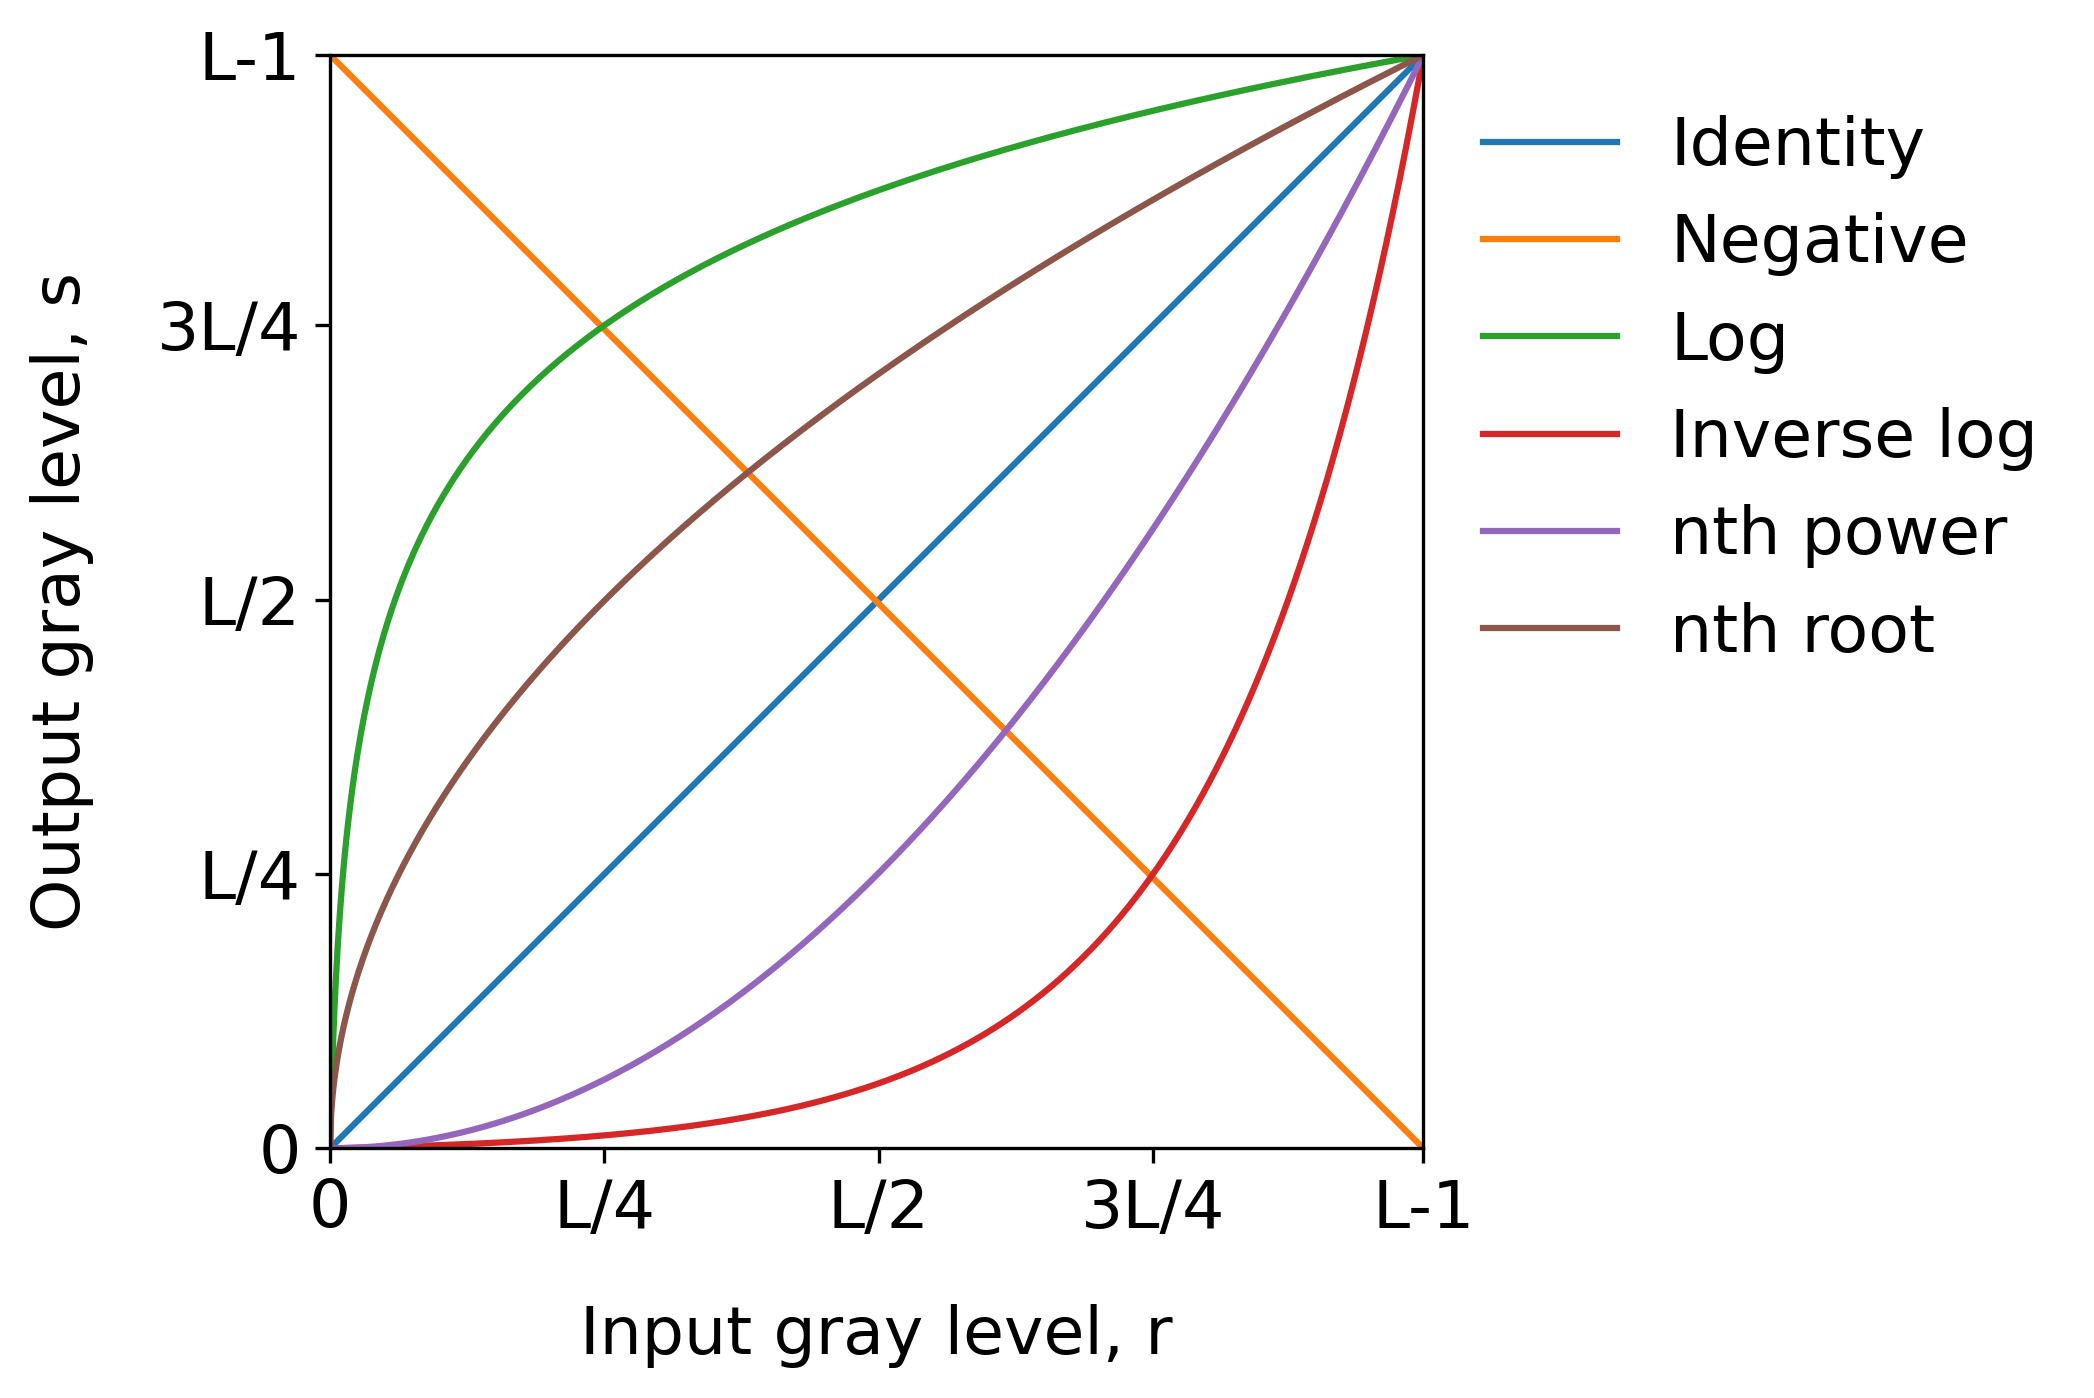
\includegraphics[width=\linewidth]{images/gray_level_transforms.png}
  \caption{Gray level transforms}
\end{figure}

\begin{itemize}
  \item \textbf{Log Transform:} Maps a narrow range of low input grey
    level values into a wider range of output values.
    \begin{itemize}
      \item $s = c \times \log(1 + r)$, where $c$ is a constant
      \item Useful when the input grey level values may have an
        extremely large range of values
      \item Use case 1: \textbf{log transform on Fourier transform}.
        More details are revealed.
      \item Use case 2: \textbf{gamma correction in displays}. Some
        displays do not respond linearly to different intensities;
        can be corrected using log transform
    \end{itemize}

  \item \textbf{Power Law Transform:} Maps a narrow range of dark
    input grey level values into a wider range of output values.
    \begin{itemize}
      \item $s = c \times r^{\gamma}$, where $\gamma$ is a constant
      \item Different $\gamma$ values highlight different details
      \item Useful for enhancing images with high dynamic range
    \end{itemize}

  \item \textbf{Piecewise Linear Transform:} Combines multiple
    arbitrary user-defined linear segments to create a more complex mapping.
    \begin{itemize}
      \item Useful for enhancing specific ranges of pixel values
      \item Can be used to adjust contrast in specific regions of an image
    \end{itemize}

    \begin{minipage}{\linewidth}
      \vspace{-0.5cm}
      \begin{figure}[H]
        \centering
        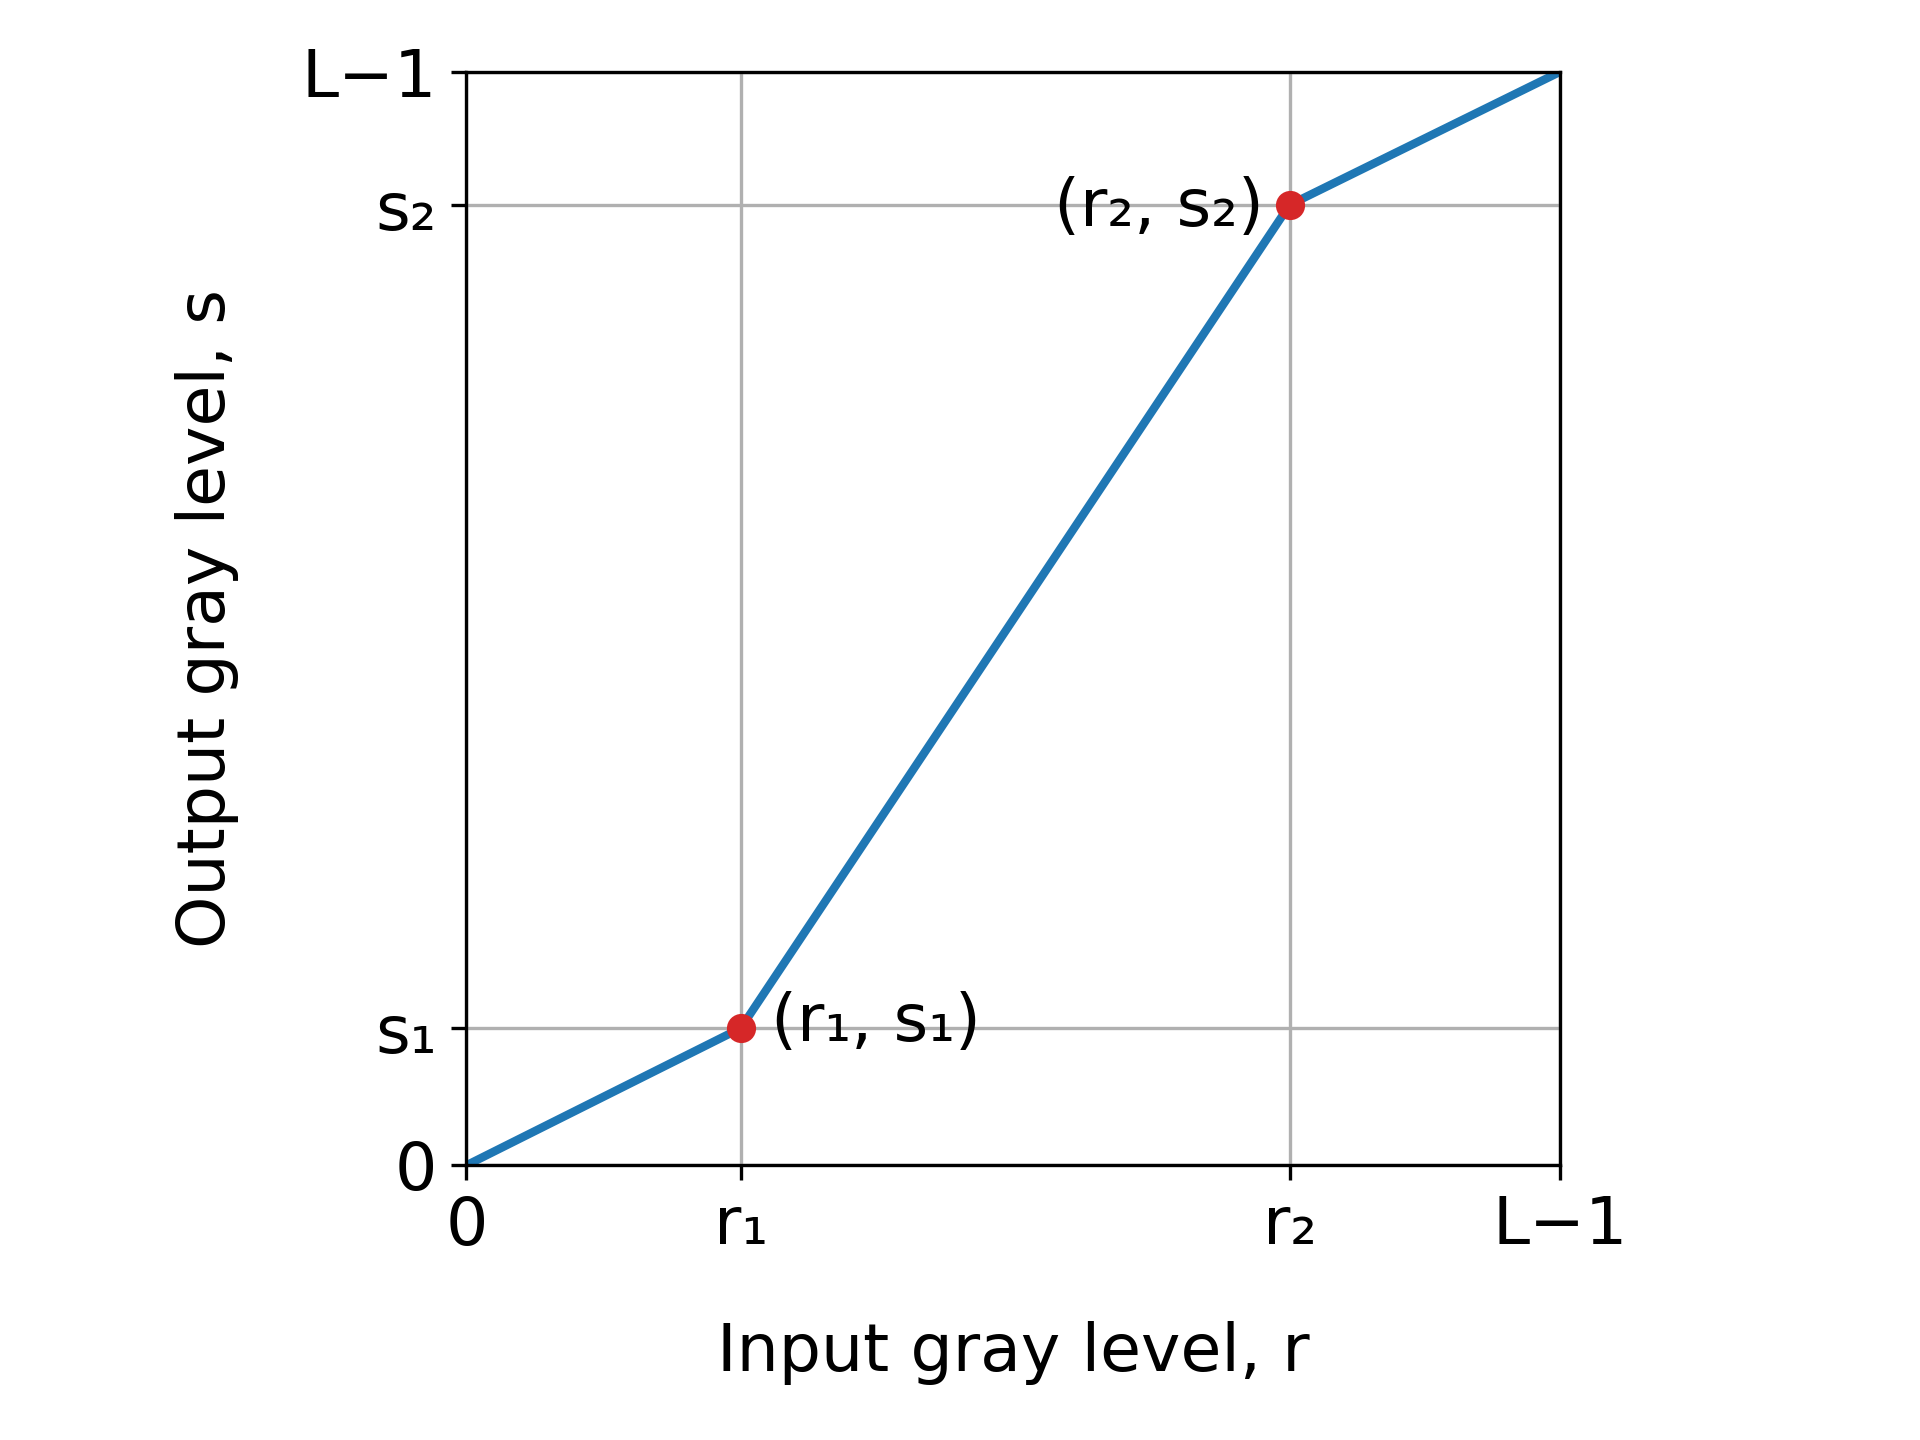
\includegraphics[width=\linewidth]{images/piecewise_transform.png}
        \vspace{-0.5cm}
        \caption{Piecewise linear transform}
      \end{figure}
    \end{minipage}

  \item \textbf{Gray Level Slicing:} Similar to thresholding, but
    allows for a range of pixel values to be highlighted.
    \begin{itemize}
      \item Other levels can be suppressed or maintained
      \item Useful for enhancing specific features in an image
    \end{itemize}

    \begin{minipage}{\linewidth}
      \begin{figure}[H]
        \centering
        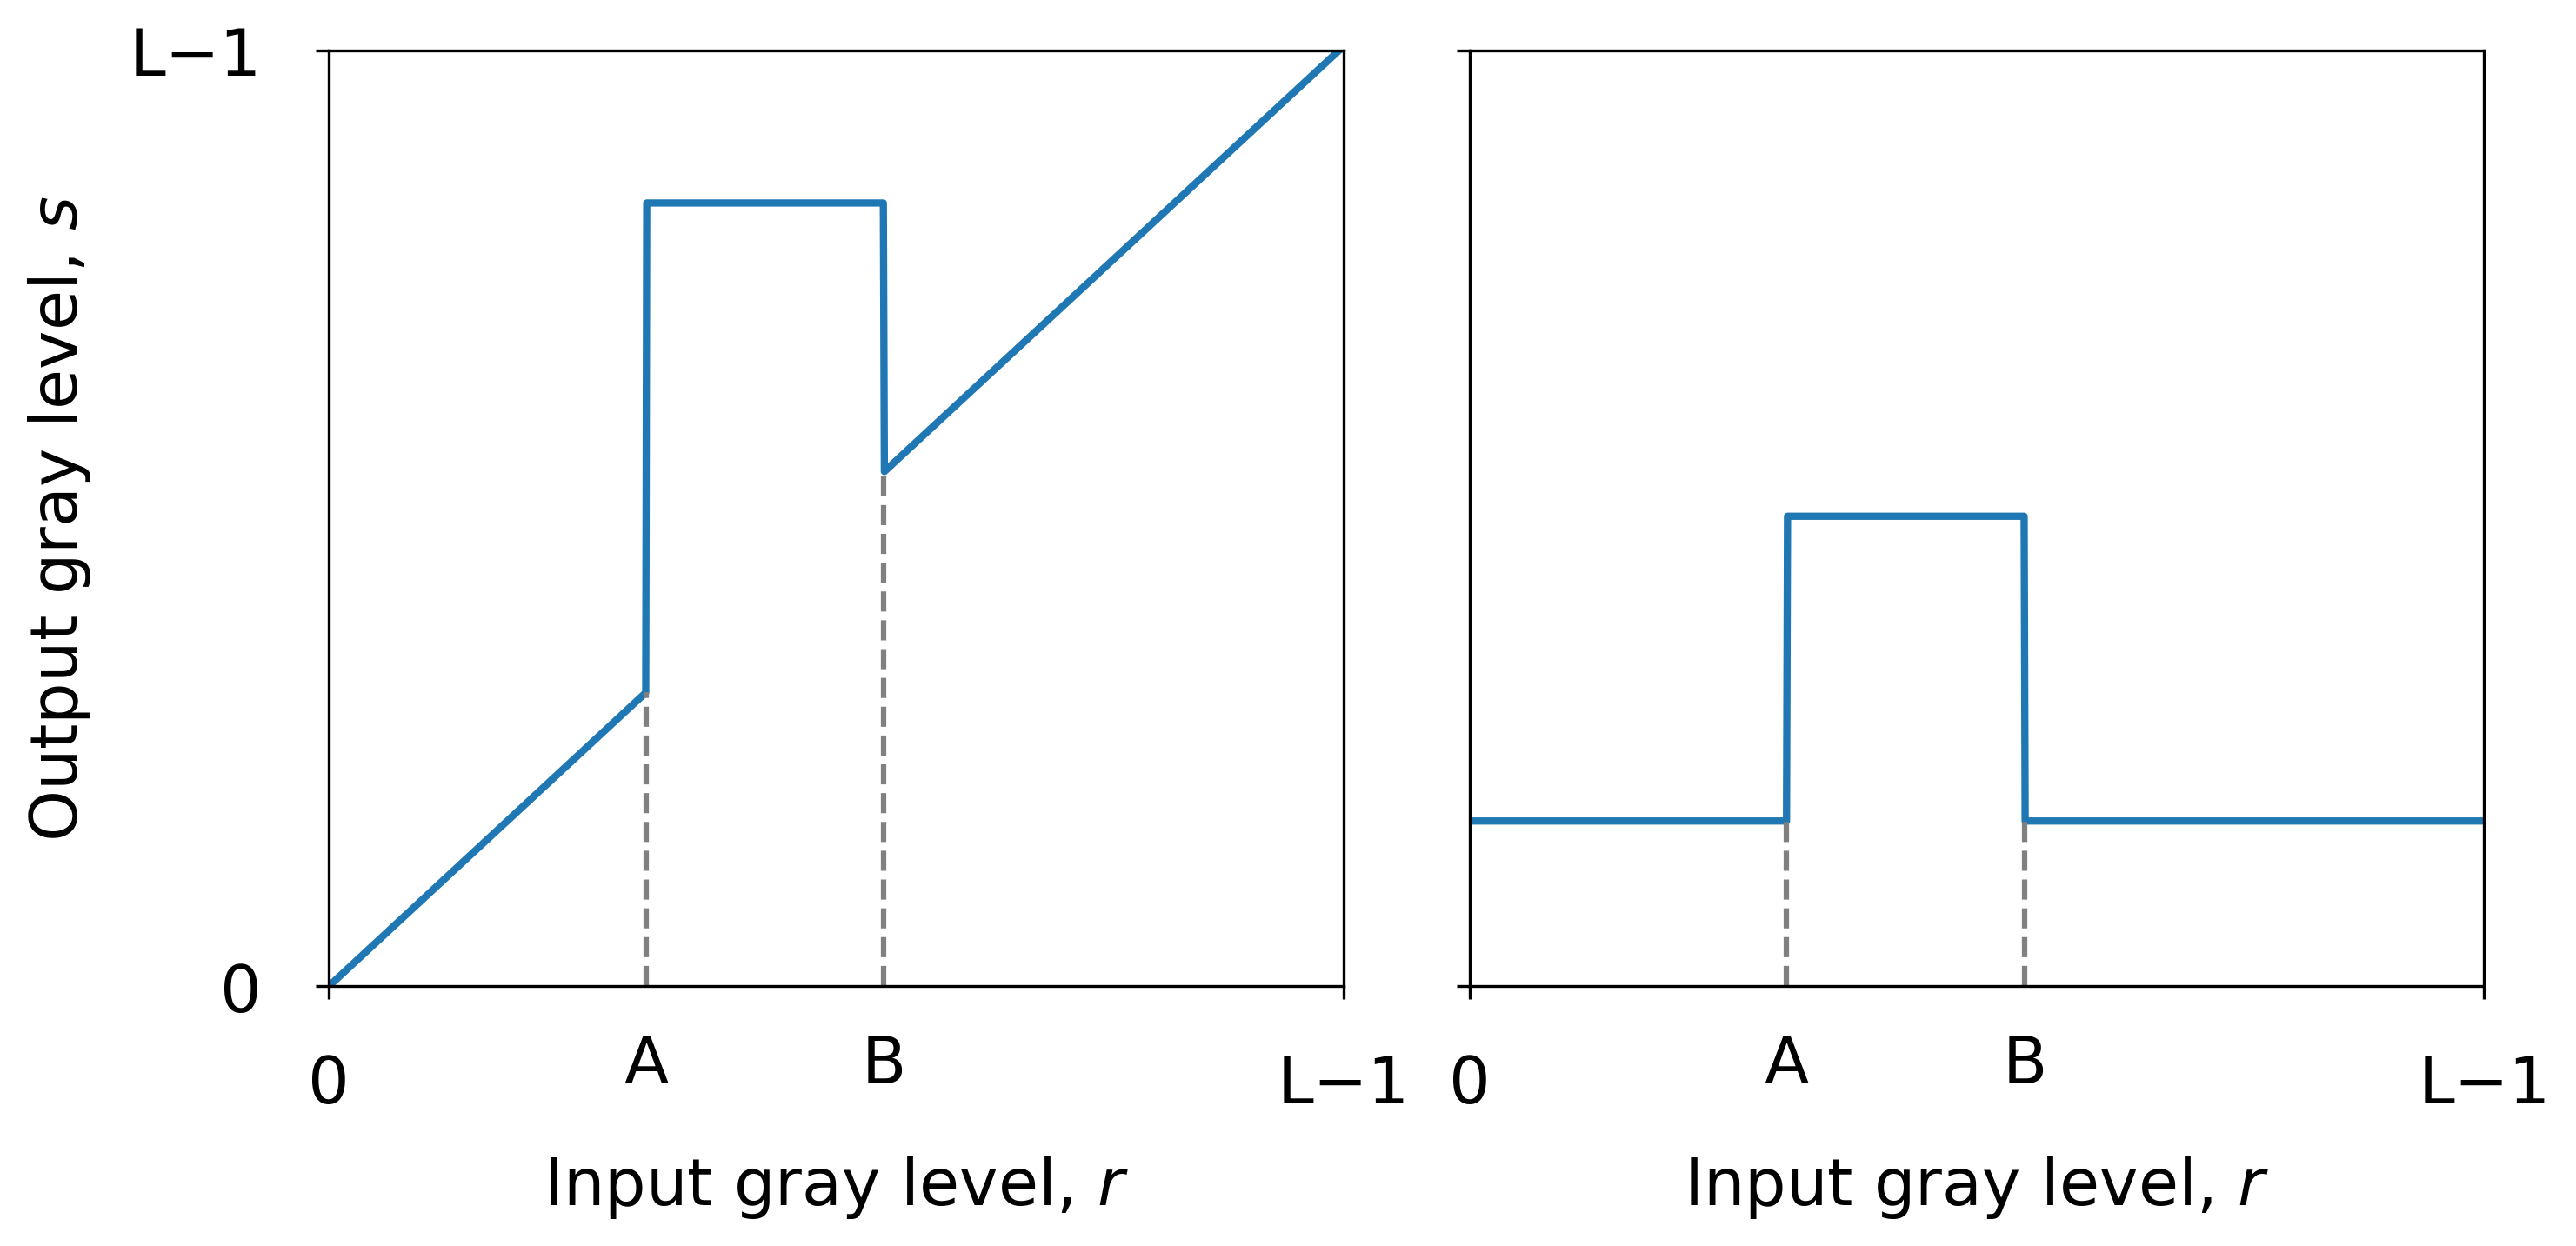
\includegraphics[width=\linewidth]{images/gray_level_slicing.png}
        \caption{Gray level slicing with (i) background retained (ii)
        background supressed}
      \end{figure}
    \end{minipage}

  \item \textbf{Bit-Plane Slicing:} By isolating particular bits of
    the pixel values in an image, we can highligh interesting aspects
    of that image.
    \begin{itemize}
      \item Higher order bits contain most of the significant information
      \item Lower order bits contain subtle details
      \item \enquote{Bit planes} are arranged in a stack; MSB at the
        top, LSB at the bottom.
    \end{itemize}

    \begin{minipage}{\linewidth}
      \begin{figure}[H]
        \centering
        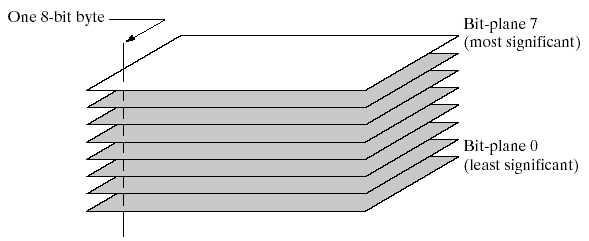
\includegraphics[width=\linewidth]{images/bit_plane_slicing.png}
        \caption{Bit-plane slicing of an 8-bit image}
      \end{figure}
      \vspace{-0.5cm}
    \end{minipage}

\end{itemize}

\subsection*{Neighborhood Operations}

Operations on a \textbf{rectangular region} around a pixel. Any size
rectangle and any shape filter are possible.

\subsubsection*{Simple Neighborhood Operations}

For any pixel $p$ in an image at the center of a neighborhood:

\begin{itemize}
  \item \textbf{Min:} Sets $p$ to minimum value in the neighborhood.
    \begin{itemize}
        \vspace{-0.2cm}
      \item Removes small bright spots (\textbf{salt noise})
      \item Makes \textbf{dark regions darker}
    \end{itemize}
  \item \textbf{Max:} Sets $p$ to maximum value in the neighborhood.
    \begin{itemize}
        \vspace{-0.2cm}
      \item Removes small dark spots (\textbf{pepper noise})
      \item Makes \textbf{bright regions brighter}
    \end{itemize}
  \item \textbf{Median:} Sets $p$ to median value in the neighborhood.
    \begin{itemize}
        \vspace{-0.2cm}
      \item Removes \textbf{salt and pepper noise}
    \end{itemize}
\end{itemize}

\subsubsection*{Spatial Differentiation}

Differentiation measures the \textit{rate of change} of a function.
In the context of image processing, the function is the pixel
intensity, and differentiation helps identify edges and transitions
in the image.

\begin{itemize}
  \item \textbf{First Derivative:} Measures the rate of change of
    pixel intensity.
    \begin{gather*}
      \frac{\partial f}{\partial x} = f(x + 1, y) - f(x, y)\\
      \frac{\partial f}{\partial y} = f(x, y + 1) - f(x, y)
    \end{gather*}
  \item \textbf{Second Derivative:} Measures the rate of change of
    the first derivative.
    \begin{gather*}
      \frac{\partial^2 f}{\partial x^2} = f(x + 1, y) + f(x - 1, y) - 2f(x, y)\\
      \frac{\partial^2 f}{\partial y^2} = f(x, y + 1) + f(x, y - 1) - 2f(x, y)
    \end{gather*}
  \item \textbf{The Laplacian:} Combines the second derivatives in
    both x and y directions.
    \begin{equation*}
      \nabla^2 f = \frac{\partial^2 f}{\partial x^2} +
      \frac{\partial^2 f}{\partial y^2}
    \end{equation*}
    In practice, the Laplacian is applied using a \textbf{filter}.
\end{itemize}

\begin{tblr}{
    colspec={@{}l X[l] | X[l]},
    row{1} = {c, font=\bfseries},
  }
  \cline{2-3}
  & \textbf{First Derivative} & \textbf{Second Derivative} \\
  \cline{2-3}
  \textbullet & Generally produces thicker edges
  & Stronger response to fine detail (e.g.\ thin lines) \\[6pt]
  \textbullet & Stronger response to grey level step
  & Double response to step changes in grey level \\[6pt]
\end{tblr}

\subsubsection*{Correlation vs Convolution}

Most spatial filtering operations are technically
\textbf{correlation}, and the filter is referred to as a
\textbf{correlation kernel} or \textbf{mask}. \textbf{Convolution} is
a similar operation, with a subtle difference:

\begin{figure}[H]
  \centering
  \begin{tikzpicture}[%
      imgcell/.style={draw=black, fill=white, minimum size=1cm, anchor=center},
      filtercell/.style={draw=MaterialBlue900, fill=MaterialBlue50,
      minimum size=1cm, anchor=center}
    ]

    % Original image grid
    \node[imgcell] (i11) at (0,2) {$r_1$};
    \node[imgcell] (i12) at (1,2) {$r_2$};
    \node[imgcell] (i13) at (2,2) {$r_3$};
    \node[imgcell] (i21) at (0,1) {$r_4$};
    \node[imgcell, fill=MaterialGrey200] (i22) at (1,1) {$r_5$};
    \node[imgcell] (i23) at (2,1) {$r_6$};
    \node[imgcell] (i31) at (0,0) {$r_7$};
    \node[imgcell] (i32) at (1,0) {$r_8$};
    \node[imgcell] (i33) at (2,0) {$r_9$};

    % Convolution symbol
    \node at (3,1) {\large $\ast$};

    % Filter grid
    \node[filtercell] (f11) at (4,2) {$k_1$};
    \node[filtercell] (f12) at (5,2) {$k_2$};
    \node[filtercell] (f13) at (6,2) {$k_3$};
    \node[filtercell] (f21) at (4,1) {$k_4$};
    \node[filtercell] (f22) at (5,1) {$k_5$};
    \node[filtercell] (f23) at (6,1) {$k_6$};
    \node[filtercell] (f31) at (4,0) {$k_7$};
    \node[filtercell] (f32) at (5,0) {$k_8$};
    \node[filtercell] (f33) at (6,0) {$k_9$};

  \end{tikzpicture}
  \caption{An image (left) being operated on by a filter (right). The
    result depends
  on whether the operation is correlation or convolution.}
\end{figure}
\vspace{-0.5cm}
\begin{itemize}
  \item \textbf{Correlation:} The filter is applied directly to the
    image, without flipping it.
    \vspace{-0.2cm}
    \begin{equation*}
      s = r_1 k_1 + r_2 k_2 + r_3 k_3 + r_4 k_4 + r_5 k_5 + r_6 k_6 +
      r_7 k_7 + r_8 k_8 + r_9 k_9\\[-0.3cm]
    \end{equation*}
  \item \textbf{Convolution:} The filter is flipped both horizontally
    and vertically before being applied to the image.
    \vspace{-0.2cm}
    \begin{equation*}
      s = r_1 k_9 + r_2 k_8 + r_3 k_7 + r_4 k_6 + r_5 k_5 + r_6 k_4 +
      r_7 k_3 + r_8 k_2 + r_9 k_1\\[-0.3cm]
    \end{equation*}
\end{itemize}

\subsubsection*{Handling Boundary Effects}

Edge pixels don't have a full neighborhood. A filter applied on a
pixel on or near the image boundaries \textbf{may exceed the image
boundaries}, leading to undefined behavior. There are strategies to
handle this:

\begin{minipage}{\linewidth}
  \begin{figure}[H]
    \centering
    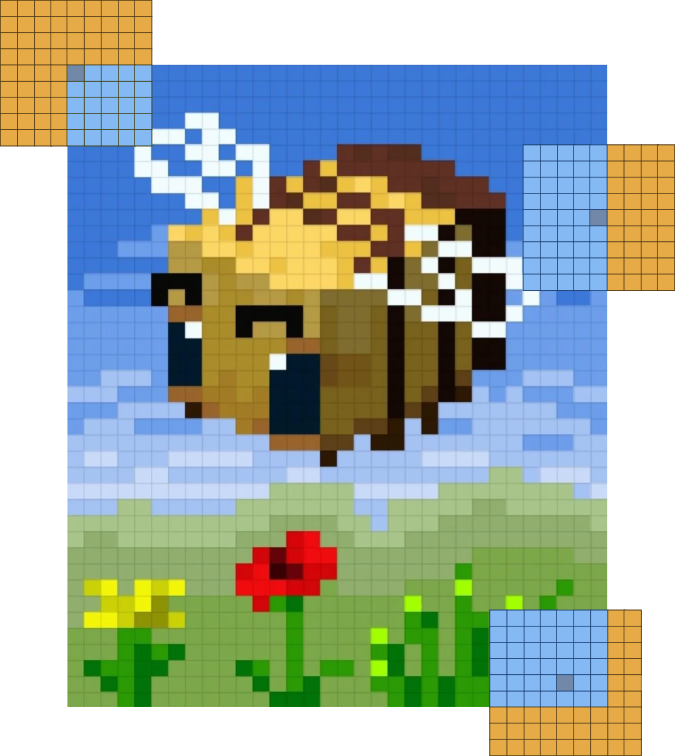
\includegraphics[width=0.6\linewidth]{images/edges.png}
    \caption{A filter may exceed the image boundaries}
  \end{figure}
\end{minipage}

\begin{itemize}
  \item \textbf{Valid (Crop)}: Only compute outputs where the kernel
    lies entirely inside; reduces output size.
  \item \textbf{Partial (Truncate)}: Ignore kernel weights falling
    outside and renormalize the remainder; minor overhead.
  \item \textbf{Constant Pad}: Add a border of fixed-value pixels
    (e.g.\ zero or white) to restore full output dimensions.
  \item \textbf{Replicate}: Extend the nearest edge pixel values
    outward; simple and fast, with minimal artifacts.
  \item \textbf{Reflect}: Mirror the image at its borders; preserves
    continuity but may introduce mirrored features.
\end{itemize}

\subsubsection*{Linear Spatial Filters}

\begin{equation*}
  g(x, y) = \sum_{s=-a}^{a} \sum_{t=-b}^{b} w(s, t) f(x + s, y + t)
\end{equation*}

\begin{itemize}
  \item \textbf{Identity Filter:} Leaves the image unchanged. Simply
    assigns a weight \enquote{0} to all the neighbors around the central pixel.

    \begin{minipage}{\linewidth}
      \vspace{-0.3cm}
      \begin{figure}[H]
        \centering
        \begin{tikzpicture}[%
            filtercell/.style={draw=MaterialBlue900, fill=MaterialBlue50,
            minimum size=1cm, anchor=center}
          ]
          \node[filtercell] (f11) at (0,2) {$0$};
          \node[filtercell] (f12) at (1,2) {$0$};
          \node[filtercell] (f13) at (2,2) {$0$};
          \node[filtercell] (f21) at (0,1) {$0$};
          \node[filtercell] (f22) at (1,1) {$1$};
          \node[filtercell] (f23) at (2,1) {$0$};
          \node[filtercell] (f31) at (0,0) {$0$};
          \node[filtercell] (f32) at (1,0) {$0$};
          \node[filtercell] (f33) at (2,0) {$0$};

        \end{tikzpicture}
        \caption{Identity filter}
      \end{figure}
    \end{minipage}
  \item \textbf{Smoothing Filters:} Smooths an image by averaging
    pixel values in the neighborhood.
    \begin{itemize}
      \item \textbf{Mean filter} or \textbf{simple
        averaging filter}: simplest form; $k \times k$ matrix, each
        element is $1/k^2$.

        \begin{minipage}{\linewidth}
          \vspace{-0.3cm}
          \begin{figure}[H]
            \centering
            \begin{tikzpicture}[%
                filtercell/.style={draw=MaterialBlue900, fill=MaterialBlue50,
                minimum size=1cm, anchor=center}
              ]
              \node[filtercell] (f11) at (0,2) {$1/9$};
              \node[filtercell] (f12) at (1,2) {$1/9$};
              \node[filtercell] (f13) at (2,2) {$1/9$};
              \node[filtercell] (f21) at (0,1) {$1/9$};
              \node[filtercell] (f22) at (1,1) {$1/9$};
              \node[filtercell] (f23) at (2,1) {$1/9$};
              \node[filtercell] (f31) at (0,0) {$1/9$};
              \node[filtercell] (f32) at (1,0) {$1/9$};
              \node[filtercell] (f33) at (2,0) {$1/9$};

            \end{tikzpicture}
            \caption{Simple 3x3 averaging filter}
          \end{figure}
        \end{minipage}
      \item \textbf{Weighted averaging filter}: Sometimes different
        pixels in the neighborhood are weighted differently; the
        filter values always add up to 1.

        \begin{minipage}{\linewidth}
          \vspace{-0.3cm}
          \begin{figure}[H]
            \centering
            \begin{tikzpicture}[%
                filtercell/.style={draw=MaterialBlue900, fill=MaterialBlue50,
                minimum size=1cm, anchor=center}
              ]
              \node[filtercell] (f11) at (0,2) {$1/16$};
              \node[filtercell] (f12) at (1,2) {$2/16$};
              \node[filtercell] (f13) at (2,2) {$1/16$};
              \node[filtercell] (f21) at (0,1) {$2/16$};
              \node[filtercell] (f22) at (1,1) {$4/16$};
              \node[filtercell] (f23) at (2,1) {$2/16$};
              \node[filtercell] (f31) at (0,0) {$1/16$};
              \node[filtercell] (f32) at (1,0) {$2/16$};
              \node[filtercell] (f33) at (2,0) {$1/16$};

            \end{tikzpicture}
            \caption{Weighted 3x3 averaging filter}
          \end{figure}
        \end{minipage}

      \item \textbf{Useful for}: (i) removing noise from images (ii)
        highlighting gross details
    \end{itemize}
  \item \textbf{Sharpening Filters:} Enhances edges, removes blurring
    and fine details in an image.
    \begin{itemize}
      \item \textbf{Laplacian Filter:} Highlights regions of rapid
        intensity change (edges and other discontinuities).
        \begin{itemize}
          \item The Laplacian output is \textbf{not an enhanced
            image}; it is an image with those regions highlighted,
            where the pixel values change rapidly in the original
            image (edges etc.)
          \item In order to obtain the enhanced image, the Laplacian
            output is \textbf{subtracted} from the original image.
          \item This above operation can be summarized as a new
            filter: identity minus Laplacian.
        \end{itemize}

        \begin{minipage}{\linewidth}
          \vspace{-0.3cm}
          \begin{figure}[H]
            \centering
            \begin{tikzpicture}[%
                filtercell/.style={draw=MaterialBlue900, fill=MaterialBlue50,
                minimum size=1cm, anchor=center}
              ]
              \node[filtercell] (f111) at (0,2) {$0$};
              \node[filtercell] (f112) at (1,2) {$1$};
              \node[filtercell] (f113) at (2,2) {$0$};
              \node[filtercell] (f121) at (0,1) {$1$};
              \node[filtercell] (f122) at (1,1) {$4$};
              \node[filtercell] (f123) at (2,1) {$1$};
              \node[filtercell] (f131) at (0,0) {$0$};
              \node[filtercell] (f132) at (1,0) {$1$};
              \node[filtercell] (f133) at (2,0) {$0$};

              \node[filtercell] (f211) at (4,2) {$0$};
              \node[filtercell] (f212) at (5,2) {$-1$};
              \node[filtercell] (f213) at (6,2) {$0$};
              \node[filtercell] (f221) at (4,1) {$-1$};
              \node[filtercell] (f222) at (5,1) {$5$};
              \node[filtercell] (f223) at (6,1) {$-1$};
              \node[filtercell] (f231) at (4,0) {$0$};
              \node[filtercell] (f232) at (5,0) {$-1$};
              \node[filtercell] (f233) at (6,0) {$0$};
            \end{tikzpicture}
            \caption{Laplacian filter (left), Identity minus
            Laplacian filter (right)}
          \end{figure}
        \end{minipage}

      \item \textbf{Unsharp Mask and High-Boost Filtering:} These are
        filters that enhance edges by subtracting a blurred version
        of the image ($\bar{f}(x, y)$) from the original image ($f(x, y)$)
        \begin{gather*}
          f_\textnormal{s}(x, y) = f(x, y) - \bar{f}(x, y)\\
          f_\textnormal{hb}(x, y) = Af(x, y) - \bar{f}(x, y)
        \end{gather*}
        \begin{itemize}
          \item High-boost filtering ($f_\textnormal{hb}$) takes a
            strength parameter $A$. Unsharp mask ($f_\textnormal{s}$)
            is a special case of high-boost filtering with $A = 1$.
        \end{itemize}
    \end{itemize}
    \begin{minipage}{\linewidth}
      \vspace{-0.3cm}
      \begin{figure}[H]
        \centering
        \begin{tikzpicture}[%
            filtercell/.style={draw=MaterialBlue900, fill=MaterialBlue50,
            minimum size=1cm, anchor=center}
          ]
          \node[filtercell] (f111) at (0,2) {$0$};
          \node[filtercell] (f112) at (1,2) {$-1$};
          \node[filtercell] (f113) at (2,2) {$0$};
          \node[filtercell] (f121) at (0,1) {$-1$};
          \node[filtercell] (f122) at (1,1) {\small \hspace{-0.5em} $A + 4$};
          \node[filtercell] (f123) at (2,1) {$-1$};
          \node[filtercell] (f131) at (0,0) {$0$};
          \node[filtercell] (f132) at (1,0) {$-1$};
          \node[filtercell] (f133) at (2,0) {$0$};

          \node[filtercell] (f211) at (4,2) {$-1$};
          \node[filtercell] (f212) at (5,2) {$-1$};
          \node[filtercell] (f213) at (6,2) {$-1$};
          \node[filtercell] (f221) at (4,1) {$-1$};
          \node[filtercell] (f222) at (5,1) {\small \hspace{-0.5em} $A + 8$};
          \node[filtercell] (f223) at (6,1) {$-1$};
          \node[filtercell] (f231) at (4,0) {$-1$};
          \node[filtercell] (f232) at (5,0) {$-1$};
          \node[filtercell] (f233) at (6,0) {$-1$};
        \end{tikzpicture}
        \caption{Two forms of unsharp mask}
      \end{figure}
    \end{minipage}

    For the specific case of a 3x3 filter, the unsharp mask perfectly
    matches the \enquote{identity minus Laplacian filter}!

  \item \textbf{Sobel Filters:} Based on 1st derivative filtering,
    these are typically used for edge detection.
    \begin{itemize}
      \item The Sobel filters are based on the calculation of
        gradients in the x and y directions. As such, there are two
        filters, one for $G_x$ and one for $G_y$.
      \item To filter an image, (i) both the filters are applied and
        (ii) the results are added together.
    \end{itemize}

    \begin{minipage}{\linewidth}
      \vspace{-0.3cm}
      \begin{figure}[H]
        \centering
        \begin{tikzpicture}[%
            filtercell/.style={draw=MaterialBlue900, fill=MaterialBlue50,
            minimum size=1cm, anchor=center}
          ]
          \node[filtercell] (f111) at (0,2) {$-1$};
          \node[filtercell] (f112) at (1,2) {$0$};
          \node[filtercell] (f113) at (2,2) {$1$};
          \node[filtercell] (f121) at (0,1) {$-2$};
          \node[filtercell] (f122) at (1,1) {$0$};
          \node[filtercell] (f123) at (2,1) {$2$};
          \node[filtercell] (f131) at (0,0) {$-1$};
          \node[filtercell] (f132) at (1,0) {$0$};
          \node[filtercell] (f133) at (2,0) {$1$};

          \node[filtercell] (f211) at (4,2) {$-1$};
          \node[filtercell] (f212) at (5,2) {$-2$};
          \node[filtercell] (f213) at (6,2) {$-1$};
          \node[filtercell] (f221) at (4,1) {$0$};
          \node[filtercell] (f222) at (5,1) {$0$};
          \node[filtercell] (f223) at (6,1) {$0$};
          \node[filtercell] (f231) at (4,0) {$1$};
          \node[filtercell] (f232) at (5,0) {$2$};
          \node[filtercell] (f233) at (6,0) {$1$};
        \end{tikzpicture}
        \caption{The Sobel filters for $G_x$/horizontal derivative
        (left) and $G_y$/vertical derivative (right)}
      \end{figure}
    \end{minipage}
\end{itemize}

\section*{Spatial Domain Enhancement}

\subsection*{Image Histogram}

Shows the \textbf{distribution of pixel intensities} in an image.
Massively useful, especially for segmentation.

\begin{figure}[H]
  \centering
  \raisebox{-0.5\height}{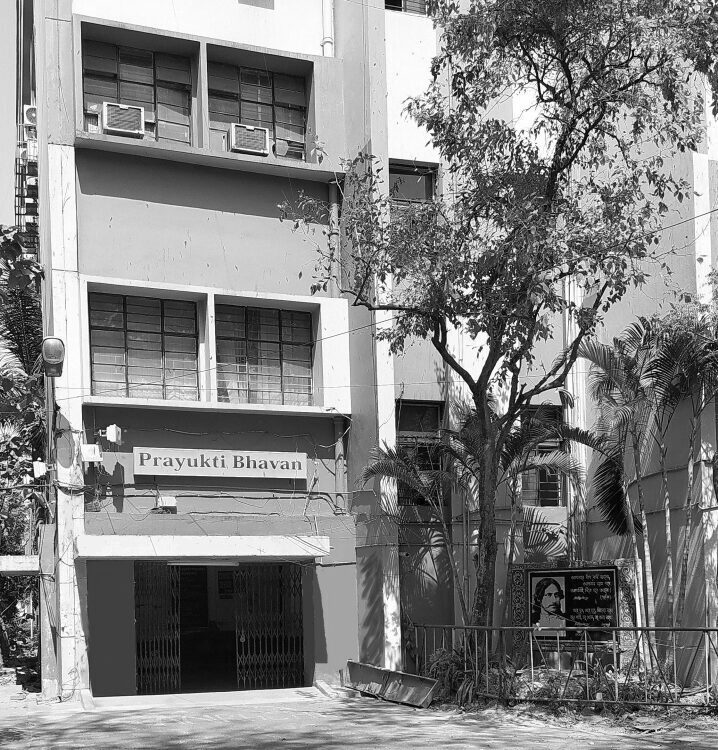
\includegraphics[width=0.3\linewidth]{images/prayukti.jpg}}
  \raisebox{-0.55\height}{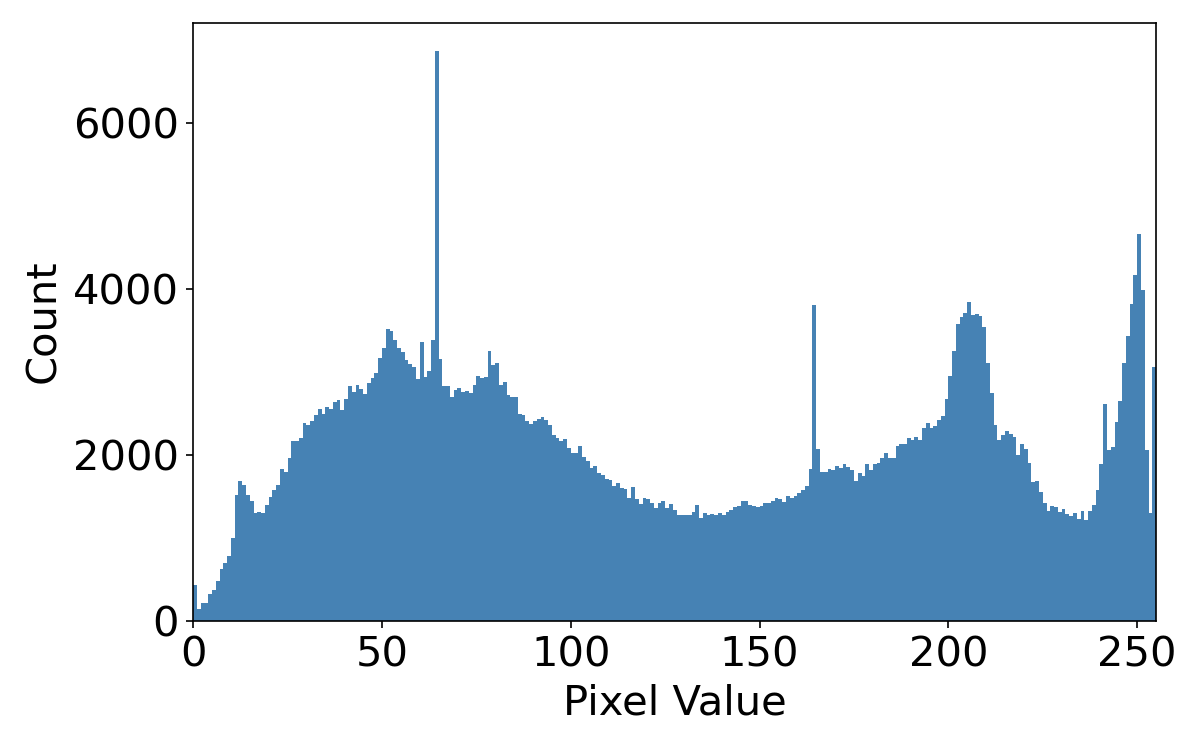
\includegraphics[width=0.6\linewidth]{images/prayukti_histogram.png}}
  \caption{Example image and its histogram}
\end{figure}

\subsection*{Contrast Stretching}

Contrast stretching (normalization) linearly expands an image’s
dynamic range, making low-contrast images more vivid. It’s the
simplest boost, though it can exaggerate noise or outliers.

\begin{equation*}
  s_k = T(r_k)
  = \frac{r_k - r_{\min}}{r_{\max} - r_{\min}}
  \times (L - 1)
\end{equation*}

where: (i) $r_k\rightarrow$ input intensity, (ii) $s_k\rightarrow$
output intensity, (iii) $r_{\min},\,r_{\max}\rightarrow$ observed
minimum and maximum intensities in the image, (iv) $L\rightarrow$
number of possible intensity levels

\begin{algorithm}[ht!]
  \DontPrintSemicolon
  Find $r_{\min}$ and $r_{\max}$ in input image $I$ \;

  {
    Apply T to each pixel intensity $r_k$ in $I$ \;
    \nonl $s_k \leftarrow \bigl(r_k -
    r_{\min}\bigr)\,/\,\bigl(r_{\max}-r_{\min}\bigr)\times(L-1)$ \;
    \nonl where $L$ is the number of intensity levels \;
  }

  Return contrast-stretched image $I'$\;
  \caption{Contrast Stretching}
\end{algorithm}

\subsection*{Histogram Equalization}

Refers to \enquote{spreading out} (equalizing) the frequencies in an
image. Simple way to improve dark or washed out images.

\begin{equation*}
  s_k = T(r_k) = \sum_{j=1}^{k} p_r(r_j) = \sum_{j=1}^{k} \frac{n_j}{n}
\end{equation*}

where: (i) $r_k \rightarrow$ input intensity, (ii) $s_k \rightarrow$
processed intensity, (iii) $k \rightarrow$ intensity range (e.g. 0 -
1), (iv) $n_j \rightarrow$ frequency of intensity $j$, (v) $n
\rightarrow$ total number of pixels (v) $L\rightarrow$ number of
possible intensity levels

\begin{algorithm}[ht!]
  \DontPrintSemicolon
  Compute histogram of input image $I$ \;
  Compute CDF from histogram \;
  Normalize CDF by dividing by $n$ \;

  {
    Apply $T$ to each pixel intensity $r_k$ in $I$\\
    \nonl $s_k = \text{CDF}[r_k] \times (L - 1)$ \\
    \nonl where $L$ is the number of intensity levels \;
  }

  Return enhanced image $I'$\;
  \caption{Histogram Equalization}
\end{algorithm}

\subsection*{Point Processing}

Simplest spatial domain operation, neighborhood is the pixel itself.

\subsubsection*{Negative Images}

Simply inverts pixel values; useful for enhancing dark regions.
\begin{equation*}
  s = (L - 1) - r
\end{equation*}

\subsubsection*{Thresholding}

Segments an image by \textbf{converting it to binary} based on a
threshold value (say $\theta_0$); useful for isolating objects from
the background.

\begin{equation*}
  s =
  \begin{cases}
    0 & \text{if } r < \theta_0 \\
    L - 1 & \text{if } r \geq \theta_0
  \end{cases}
\end{equation*}

\subsubsection*{Gray Level Transforms}

\begin{figure}[H]
  \centering
  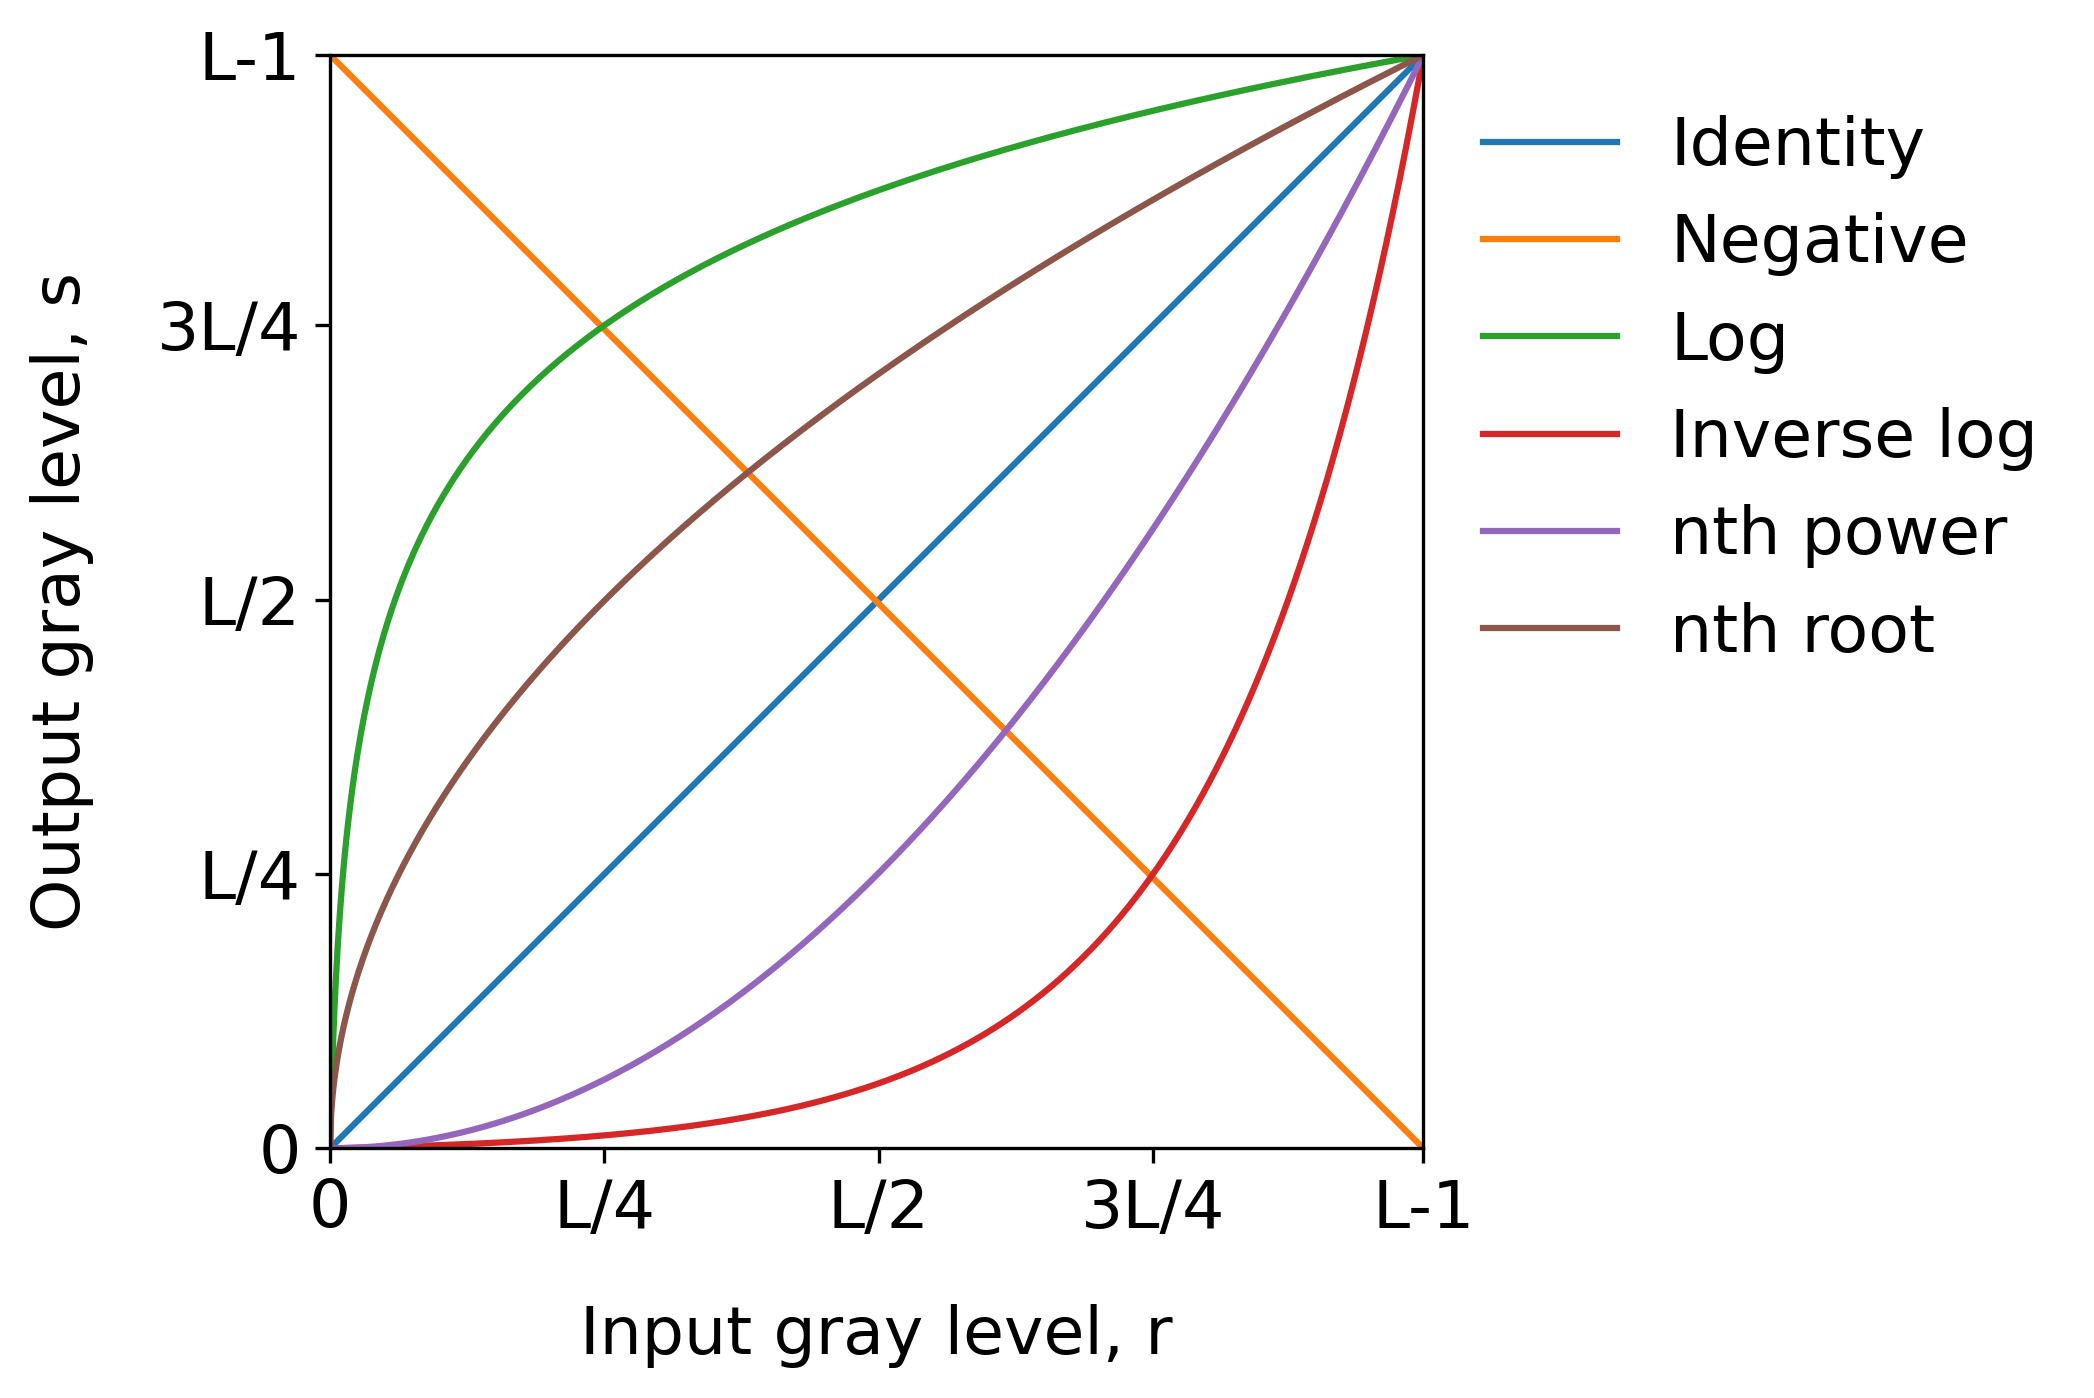
\includegraphics[width=\linewidth]{images/gray_level_transforms.png}
  \caption{Gray level transforms}
\end{figure}

\begin{itemize}
  \item \textbf{Log Transform:} Maps a narrow range of low input grey
    level values into a wider range of output values.
    \begin{itemize}
      \item $s = c \times \log(1 + r)$, where $c$ is a constant
      \item Useful when the input grey level values may have an
        extremely large range of values
      \item Use case 1: \textbf{log transform on Fourier transform}.
        More details are revealed.
      \item Use case 2: \textbf{gamma correction in displays}. Some
        displays do not respond linearly to different intensities;
        can be corrected using log transform
    \end{itemize}

  \item \textbf{Power Law Transform:} Maps a narrow range of dark
    input grey level values into a wider range of output values.
    \begin{itemize}
      \item $s = c \times r^{\gamma}$, where $\gamma$ is a constant
      \item Different $\gamma$ values highlight different details
      \item Useful for enhancing images with high dynamic range
    \end{itemize}

  \item \textbf{Piecewise Linear Transform:} Combines multiple
    arbitrary user-defined linear segments to create a more complex mapping.
    \begin{itemize}
      \item Useful for enhancing specific ranges of pixel values
      \item Can be used to adjust contrast in specific regions of an image
    \end{itemize}

    \begin{minipage}{\linewidth}
      \vspace{-0.5cm}
      \begin{figure}[H]
        \centering
        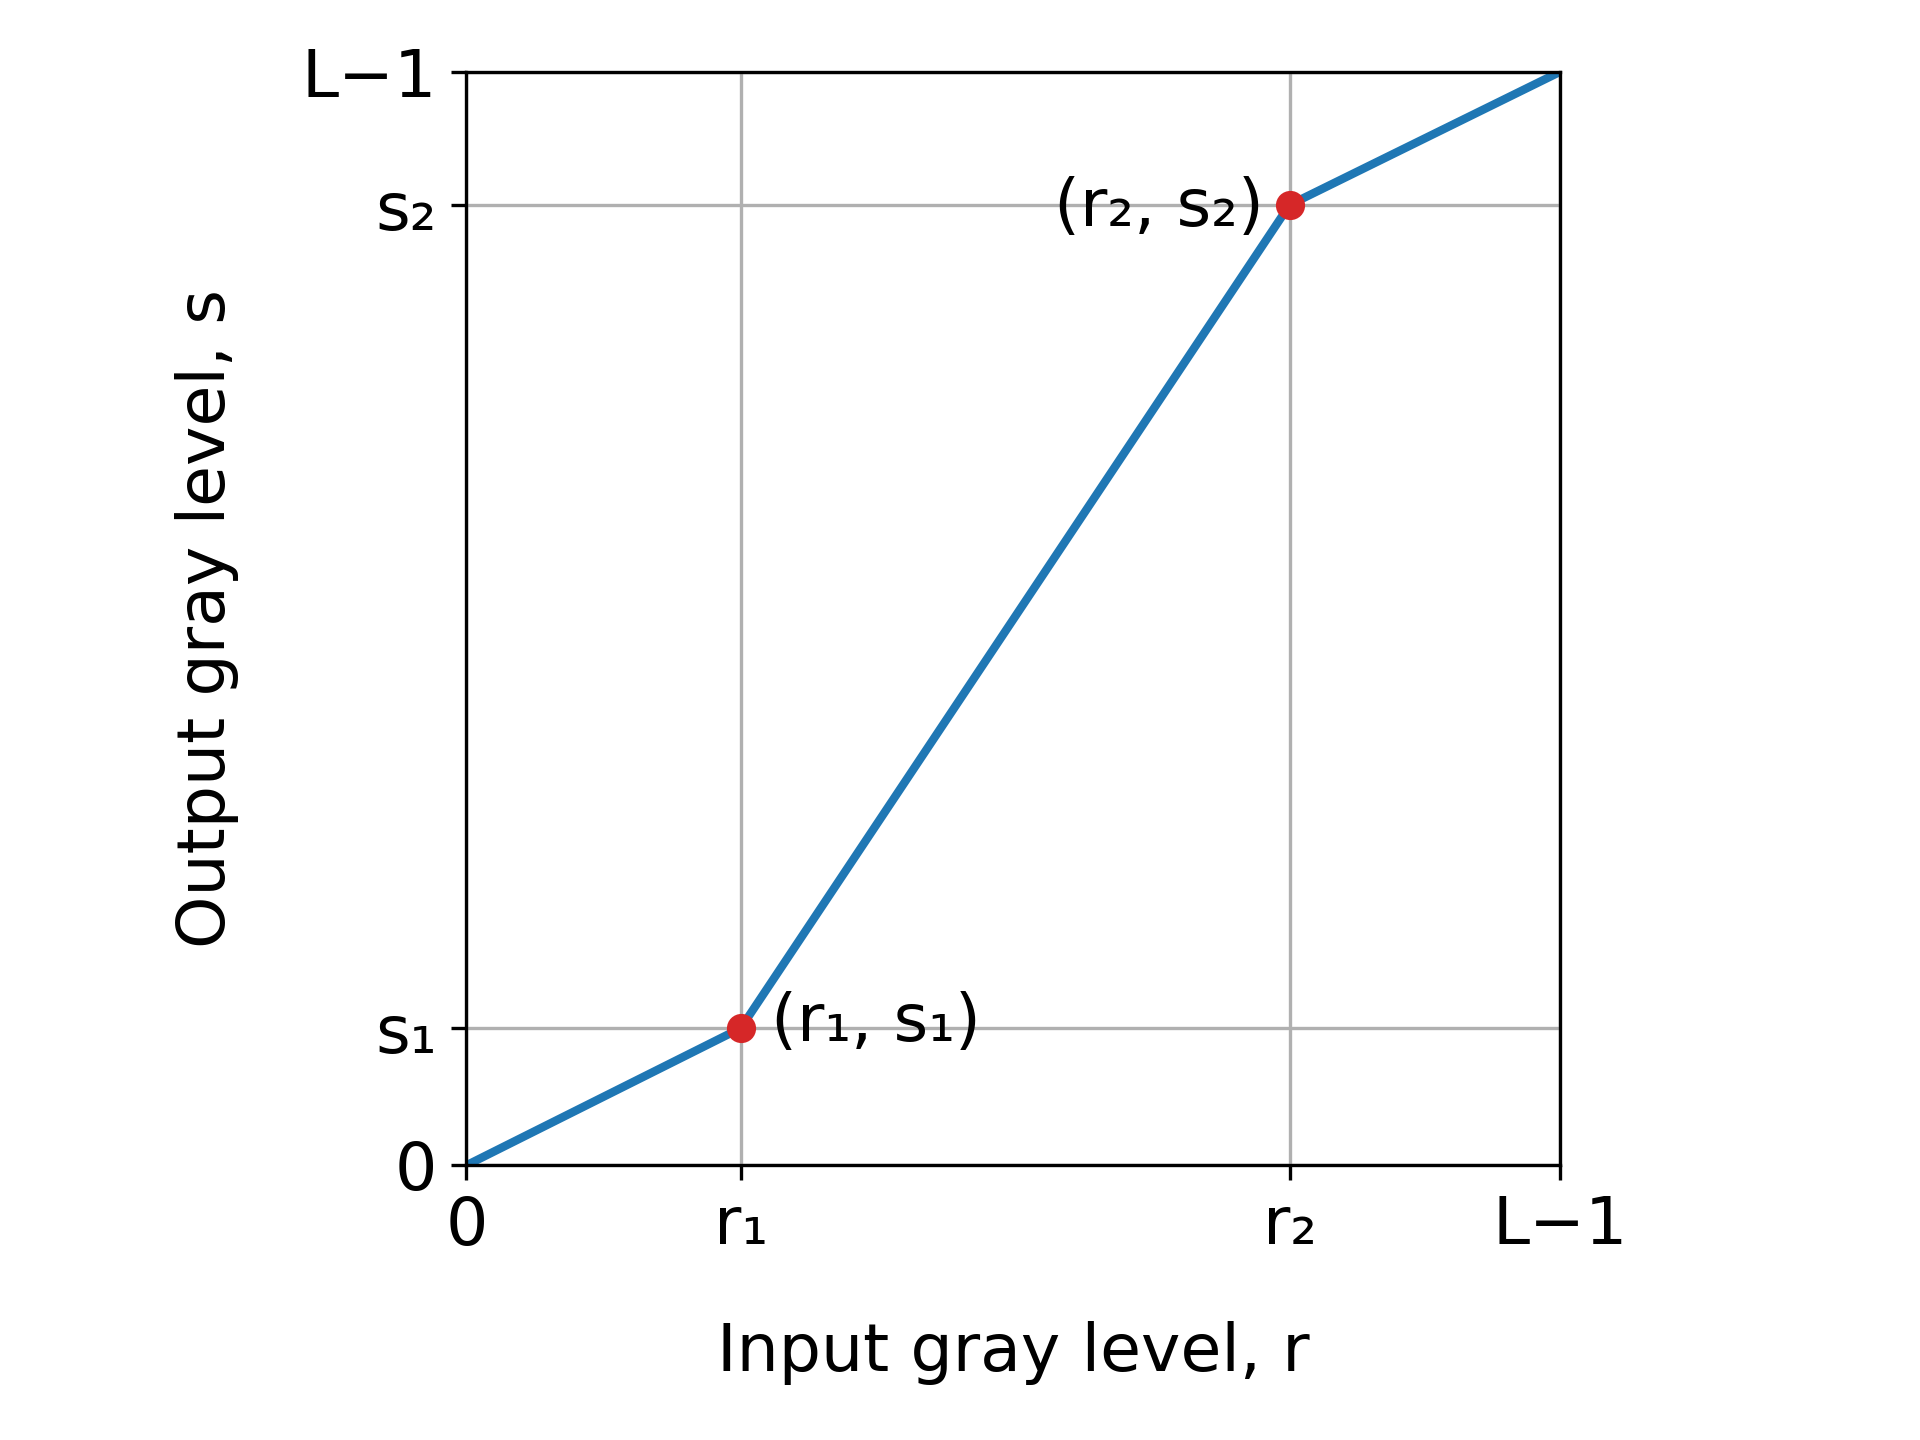
\includegraphics[width=\linewidth]{images/piecewise_transform.png}
        \vspace{-0.5cm}
        \caption{Piecewise linear transform}
      \end{figure}
    \end{minipage}

  \item \textbf{Gray Level Slicing:} Similar to thresholding, but
    allows for a range of pixel values to be highlighted.
    \begin{itemize}
      \item Other levels can be suppressed or maintained
      \item Useful for enhancing specific features in an image
    \end{itemize}

    \begin{minipage}{\linewidth}
      \begin{figure}[H]
        \centering
        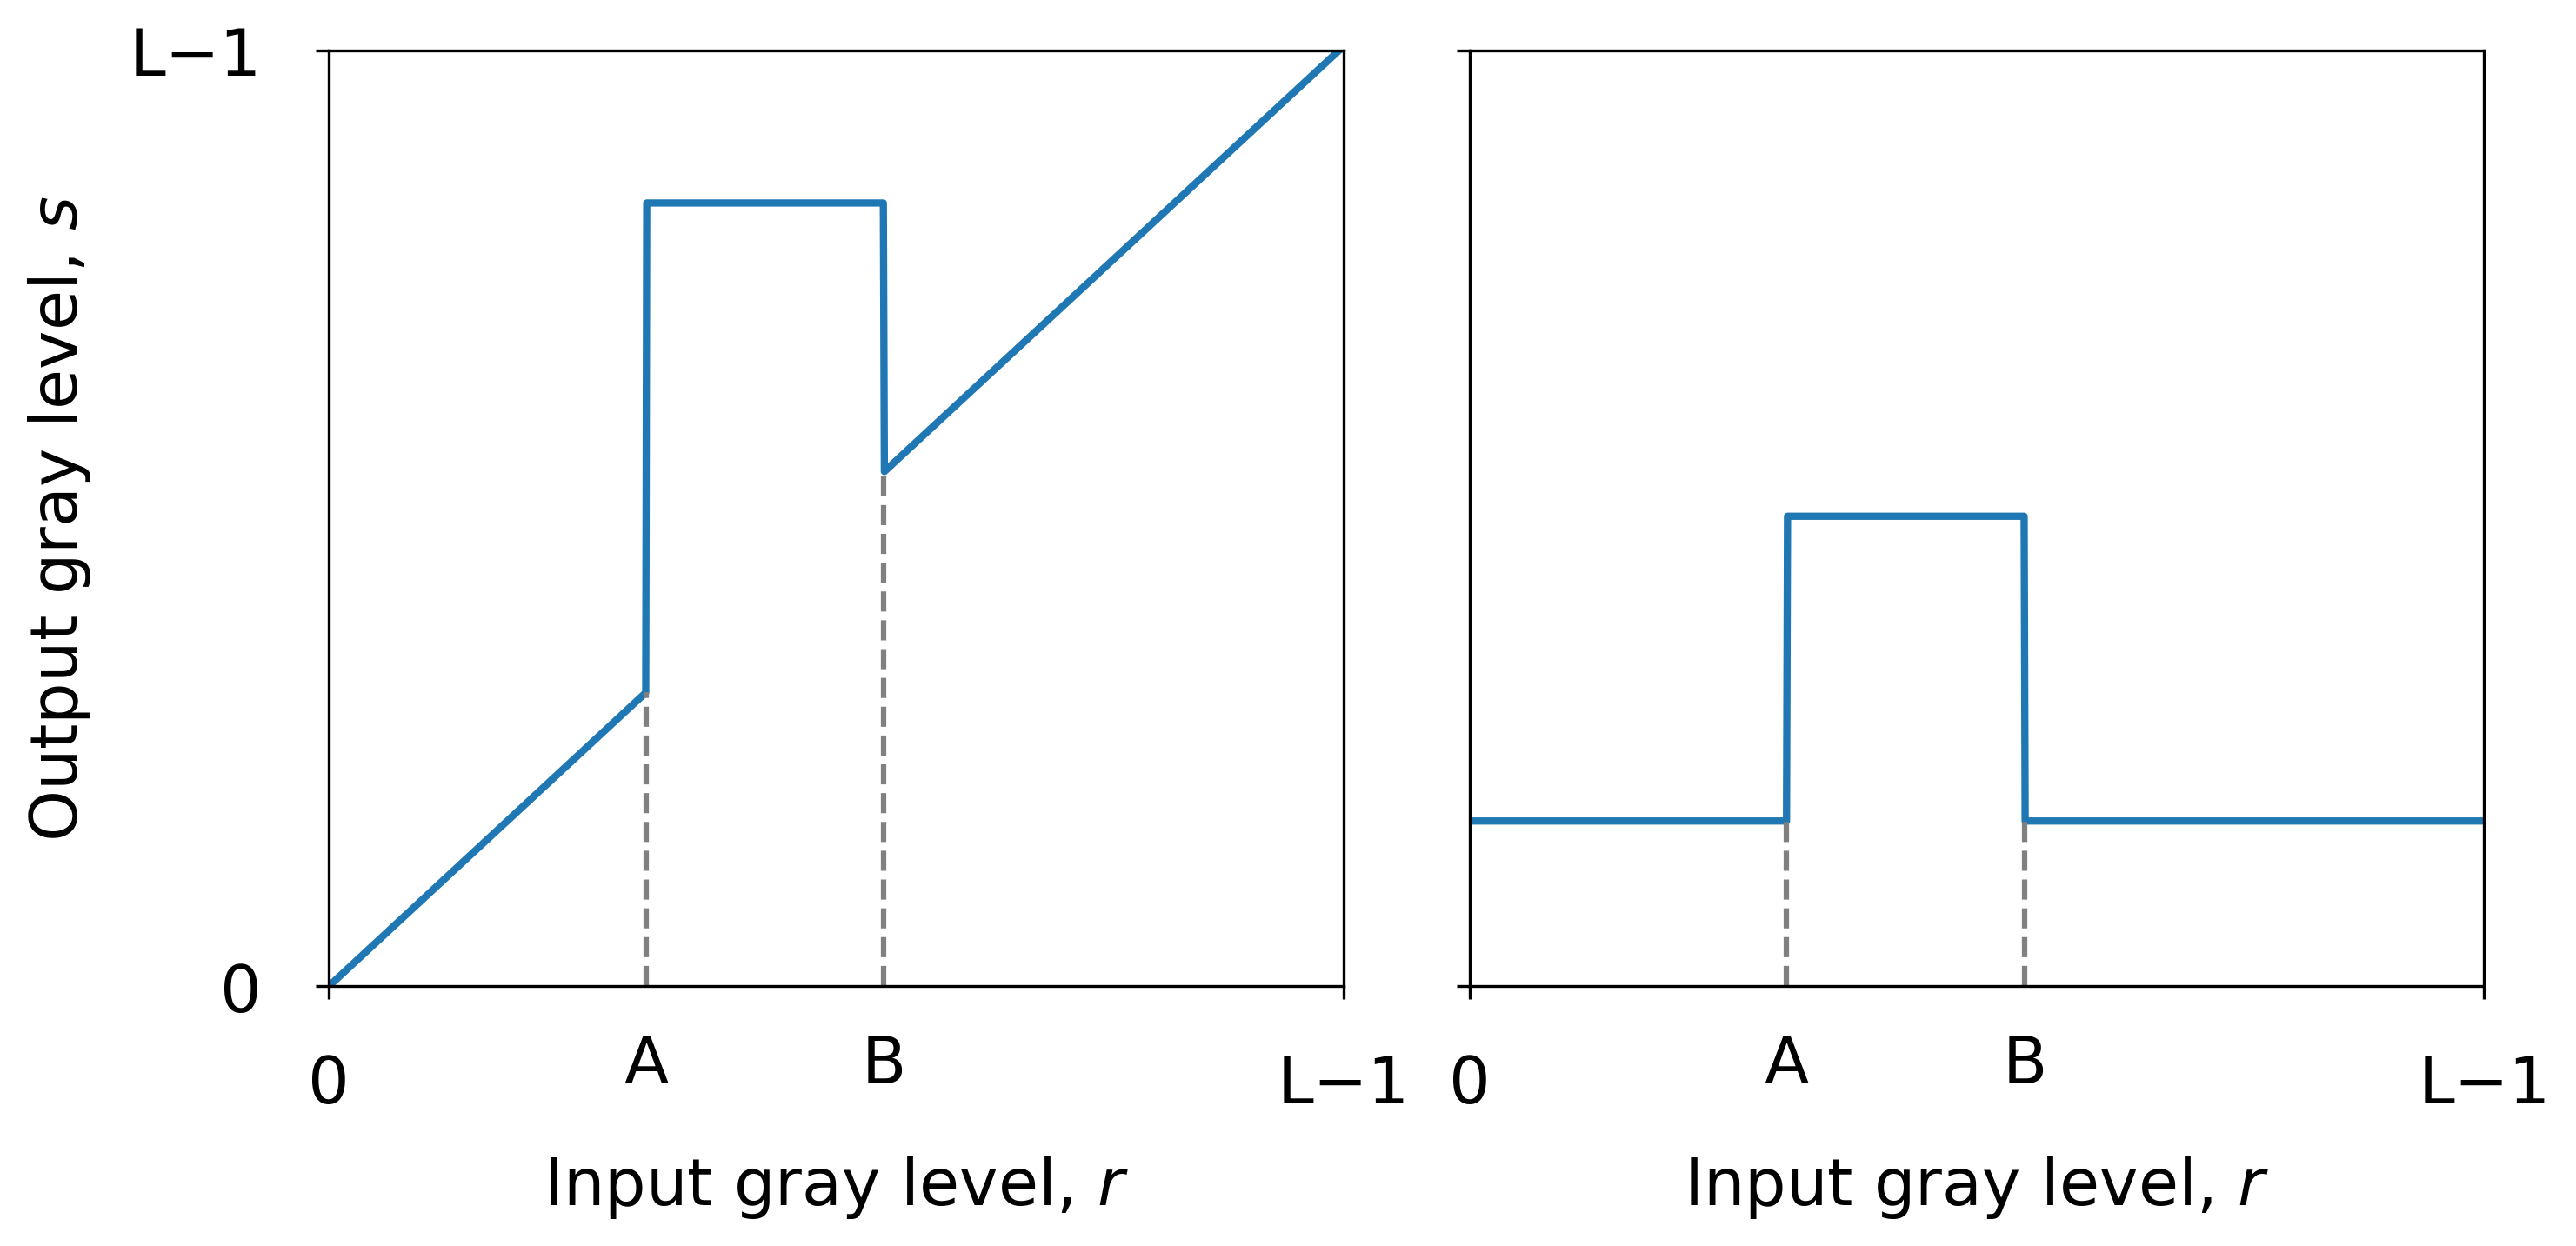
\includegraphics[width=\linewidth]{images/gray_level_slicing.png}
        \caption{Gray level slicing with (i) background retained (ii)
        background supressed}
      \end{figure}
    \end{minipage}

  \item \textbf{Bit-Plane Slicing:} By isolating particular bits of
    the pixel values in an image, we can highligh interesting aspects
    of that image.
    \begin{itemize}
      \item Higher order bits contain most of the significant information
      \item Lower order bits contain subtle details
      \item \enquote{Bit planes} are arranged in a stack; MSB at the
        top, LSB at the bottom.
    \end{itemize}

    \begin{minipage}{\linewidth}
      \begin{figure}[H]
        \centering
        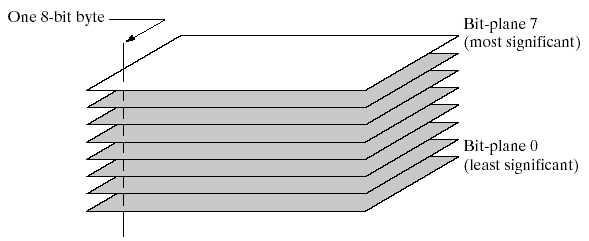
\includegraphics[width=\linewidth]{images/bit_plane_slicing.png}
        \caption{Bit-plane slicing of an 8-bit image}
      \end{figure}
      \vspace{-0.5cm}
    \end{minipage}

\end{itemize}

\subsection*{Neighborhood Operations}

Operations on a \textbf{rectangular region} around a pixel. Any size
rectangle and any shape filter are possible.

\subsubsection*{Simple Neighborhood Operations}

For any pixel $p$ in an image at the center of a neighborhood:

\begin{itemize}
  \item \textbf{Min:} Sets $p$ to minimum value in the neighborhood.
    \begin{itemize}
        \vspace{-0.2cm}
      \item Removes small bright spots (\textbf{salt noise})
      \item Makes \textbf{dark regions darker}
    \end{itemize}
  \item \textbf{Max:} Sets $p$ to maximum value in the neighborhood.
    \begin{itemize}
        \vspace{-0.2cm}
      \item Removes small dark spots (\textbf{pepper noise})
      \item Makes \textbf{bright regions brighter}
    \end{itemize}
  \item \textbf{Median:} Sets $p$ to median value in the neighborhood.
    \begin{itemize}
        \vspace{-0.2cm}
      \item Removes \textbf{salt and pepper noise}
    \end{itemize}
\end{itemize}

\subsubsection*{Spatial Differentiation}

Differentiation measures the \textit{rate of change} of a function.
In the context of image processing, the function is the pixel
intensity, and differentiation helps identify edges and transitions
in the image.

\begin{itemize}
  \item \textbf{First Derivative:} Measures the rate of change of
    pixel intensity.
    \begin{gather*}
      \frac{\partial f}{\partial x} = f(x + 1, y) - f(x, y)\\
      \frac{\partial f}{\partial y} = f(x, y + 1) - f(x, y)
    \end{gather*}
  \item \textbf{Second Derivative:} Measures the rate of change of
    the first derivative.
    \begin{gather*}
      \frac{\partial^2 f}{\partial x^2} = f(x + 1, y) + f(x - 1, y) - 2f(x, y)\\
      \frac{\partial^2 f}{\partial y^2} = f(x, y + 1) + f(x, y - 1) - 2f(x, y)
    \end{gather*}
  \item \textbf{The Laplacian:} Combines the second derivatives in
    both x and y directions.
    \begin{equation*}
      \nabla^2 f = \frac{\partial^2 f}{\partial x^2} +
      \frac{\partial^2 f}{\partial y^2}
    \end{equation*}
    In practice, the Laplacian is applied using a \textbf{filter}.
\end{itemize}

\begin{tblr}{
    colspec={@{}l X[l] | X[l]},
    row{1} = {c, font=\bfseries},
  }
  \cline{2-3}
  & \textbf{First Derivative} & \textbf{Second Derivative} \\
  \cline{2-3}
  \textbullet & Generally produces thicker edges
  & Stronger response to fine detail (e.g.\ thin lines) \\[6pt]
  \textbullet & Stronger response to grey level step
  & Double response to step changes in grey level \\[6pt]
\end{tblr}

\subsubsection*{Correlation vs Convolution}

Most spatial filtering operations are technically
\textbf{correlation}, and the filter is referred to as a
\textbf{correlation kernel} or \textbf{mask}. \textbf{Convolution} is
a similar operation, with a subtle difference:

\begin{figure}[H]
  \centering
  \begin{tikzpicture}[%
      imgcell/.style={draw=black, fill=white, minimum size=1cm, anchor=center},
      filtercell/.style={draw=MaterialBlue900, fill=MaterialBlue50,
      minimum size=1cm, anchor=center}
    ]

    % Original image grid
    \node[imgcell] (i11) at (0,2) {$r_1$};
    \node[imgcell] (i12) at (1,2) {$r_2$};
    \node[imgcell] (i13) at (2,2) {$r_3$};
    \node[imgcell] (i21) at (0,1) {$r_4$};
    \node[imgcell, fill=MaterialGrey200] (i22) at (1,1) {$r_5$};
    \node[imgcell] (i23) at (2,1) {$r_6$};
    \node[imgcell] (i31) at (0,0) {$r_7$};
    \node[imgcell] (i32) at (1,0) {$r_8$};
    \node[imgcell] (i33) at (2,0) {$r_9$};

    % Convolution symbol
    \node at (3,1) {\large $\ast$};

    % Filter grid
    \node[filtercell] (f11) at (4,2) {$k_1$};
    \node[filtercell] (f12) at (5,2) {$k_2$};
    \node[filtercell] (f13) at (6,2) {$k_3$};
    \node[filtercell] (f21) at (4,1) {$k_4$};
    \node[filtercell] (f22) at (5,1) {$k_5$};
    \node[filtercell] (f23) at (6,1) {$k_6$};
    \node[filtercell] (f31) at (4,0) {$k_7$};
    \node[filtercell] (f32) at (5,0) {$k_8$};
    \node[filtercell] (f33) at (6,0) {$k_9$};

  \end{tikzpicture}
  \caption{An image (left) being operated on by a filter (right). The
    result depends
  on whether the operation is correlation or convolution.}
\end{figure}
\vspace{-0.5cm}
\begin{itemize}
  \item \textbf{Correlation:} The filter is applied directly to the
    image, without flipping it.
    \vspace{-0.2cm}
    \begin{equation*}
      s = r_1 k_1 + r_2 k_2 + r_3 k_3 + r_4 k_4 + r_5 k_5 + r_6 k_6 +
      r_7 k_7 + r_8 k_8 + r_9 k_9\\[-0.3cm]
    \end{equation*}
  \item \textbf{Convolution:} The filter is flipped both horizontally
    and vertically before being applied to the image.
    \vspace{-0.2cm}
    \begin{equation*}
      s = r_1 k_9 + r_2 k_8 + r_3 k_7 + r_4 k_6 + r_5 k_5 + r_6 k_4 +
      r_7 k_3 + r_8 k_2 + r_9 k_1\\[-0.3cm]
    \end{equation*}
\end{itemize}

\subsubsection*{Handling Boundary Effects}

Edge pixels don't have a full neighborhood. A filter applied on a
pixel on or near the image boundaries \textbf{may exceed the image
boundaries}, leading to undefined behavior. There are strategies to
handle this:

\begin{minipage}{\linewidth}
  \begin{figure}[H]
    \centering
    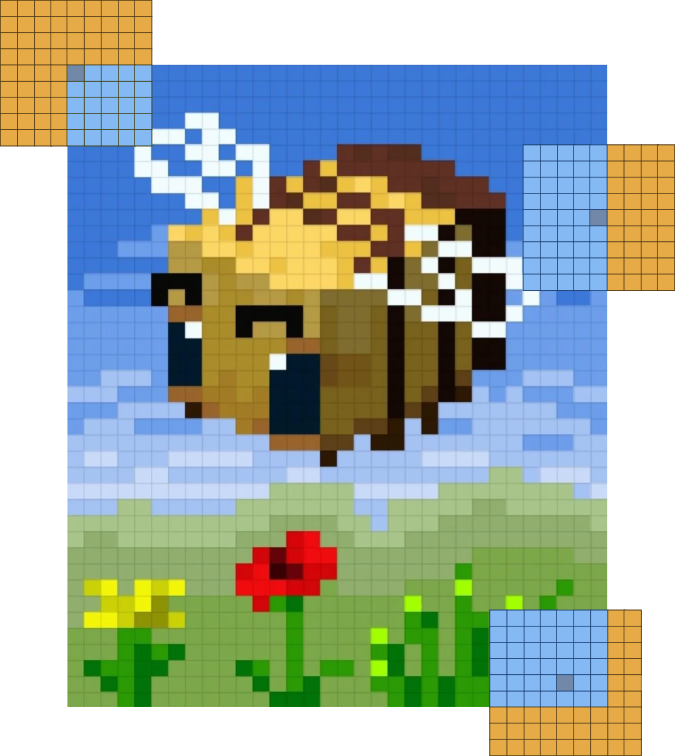
\includegraphics[width=0.6\linewidth]{images/edges.png}
    \caption{A filter may exceed the image boundaries}
  \end{figure}
\end{minipage}

\begin{itemize}
  \item \textbf{Valid (Crop)}: Only compute outputs where the kernel
    lies entirely inside; reduces output size.
  \item \textbf{Partial (Truncate)}: Ignore kernel weights falling
    outside and renormalize the remainder; minor overhead.
  \item \textbf{Constant Pad}: Add a border of fixed-value pixels
    (e.g.\ zero or white) to restore full output dimensions.
  \item \textbf{Replicate}: Extend the nearest edge pixel values
    outward; simple and fast, with minimal artifacts.
  \item \textbf{Reflect}: Mirror the image at its borders; preserves
    continuity but may introduce mirrored features.
\end{itemize}

\subsubsection*{Linear Spatial Filters}

\begin{equation*}
  g(x, y) = \sum_{s=-a}^{a} \sum_{t=-b}^{b} w(s, t) f(x + s, y + t)
\end{equation*}

\begin{itemize}
  \item \textbf{Identity Filter:} Leaves the image unchanged. Simply
    assigns a weight \enquote{0} to all the neighbors around the central pixel.

    \begin{minipage}{\linewidth}
      \vspace{-0.3cm}
      \begin{figure}[H]
        \centering
        \begin{tikzpicture}[%
            filtercell/.style={draw=MaterialBlue900, fill=MaterialBlue50,
            minimum size=1cm, anchor=center}
          ]
          \node[filtercell] (f11) at (0,2) {$0$};
          \node[filtercell] (f12) at (1,2) {$0$};
          \node[filtercell] (f13) at (2,2) {$0$};
          \node[filtercell] (f21) at (0,1) {$0$};
          \node[filtercell] (f22) at (1,1) {$1$};
          \node[filtercell] (f23) at (2,1) {$0$};
          \node[filtercell] (f31) at (0,0) {$0$};
          \node[filtercell] (f32) at (1,0) {$0$};
          \node[filtercell] (f33) at (2,0) {$0$};

        \end{tikzpicture}
        \caption{Identity filter}
      \end{figure}
    \end{minipage}
  \item \textbf{Smoothing Filters:} Smooths an image by averaging
    pixel values in the neighborhood.
    \begin{itemize}
      \item \textbf{Mean filter} or \textbf{simple
        averaging filter}: simplest form; $k \times k$ matrix, each
        element is $1/k^2$.

        \begin{minipage}{\linewidth}
          \vspace{-0.3cm}
          \begin{figure}[H]
            \centering
            \begin{tikzpicture}[%
                filtercell/.style={draw=MaterialBlue900, fill=MaterialBlue50,
                minimum size=1cm, anchor=center}
              ]
              \node[filtercell] (f11) at (0,2) {$1/9$};
              \node[filtercell] (f12) at (1,2) {$1/9$};
              \node[filtercell] (f13) at (2,2) {$1/9$};
              \node[filtercell] (f21) at (0,1) {$1/9$};
              \node[filtercell] (f22) at (1,1) {$1/9$};
              \node[filtercell] (f23) at (2,1) {$1/9$};
              \node[filtercell] (f31) at (0,0) {$1/9$};
              \node[filtercell] (f32) at (1,0) {$1/9$};
              \node[filtercell] (f33) at (2,0) {$1/9$};

            \end{tikzpicture}
            \caption{Simple 3x3 averaging filter}
          \end{figure}
        \end{minipage}
      \item \textbf{Weighted averaging filter}: Sometimes different
        pixels in the neighborhood are weighted differently; the
        filter values always add up to 1.

        \begin{minipage}{\linewidth}
          \vspace{-0.3cm}
          \begin{figure}[H]
            \centering
            \begin{tikzpicture}[%
                filtercell/.style={draw=MaterialBlue900, fill=MaterialBlue50,
                minimum size=1cm, anchor=center}
              ]
              \node[filtercell] (f11) at (0,2) {$1/16$};
              \node[filtercell] (f12) at (1,2) {$2/16$};
              \node[filtercell] (f13) at (2,2) {$1/16$};
              \node[filtercell] (f21) at (0,1) {$2/16$};
              \node[filtercell] (f22) at (1,1) {$4/16$};
              \node[filtercell] (f23) at (2,1) {$2/16$};
              \node[filtercell] (f31) at (0,0) {$1/16$};
              \node[filtercell] (f32) at (1,0) {$2/16$};
              \node[filtercell] (f33) at (2,0) {$1/16$};

            \end{tikzpicture}
            \caption{Weighted 3x3 averaging filter}
          \end{figure}
        \end{minipage}

      \item \textbf{Useful for}: (i) removing noise from images (ii)
        highlighting gross details
    \end{itemize}
  \item \textbf{Sharpening Filters:} Enhances edges, removes blurring
    and fine details in an image.
    \begin{itemize}
      \item \textbf{Laplacian Filter:} Highlights regions of rapid
        intensity change (edges and other discontinuities).
        \begin{itemize}
          \item The Laplacian output is \textbf{not an enhanced
            image}; it is an image with those regions highlighted,
            where the pixel values change rapidly in the original
            image (edges etc.)
          \item In order to obtain the enhanced image, the Laplacian
            output is \textbf{subtracted} from the original image.
          \item This above operation can be summarized as a new
            filter: identity minus Laplacian.
        \end{itemize}

        \begin{minipage}{\linewidth}
          \vspace{-0.3cm}
          \begin{figure}[H]
            \centering
            \begin{tikzpicture}[%
                filtercell/.style={draw=MaterialBlue900, fill=MaterialBlue50,
                minimum size=1cm, anchor=center}
              ]
              \node[filtercell] (f111) at (0,2) {$0$};
              \node[filtercell] (f112) at (1,2) {$1$};
              \node[filtercell] (f113) at (2,2) {$0$};
              \node[filtercell] (f121) at (0,1) {$1$};
              \node[filtercell] (f122) at (1,1) {$4$};
              \node[filtercell] (f123) at (2,1) {$1$};
              \node[filtercell] (f131) at (0,0) {$0$};
              \node[filtercell] (f132) at (1,0) {$1$};
              \node[filtercell] (f133) at (2,0) {$0$};

              \node[filtercell] (f211) at (4,2) {$0$};
              \node[filtercell] (f212) at (5,2) {$-1$};
              \node[filtercell] (f213) at (6,2) {$0$};
              \node[filtercell] (f221) at (4,1) {$-1$};
              \node[filtercell] (f222) at (5,1) {$5$};
              \node[filtercell] (f223) at (6,1) {$-1$};
              \node[filtercell] (f231) at (4,0) {$0$};
              \node[filtercell] (f232) at (5,0) {$-1$};
              \node[filtercell] (f233) at (6,0) {$0$};
            \end{tikzpicture}
            \caption{Laplacian filter (left), Identity minus
            Laplacian filter (right)}
          \end{figure}
        \end{minipage}

      \item \textbf{Unsharp Mask and High-Boost Filtering:} These are
        filters that enhance edges by subtracting a blurred version
        of the image ($\bar{f}(x, y)$) from the original image ($f(x, y)$)
        \begin{gather*}
          f_\textnormal{s}(x, y) = f(x, y) - \bar{f}(x, y)\\
          f_\textnormal{hb}(x, y) = Af(x, y) - \bar{f}(x, y)
        \end{gather*}
        \begin{itemize}
          \item High-boost filtering ($f_\textnormal{hb}$) takes a
            strength parameter $A$. Unsharp mask ($f_\textnormal{s}$)
            is a special case of high-boost filtering with $A = 1$.
        \end{itemize}
    \end{itemize}
    \begin{minipage}{\linewidth}
      \vspace{-0.3cm}
      \begin{figure}[H]
        \centering
        \begin{tikzpicture}[%
            filtercell/.style={draw=MaterialBlue900, fill=MaterialBlue50,
            minimum size=1cm, anchor=center}
          ]
          \node[filtercell] (f111) at (0,2) {$0$};
          \node[filtercell] (f112) at (1,2) {$-1$};
          \node[filtercell] (f113) at (2,2) {$0$};
          \node[filtercell] (f121) at (0,1) {$-1$};
          \node[filtercell] (f122) at (1,1) {\small \hspace{-0.5em} $A + 4$};
          \node[filtercell] (f123) at (2,1) {$-1$};
          \node[filtercell] (f131) at (0,0) {$0$};
          \node[filtercell] (f132) at (1,0) {$-1$};
          \node[filtercell] (f133) at (2,0) {$0$};

          \node[filtercell] (f211) at (4,2) {$-1$};
          \node[filtercell] (f212) at (5,2) {$-1$};
          \node[filtercell] (f213) at (6,2) {$-1$};
          \node[filtercell] (f221) at (4,1) {$-1$};
          \node[filtercell] (f222) at (5,1) {\small \hspace{-0.5em} $A + 8$};
          \node[filtercell] (f223) at (6,1) {$-1$};
          \node[filtercell] (f231) at (4,0) {$-1$};
          \node[filtercell] (f232) at (5,0) {$-1$};
          \node[filtercell] (f233) at (6,0) {$-1$};
        \end{tikzpicture}
        \caption{Two forms of unsharp mask}
      \end{figure}
    \end{minipage}

    For the specific case of a 3x3 filter, the unsharp mask perfectly
    matches the \enquote{identity minus Laplacian filter}!

  \item \textbf{Sobel Filters:} Based on 1st derivative filtering,
    these are typically used for edge detection.
    \begin{itemize}
      \item The Sobel filters are based on the calculation of
        gradients in the x and y directions. As such, there are two
        filters, one for $G_x$ and one for $G_y$.
      \item To filter an image, (i) both the filters are applied and
        (ii) the results are added together.
    \end{itemize}

    \begin{minipage}{\linewidth}
      \vspace{-0.3cm}
      \begin{figure}[H]
        \centering
        \begin{tikzpicture}[%
            filtercell/.style={draw=MaterialBlue900, fill=MaterialBlue50,
            minimum size=1cm, anchor=center}
          ]
          \node[filtercell] (f111) at (0,2) {$-1$};
          \node[filtercell] (f112) at (1,2) {$0$};
          \node[filtercell] (f113) at (2,2) {$1$};
          \node[filtercell] (f121) at (0,1) {$-2$};
          \node[filtercell] (f122) at (1,1) {$0$};
          \node[filtercell] (f123) at (2,1) {$2$};
          \node[filtercell] (f131) at (0,0) {$-1$};
          \node[filtercell] (f132) at (1,0) {$0$};
          \node[filtercell] (f133) at (2,0) {$1$};

          \node[filtercell] (f211) at (4,2) {$-1$};
          \node[filtercell] (f212) at (5,2) {$-2$};
          \node[filtercell] (f213) at (6,2) {$-1$};
          \node[filtercell] (f221) at (4,1) {$0$};
          \node[filtercell] (f222) at (5,1) {$0$};
          \node[filtercell] (f223) at (6,1) {$0$};
          \node[filtercell] (f231) at (4,0) {$1$};
          \node[filtercell] (f232) at (5,0) {$2$};
          \node[filtercell] (f233) at (6,0) {$1$};
        \end{tikzpicture}
        \caption{The Sobel filters for $G_x$/horizontal derivative
        (left) and $G_y$/vertical derivative (right)}
      \end{figure}
    \end{minipage}
\end{itemize}

\section*{Frequency Domain Enhancement}

\subsection*{Fourier Transform}

\textbf{Idea:} Any function that periodically repeats itself
can be expressed as a sum of sines and cosines of different
frequencies each multiplied by a different coefficient

\begin{figure}[H]
  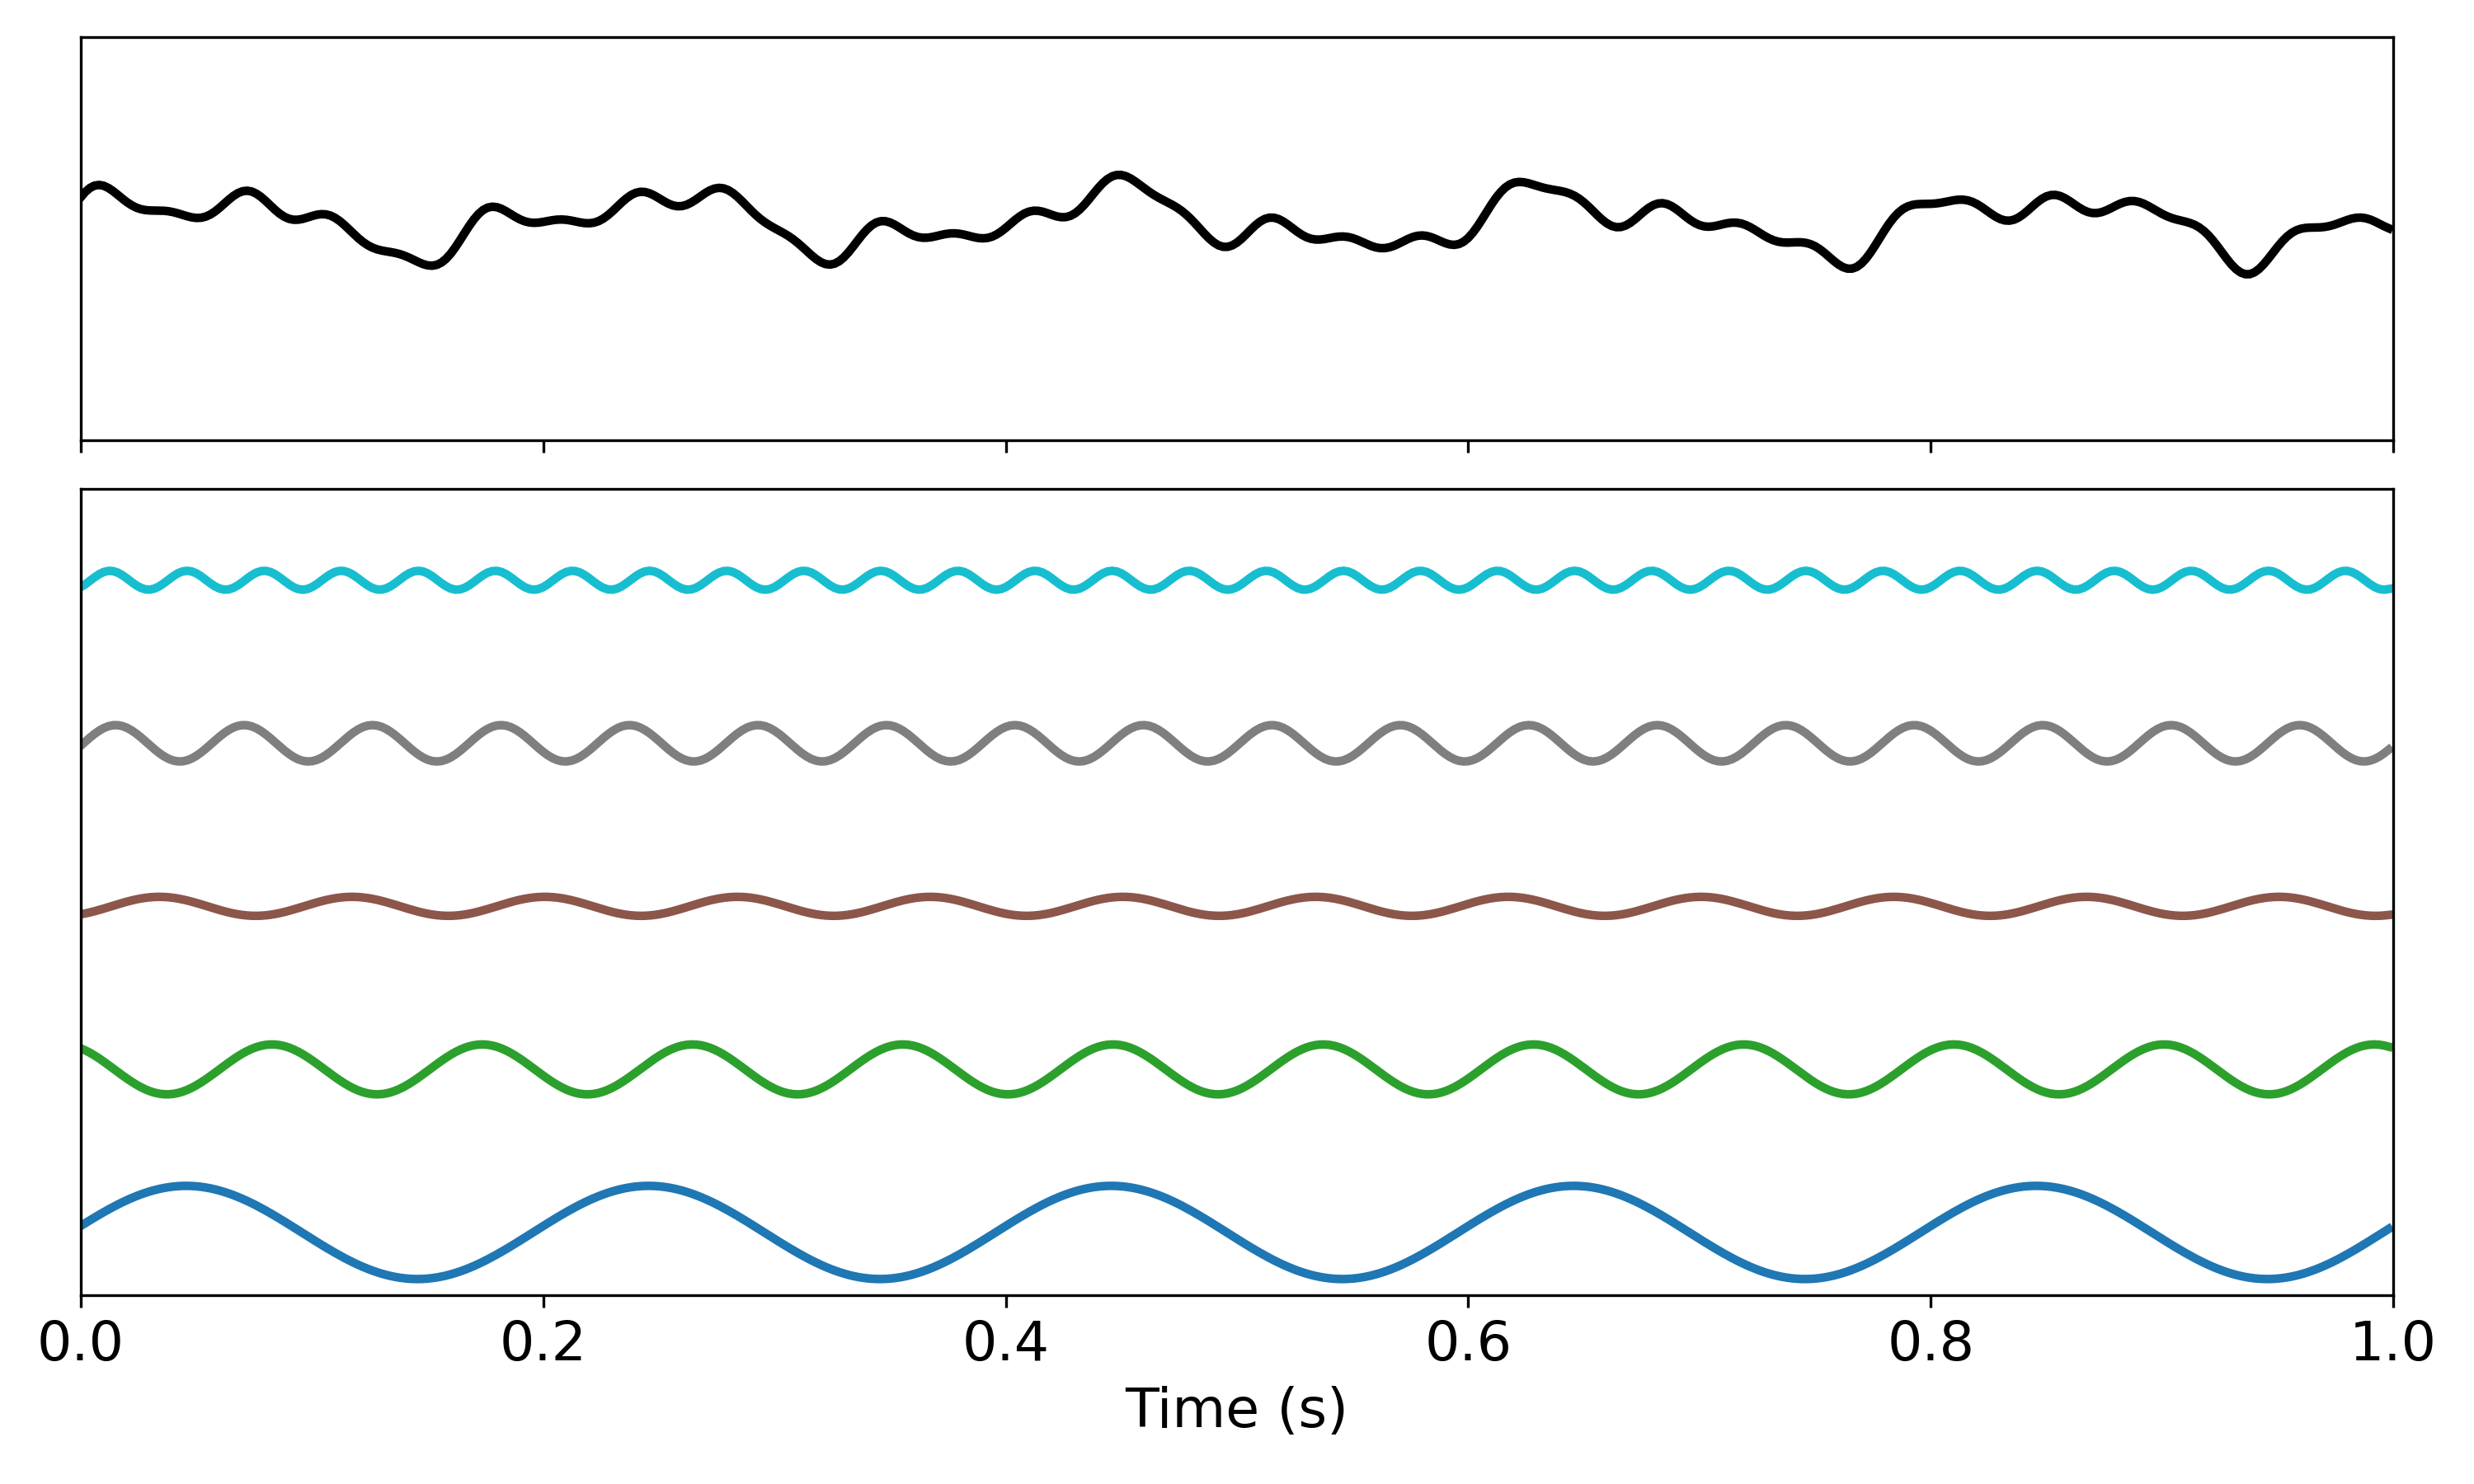
\includegraphics[width=\linewidth]{images/fourier.png}
  \caption{A wave (top) and its Fourier components (bottom)}
\end{figure}

\subsubsection*{Discrete Fourier Transform (DFT)}

\textit{Discrete Fourier Transform} of $f(x, y)$ for $x = 0 \ldots
M-1$ and $y = 0 \ldots N-1$ is defined as:
\begin{equation*}
  F(u, v) = \sum_{x=0}^{M-1} \sum_{y=0}^{N-1} f(x, y)
  e^{-j2\pi\left(ux/M + vy/N\right)}
\end{equation*}

\subsubsection*{DFT and Images}

The DFT of a two dimensional image can be visualized by showing the
spectrum of the image's component frequencies.

\begin{figure}[H]
  \centering
  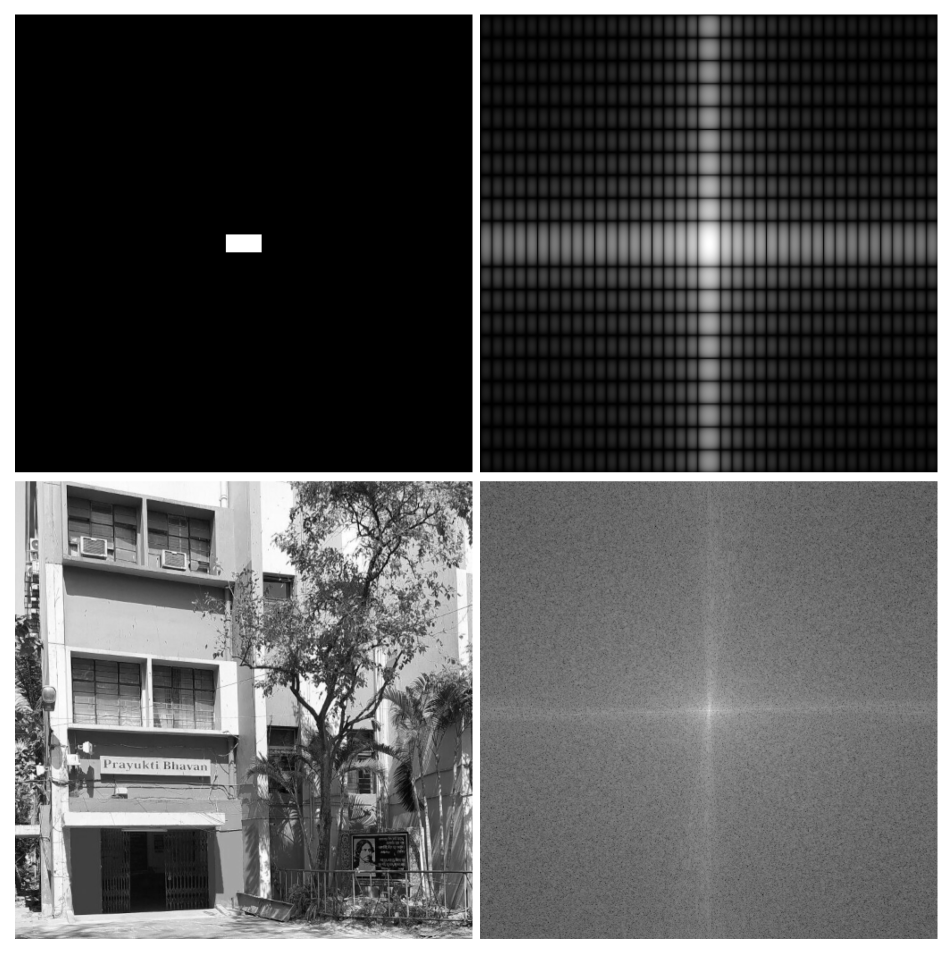
\includegraphics[width=\linewidth]{images/dft_spectra.png}
  \caption{(i) Image of a simple black rectangle and its spectrum
  (top) (ii) Photograph of a building and its spectrum (bottom)}
\end{figure}

\subsubsection*{Inverse DFT}

The Fourier transform is \textbf{completely invertible}. The inverse
DFT of $F(u, v)$ for $u = 0 \ldots M-1$ and $v = 0 \ldots N-1$ is defined as:

\begin{equation*}
  f(x, y) = \frac{1}{MN} \sum_{u=0}^{M-1} \sum_{v=0}^{N-1} F(u, v)
  e^{j2\pi\left(ux/M + vy/N\right)}
\end{equation*}

\subsubsection*{Frequency Domain Filtering}

\begin{figure}[H]
  \centering
  \begin{tikzpicture}[
      node distance=0.8cm and 0.6cm,
      every node/.style={
        align=center
      },
      >={Stealth}
    ]
    % Row 1
    \node (n1) {Input Image\\$f(x,y)$};
    \node (n2) [draw, right=of n1] {Preprocessing};
    \node (n3) [draw, right=of n2] {Fourier Transform};

    % Row 2
    \node (n4) [draw, below=of n3] {Filter Function\\$H(u, v)$};
    \node (n5) [draw, left=4cm of n4] {Inverse Fourier\\Transform};
    \node (n6) [draw, below=of n5] {Post Processing};

    % Row 3
    \node (n7) [right=of n6] {Enhanced Image\\$g(x,y)$};

    % Sequential arrows
    \draw[->] (n1) -- (n2);
    \draw[->] (n2) -- (n3);
    \draw[->] (n3) -- node [right] {$F(u, v)$} (n4);
    \draw[->] (n4) -- node [above] {$F(u, v) * H(u, v)$} (n5);
    \draw[->] (n5) -- (n6);
    \draw[->] (n6) -- (n7);
  \end{tikzpicture}
\end{figure}

Let us define $D(u, v) = \sqrt{(u - \frac{M}{2})^2 + (v -
\frac{N}{2})^2}$, the distance of the point $(u, v)$ from the origin
of the transform. Frequency domain filters are functions of $D(u, v)$.

\begin{itemize}
  \item \textbf{Smoothing filters:} In frequency domain, smoothing is
    achieved by dropping out the high frequency components.
    \begin{itemize}
      \item \textbf{Ideal low-pass filter:} Simply cut off all high
        frequency components that are a specified distance $D_0$ from the
        origin of the transform. Changing $D_0$ changes the behavior
        of the filter.

        \begin{minipage}{\linewidth}
          \begin{figure}[H]
            \centering
            \includegraphics[width=\linewidth]{images/ideal_low_pass.png}
          \end{figure}
        \end{minipage}

        \begin{equation*}
          H(u, v) =
          \begin{cases}
            1 & \text{if } D(u, v) \leq D_0 \\
            0 & \text{otherwise}
          \end{cases}
        \end{equation*}

      \item \textbf{Butterworth Low-pass filter:} A smoother
        transition between the pass and stop bands than the ideal low-pass
        filter. With order $n$ and cutoff frequency $D_0$:

        \begin{minipage}{\linewidth}
          \begin{figure}[H]
            \centering
            \includegraphics[width=\linewidth]{images/butterworth_low_pass.png}
          \end{figure}
        \end{minipage}

        \begin{equation*}
          H(u, v) = \frac{1}{1 + (D(u, v)/D_0)^{2n}}
        \end{equation*}

      \item \textbf{Gaussian Low-pass filter:} A Gaussian function
        that smoothly decays to zero as $D(u, v)$ increases. With cutoff
        frequency $D_0$:

        \begin{minipage}{\linewidth}
          \begin{figure}[H]
            \centering
            \includegraphics[width=\linewidth]{images/gaussian_low_pass.png}
          \end{figure}
        \end{minipage}

        \begin{equation*}
          H(u, v) = e^{-D(u, v)^2/2D_0^2}
        \end{equation*}

        \begin{itemize}
          \item Gaussian filters are often used to correct \textbf{broken
            characters} in low resolution text images.

            \begin{minipage}{\linewidth}
              \vspace{-0.5cm}
              \begin{figure}[H]
                \centering
                \includegraphics[width=\linewidth]{images/gaussian_text_correction.png}
                \caption{Gaussian filter can correct broken characters}
              \end{figure}
            \end{minipage}

          \item Gaussian filters can also \textbf{remove blemishes in
            photographs}

            \begin{minipage}{\linewidth}
              \vspace{-0.4cm}
              \begin{figure}[H]
                \centering
                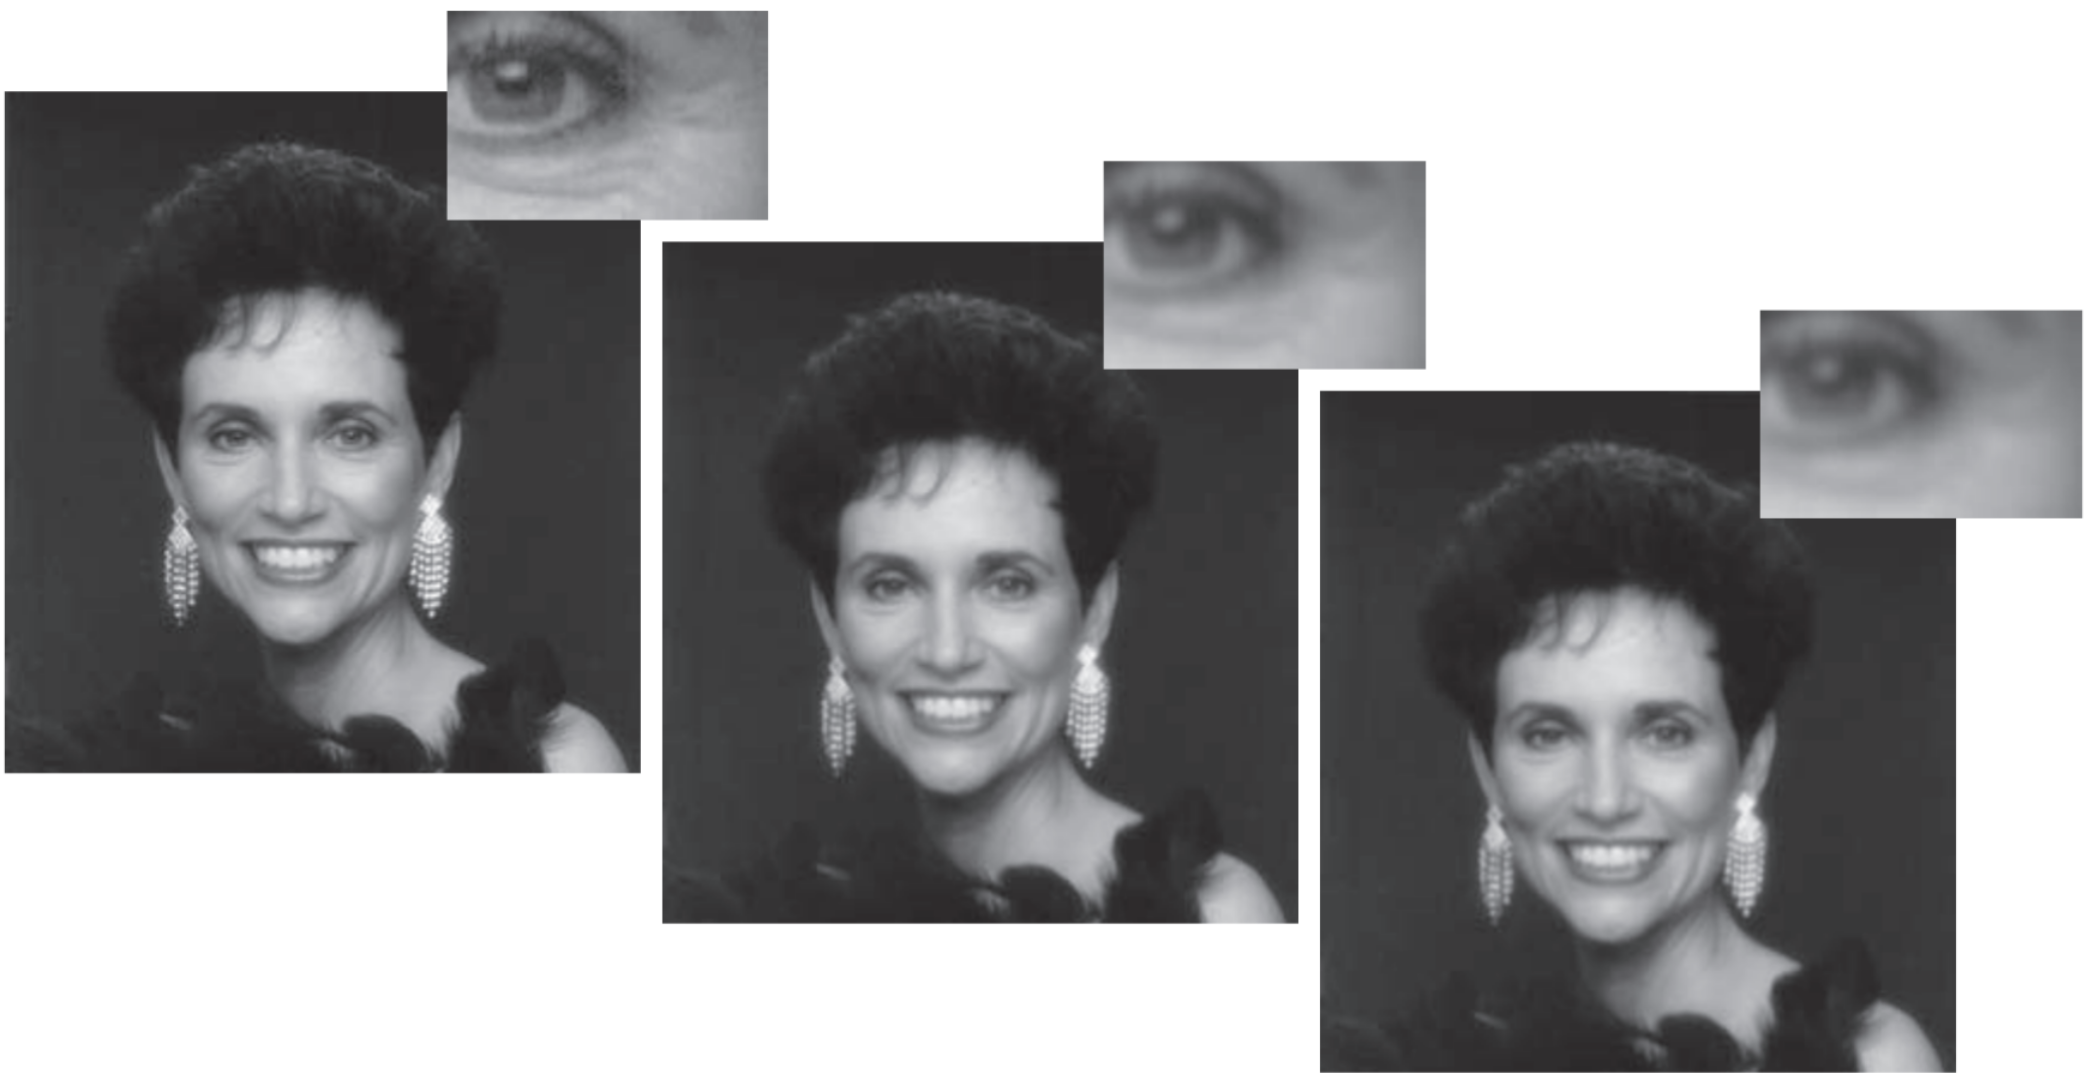
\includegraphics[width=\linewidth]{images/gaussian_photo_correction.png}
                \caption{Gaussian filter can remove blemishes in photographs}
              \end{figure}
            \end{minipage}
        \end{itemize}
    \end{itemize}

  \item \textbf{Sharpening filters:} Edges and fine details are
    associated with high frequency components.

    \begin{itemize}
      \item \textbf{Ideal high-pass filter:} Cut off all low
        frequency components that are a specified distance $D_0$ from
        the origin of the transform.

        \begin{minipage}{\linewidth}
          \begin{figure}[H]
            \centering
            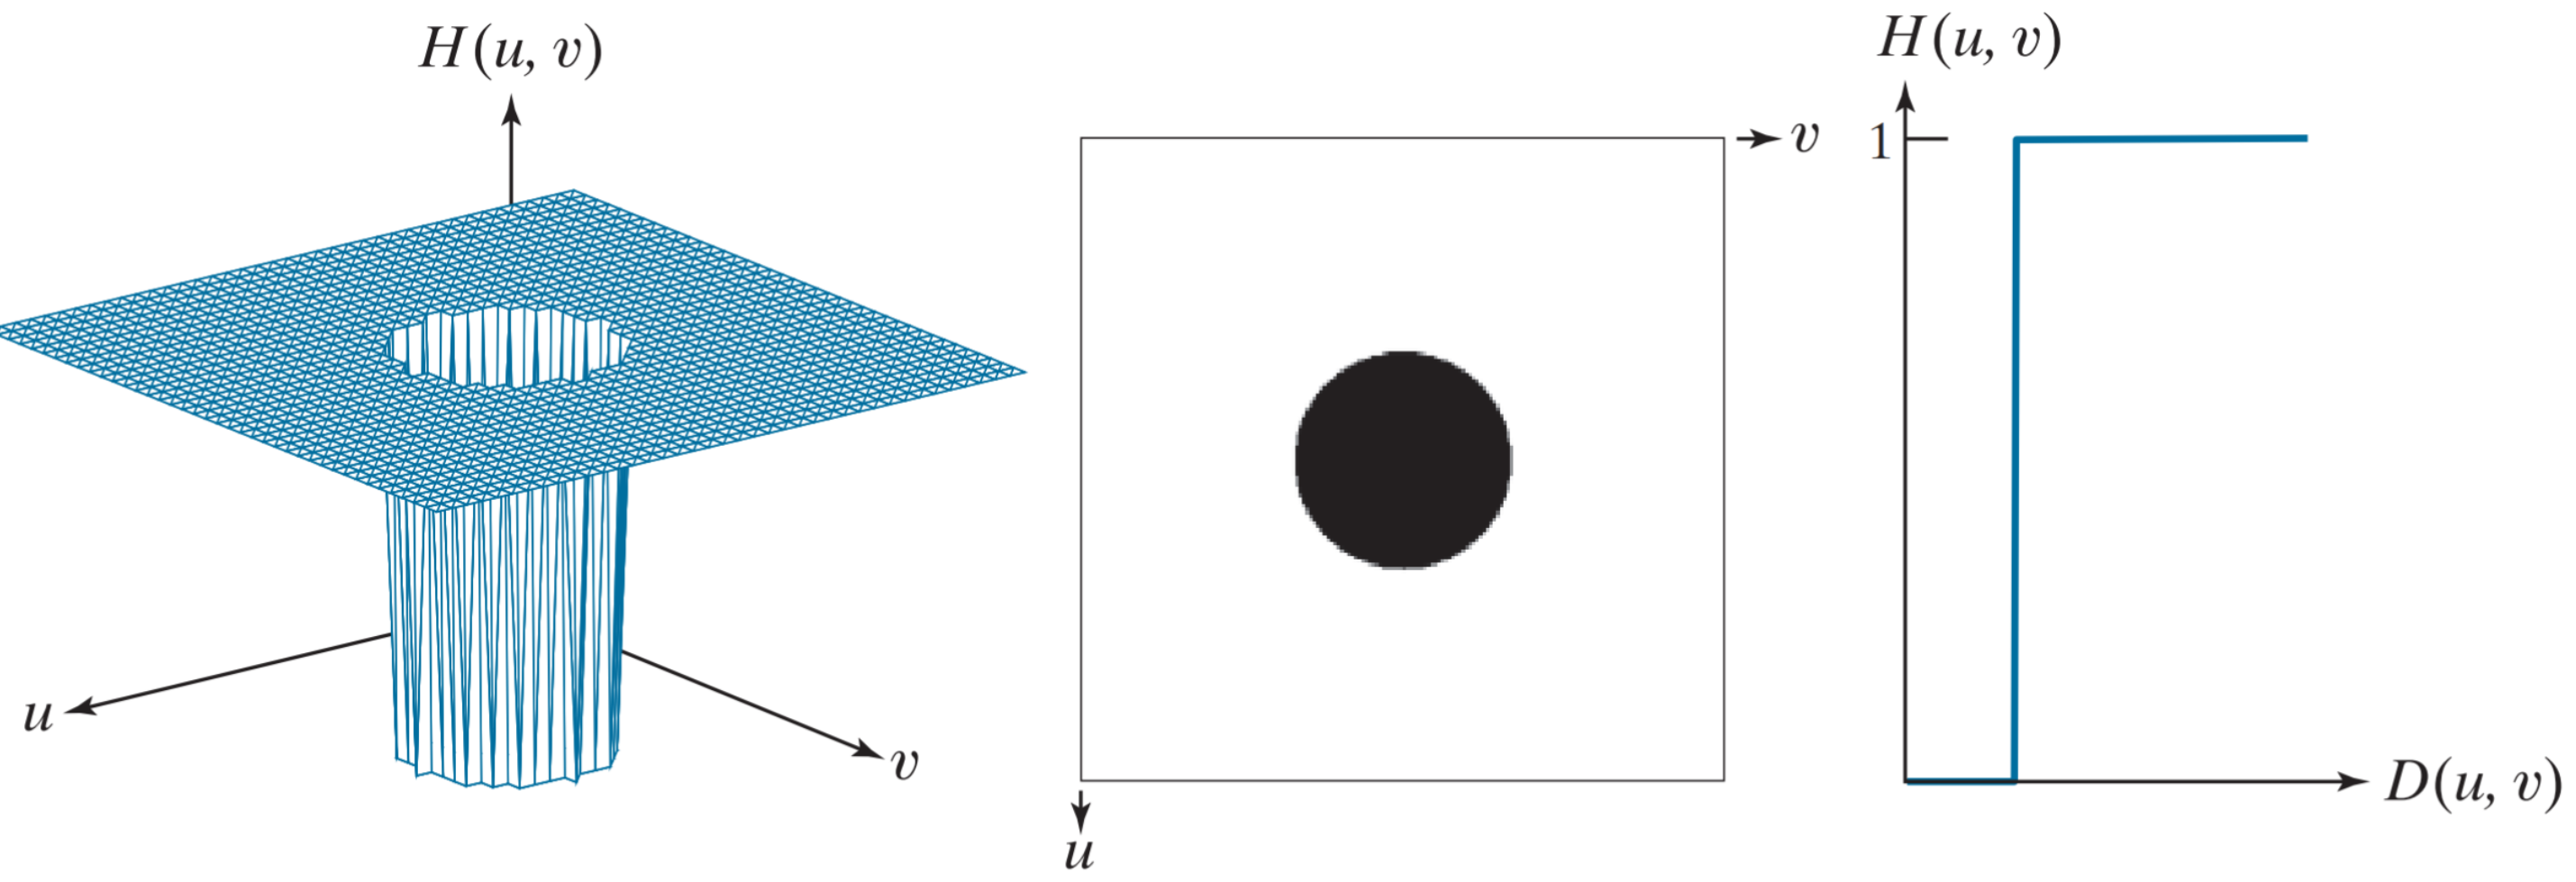
\includegraphics[width=\linewidth]{images/ideal_high_pass.png}
          \end{figure}
        \end{minipage}

        \begin{equation*}
          H_\text{hp}(u, v) = 1 - H_\text{lp}(u, v) =
          \begin{cases}
            0 & \text{if } D(u, v) \leq D_0 \\
            1 & \text{otherwise}
          \end{cases}
        \end{equation*}

      \item \textbf{Butterworth High-pass filter:} A smoother
        transition between the pass and stop bands than the ideal high-pass
        filter. With order $n$ and cutoff frequency $D_0$:

        \begin{minipage}{\linewidth}
          \begin{figure}[H]
            \centering
            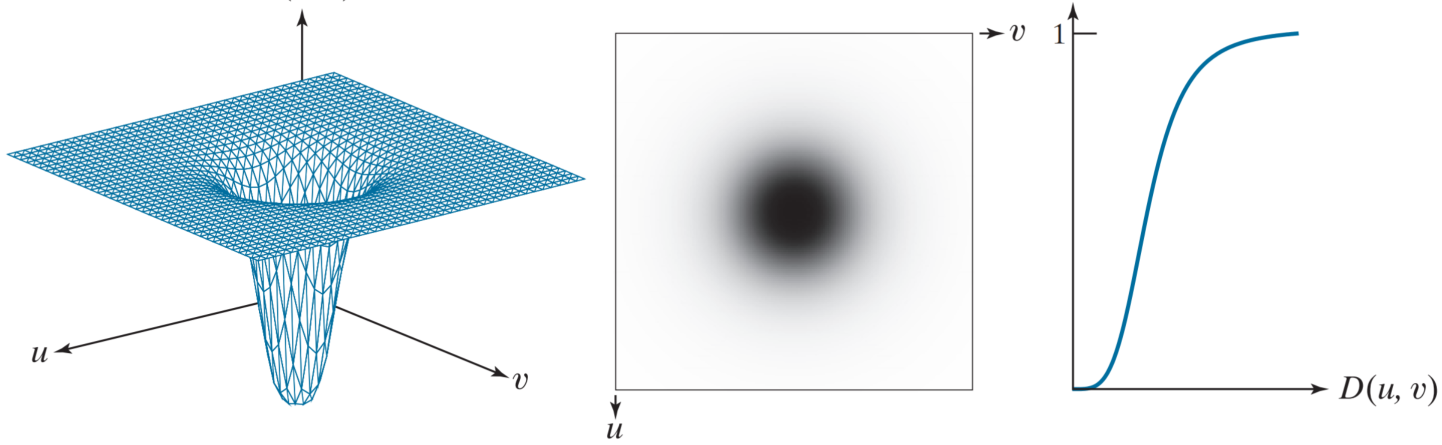
\includegraphics[width=\linewidth]{images/butterworth_high_pass.png}
          \end{figure}
        \end{minipage}

        \begin{equation*}
          H_\text{hp}(u, v) = \frac{1}{1 + (D_0/D_(u, v))^{2n}}
        \end{equation*}

      \item \textbf{Gaussian High-pass filter:} A Gaussian function
        that smoothly increases to 1 as $D(u, v)$ increases. With cutoff
        frequency $D_0$:

        \begin{minipage}{\linewidth}
          \begin{figure}[H]
            \centering
            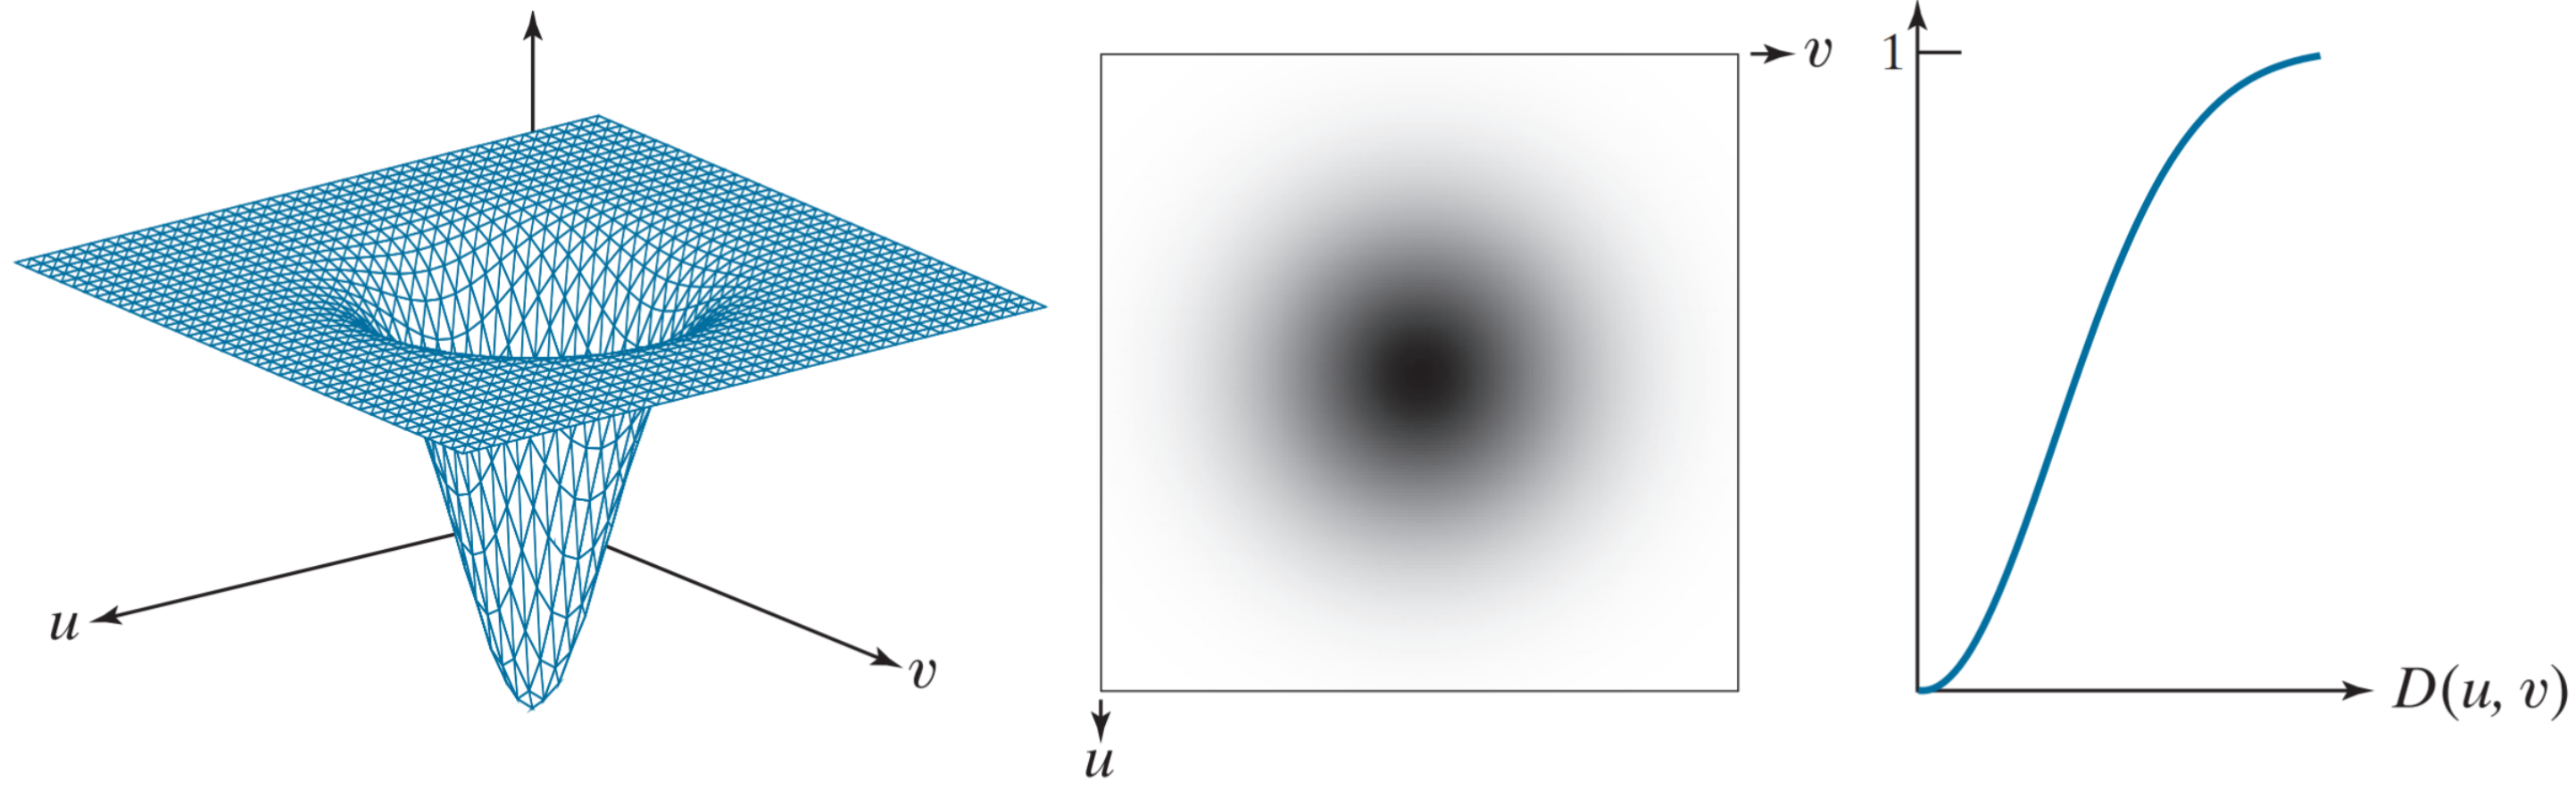
\includegraphics[width=\linewidth]{images/gaussian_high_pass.png}
          \end{figure}
        \end{minipage}

        \begin{equation*}
          H_\text{hp}(u, v) = 1 - e^{-D(u, v)^2/2D_0^2}
        \end{equation*}

    \end{itemize}
\end{itemize}

\subsection*{Fast Fourier Transform (FFT)}

\begin{itemize}
  \item DFT is computationally expensive, with a time complexity of
    $O((MN)^2)$, where M and N are the dimensions of the image
  \item \textbf{Fast Fourier Transform (FFT)} allows the Fourier
    transform to be carried out in a reasonable amount of time
  \item It reduces the amount of time required to complete a Fourier
    transform by a factor of \textbf{100 - 600 times}!
  \item FFT is the reason why Fourier based techniques have gained
    popularity in image processing
\end{itemize}

\subsection*{Spatial vs Frequency Domain}

\begin{itemize}
  \item Similar jobs can be done in both spatial and frequency domains
  \item Filtering in the spatial domain can be easier to understand
  \item Filtering in the frequency domain can be much faster –
    especially for large images
\end{itemize}

\section*{Image Restoration}

Image restoration attempts to restore images that have been degraded.

\begin{itemize}
  \item Identify the degradation process and \textbf{attempt to reverse it}
  \item Similar to image enhancement, but \textbf{more objective}
\end{itemize}

\subsection*{Noise and Images}

The sources of noise in digital images arise during image acquisition
(digitization) and transmission
\begin{itemize}
  \item Imaging sensors can be affected by ambient conditions
  \item Interference can be added to an image during transmission
\end{itemize}

\subsection*{Noise in Images}

We can consider a noisy image to be modeled as follows:

\begin{equation*}
  g(x, y) = f(x, y) + \eta(x, y)
\end{equation*}

(i) $f(x, y) \rightarrow$ original image pixel (ii) $\eta(x, y)
\rightarrow$ the noise term and (iii) $g(x, y) \rightarrow$ resulting
noisy pixel

If we can \textbf{estimate the model} that the noise in an image is
based on, it will help us to figure out \textbf{how to restore the image}.

\subsection*{Mean Filters for Restoration}

\begin{itemize}
  \item \textbf{Arithmetic Mean Filter:} Smooths local variations;
    blurs the image to reduce noise.
    \begin{equation*}
      \hat{f}(x, y) = \frac{1}{mn} \sum_{(s, t) \in S_{xy}} g(s, t)
    \end{equation*}

  \item \textbf{Geometric Mean Filter:} Comparable to the arithmetic
    mean filter, tends to lose less image detail.
    \begin{equation*}
      \hat{f}(x, y) = \left( \prod_{(s, t) \in S_{xy}} g(s, t) \right)^{1/(mn)}
    \end{equation*}

  \item \textbf{Harmonic Mean Filter:} Works well for \textbf{salt
    noise}, but \textbf{fails} for \textbf{pepper noise}. Also does
    well for other kinds of noise, such as \textbf{Gaussian noise}.
    \begin{equation*}
      \hat{f}(x, y) = \frac{mn}{\sum_{(s, t) \in S_{xy}} 1/g(s, t)}
    \end{equation*}

  \item \textbf{Contraharmonic Mean Filter:} Takes a parameter $Q$,
    the \textbf{order} of the filter.
    \begin{itemize}
      \item $Q > 0 \rightarrow$ removes \textbf{pepper noise}
      \item $Q < 0 \rightarrow$ removes \textbf{salt noise}
      \item Wrong value of $Q$ can have drastic results
    \end{itemize}

    \begin{equation*}
      \hat{f}(x, y) = \frac{\sum_{(s, t) \in S_{xy}} g(s, t)^{Q +
      1}}{\sum_{(s, t) \in S_{xy}} g(s, t)^Q}
    \end{equation*}
\end{itemize}

\subsubsection*{Drawbacks with Mean Filtering}

\begin{itemize}
  \item A single pixel with a very \textbf{unrepresentative value}
    can \textbf{significantly affect} the mean value of all the
    pixels in its neighborhood
  \item When the filter neighborhood \textbf{straddles an edge}, the
    filter will \textbf{interpolate new values} for pixels on the
    edge and so will blur that edge; may be a problem if sharp edges
    are required in the output
\end{itemize}

\subsection*{Degradation Models}

Given: (i) corrupted image $g(x, y)$ (ii) some knowledge about the
degradataion function $H$ (iii) some knowledge about the noise $\eta(x, y)$

Objective: obtain an $f(x, y)$ estimate of the original image

\begin{itemize}
  \item \textbf{Spatial domain:} $g(x, y) = h(x, y) * f(x, y) + \eta(x, y)$
  \item \textbf{Frequency domain:} $G(u, v) = H(u, v) * F(u, v) + N(u, v)$
\end{itemize}

Spatial filtering is the method of noise when only additive noise if
present. Enhancement \& restoration become \textbf{almost
indistinguishable disciplines} in this particular case.

\subsection*{Noise Models}

\begin{itemize}
  \item Images are often degraded by \textbf{random noise} with
    \textbf{probabilistic characteristics}
  \item Noise can occur during (i) image capture, (ii) transmission
    or (ii) processing
  \item May be (i) dependent on or (ii) independent of image content
\end{itemize}

\subsubsection*{White Noise}

\begin{itemize}
  \item Simplest noise
  \item Constant power spectrum (its intensity \textbf{does not
    decrease} with \textbf{increasing frequency})
  \item Frequently applied as a \textbf{crude approximation} of image
    noise in most cases
  \item Advantage: simplifies the calculations
\end{itemize}

\subsubsection*{Gaussian Noise}

\begin{equation*}
  p(z) =\frac{1}{\sigma\sqrt{2 \pi}} e^{-(z - \mu)^2/2 \sigma^2}
\end{equation*}

(i) $z \rightarrow$ gray level (ii) $\mu \rightarrow$ mean of average
value of $z$ (iii) $\sigma \rightarrow$ standard deviation of $z$
(iv) 70\% of its values: $[ \mu \pm \sigma ]$ (v) 95\% of its values:
$[ \mu \pm 2\sigma ]$

\begin{itemize}
  \item Very good approximation of noise that occurs in most cases
  \item Probability of the random variable is given by the Gaussian function
\end{itemize}

\subsubsection*{Rayleigh Noise}

\begin{equation*}
  p(z) =
  \begin{cases}
    \frac{2}{b} (z-a) e^{-(z-a)^2/b} & \text{if } z \geq a \\
    0 & \text{otherwise}
  \end{cases}
\end{equation*}

(i) $\mu = a + \sqrt{\pi b / 4}$ (ii) $\sigma^2 = \frac{b(4 - \pi)}{4}$

\subsubsection*{Gamma Noise}

\begin{equation*}
  p(z) =
  \begin{cases}
    \frac{a^b z^{b-1}}{(b-1)!} e^{-az} & \text{if } z \geq a \\
    0 & \text{otherwise}
  \end{cases}
\end{equation*}

(i) $\mu = \frac{b}{a}$ (ii) $\sigma^2 = \frac{b}{a^2}$

\subsubsection*{Exponential Noise}

\begin{equation*}
  p(z) =
  \begin{cases}
    ae^{-az} & \text{if } z \geq 0 \\
    0 & \text{otherwise}
  \end{cases}
\end{equation*}

(i) $\mu = \frac{1}{a}$ (ii) $\sigma^2 = \frac{1}{a^2}$

\subsubsection*{Uniform Noise}

\begin{equation*}
  p(z) =
  \begin{cases}
    \frac{1}{b-a} & \text{if } a \leq z \leq b \\
    0 & \text{otherwise}
  \end{cases}
\end{equation*}

(i) $\mu = \frac{a + b}{2}$ (ii) $\sigma^2 = \frac{(b - a)^2}{12}$

\subsubsection*{Impulse Noise}

Randomly scattered \textbf{white} (\enquote{salt}) or \textbf{black}
(\enquote{pepper}) pixels over the image.

\begin{equation*}
  p(z) =
  \begin{cases}
    P_a & \text{if } z = a \\
    P_b & \text{if } z = b \\
    P_c & \text{otherwise}
  \end{cases}
\end{equation*}

\begin{itemize}
  \item \textbf{Bipolar:} $P_a \neq 0, P_b \neq 0$
  \item \textbf{Unipolar (salt and pepper):} $P_a = 0$ or $P_b = 0$
\end{itemize}

\subsection*{Estimation of Noise Parameters}

\begin{enumerate}
  \item The shape of the histogram identifies the closest PDF match
  \item Get mean \& variance of the gray levels
  \item Use $\mu$ \& $\sigma^2$ to solve for the parameters a \& b
\end{enumerate}

\textbf{Gaussian noise}: mean \& variance only

\textbf{Impulse noise}: the actual probability of occurrence of white
\& black pixels are needed

\subsection*{Order Statistics Filters for Restoration}

The response is based on the \textbf{ordering} of the pixel values in
the image area encompassed by the filter mask.

\begin{itemize}
  \item \textbf{Median Filter:} Removes salt and pepper noise
    \begin{equation*}
      \hat{f}(x, y) = \text{median}_{(a, b) \in S} \left\{ g(x - a, y
      - b) \right\}
    \end{equation*}

  \item \textbf{Max Filter:} Removes pepper noise
    \begin{equation*}
      \hat{f}(x, y) = \max_{(a, b) \in S} \left\{ g(x - a, y - b) \right\}
    \end{equation*}

  \item \textbf{Min Filter:} Removes salt noise
    \begin{equation*}
      \hat{f}(x, y) = \min_{(a, b) \in S} \left\{ g(x - a, y - b) \right\}
    \end{equation*}

  \item \textbf{Midpoint Filter:} Order statistics + averaging; works
    best for Gaussian or uniform noise
    \vspace{-0.1em}
    \begin{equation*}
      \frac{1}{2} \bigg[ \max_{(a, b) \in S} \left\{
        g(x - a, y - b) \right\} + \min_{(a, b) \in S} \left\{ g(x - a,
      y - b) \right\} \bigg]
    \end{equation*}

  \item \textbf{Alpha-trimmed Mean Filter:} Delete the $d/2$ lowest
    and $d/2$ highest gray level values of $g(x - a, y - b)$. Useful
    for situations involving multiple types of noise.

    \begin{equation*}
      \hat{f}(x, y) = \frac{g_r(x, y)}{mn - d}
    \end{equation*}

    $g_r \rightarrow$ sum of the remaining pixel values
\end{itemize}

\subsubsection*{Drawbacks with Order Statistics Filters}

\begin{itemize}
  \item Relatively expensive and complex to compute.
  \item To find the median it is necessary to \textbf{sort all the
    values} in the neighborhood into numerical order
  \item Sorting is relatively slow, even with fast sorting algorithms
    such as \textbf{quicksort}
  \item \textbf{Possible remedy:} When the filter is slid across the
    image, many of the pixels in the window are the same from one
    step to the next; the relative ordering of these with each other
    do not change
\end{itemize}

\subsection*{Adaptive Filtering}

Changing the behavior according to gray level values under the filter mask.

\begin{equation*}
  m_f + \frac{\sigma_f^2}{\sigma_f^2 + \sigma_g^2} (g - m_f)
\end{equation*}

\begin{itemize}
  \item $m_f \rightarrow$ mean under the mask
  \item $\sigma_f^2 \rightarrow$ variance under the mask
    (\enquote{local variance})
  \item $g \rightarrow$ current (grayscale) pixel value
  \item $\sigma_g^2 \rightarrow$ variance of the image
\end{itemize}

Insights:

\begin{itemize}
  \item $\sigma_f^2$ high $\rightarrow$ fraction is close to $1$,
    output is closer to \textbf{original value} ($g$), significant
    details (e.g. edges).

  \item $\sigma_f^2$ low $\rightarrow$ fraction is close to $0$,
    output is closer to \textbf{mean value} ($m_f$), smooths out noise.

  \item $\sigma_g^2$ often unknown; taken as the \textbf{mean} of all
    values of $\sigma_f^2$ in the image.
\end{itemize}

\subsubsection*{Variant}

Pratically, a \textbf{variant} of adaptive filtering is used:

\begin{equation*}
  m_f + \frac{\max \{0, \sigma_f^2 - \sigma_g^2 \}}{\max\{\sigma_f^2
  + \sigma_g^2\}} (g - m_f)
\end{equation*}

Purposes:

\begin{itemize}
  \item Removes salt and pepper noise
  \item Smooths other noise that may not be impulsive
  \item Reduces distortion (e.g. excessive thickening/thinning of boundaries)
\end{itemize}

\subsubsection*{Adaptive Median Filter}

\begin{itemize}
  \item The median filter performs relatively well on \textbf{impulse noise}
    as long as the \textbf{spatial density} of the impulse noise is
    \textbf{not large}
  \item The \textbf{adaptive median filter} can handle much more spatially
    dense impulse noise
  \item It also performs some \textbf{smoothing} for non-impulse noise
  \item Key insight: \textbf{filter size changes} depending on the
    characteristics of the image
\end{itemize}

\textbf{Level A}

\begin{enumerate}
  \item $A_1 = z_\text{med} - z_{min}$
  \item $A_2 = z_\text{med} - z_{max}$
  \item If $A_1 > 0$ and $A_2 < 0$, go to level B
  \item Else increase the window size
  \item If window size $\leq S_\text{max}$, repeat level A
  \item Else output $z_\text{med}$
\end{enumerate}

\textbf{Level B}

\begin{enumerate}
  \item $B_1 = z_\text{xy} - z_\text{min}$
  \item $B_2 = z_\text{xy} - z_\text{max}$
  \item If $B_1 > 0$ and $B_2 < 0$, output $z_\text{xy}$
  \item Else output $z_\text{med}$
\end{enumerate}

\subsection*{Periodic Noise}

\begin{itemize}
  \item Typically arises due to \textbf{electrical or electromagnetic
    interference}
  \item Effect: regular noise patterns in an image
  \item \textbf{Frequency domain techniques} most effective
\end{itemize}

\subsection*{Band-Reject Filters}

Removes a particular range of frequencies from the image

\textbf{Ideal band-reject filter:}

\begin{equation*}
  H(u,v)=
  \begin{cases}
    1 & \text{if } D(u,v) < D_0 - \dfrac{W}{2}\\
    0 & \text{if } D_0 - \dfrac{W}{2} \le D(u,v) \le D_0 + \dfrac{W}{2}\\
    1 & \text{if } D(u,v) > D_0 + \dfrac{W}{2}
  \end{cases}
\end{equation*}

\begin{figure}[H]
  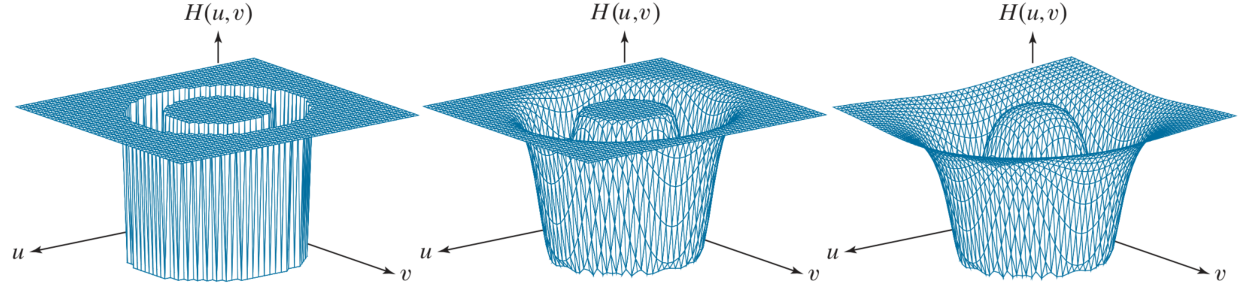
\includegraphics[width=\linewidth]{images/band_reject_filters.png}
  \caption{Ideal, Gaussian and Butterworth band-reject filters}
\end{figure}

\subsection*{Degradation}

$G(u, v) = F(u, v) * H(u, v)$

(i) $G(u, v) \rightarrow$ degraded image (ii) $F(u, v) \rightarrow$
original image (iii) $H(u, v) \rightarrow$ filter (degradation function)

Goal: $G$ and $H$ are known, obtain $F$

\subsubsection*{Inverse Filtering}

Simplest approach to restoration.

\begin{equation*}
  \hat{F}(u, v) = \frac{G(u, v)}{H(u, v)} = F(u, v) + \frac{N(u, v)}{H(u, v)}
\end{equation*}

$N(u, v) \rightarrow$ random function whose Fourier transform is
unknown; we cannotrecover the undegraded image even if $H(u, v)$ is known.

\begin{itemize}
  \item \textbf{Problem:} If $H(u, v)$ approaches 0, $\frac{N(u, v)}{H(u,
    v)}$ dominates the estimate $\hat{F}(u, v)$.
  \item \textbf{Solution:} Limit the analysis to frequencies near the origin.
\end{itemize}

\textbf{Approaches:}

\begin{itemize}
  \item \textbf{Low-pass filtering:} Uses filter $L(u, v)$
    \begin{equation*}
      F(u, v) = \frac{G(u, v)}{H(u, v)}L(u, v)
    \end{equation*}
  \item \textbf{Thresholding:} Using only filter frequencies near the origin
    \begin{equation*}
      F(u, v) =
      \begin{cases}
        \frac{G(u, v)}{H(u, v)} & \text{if } D(u, v) < d \\
        G(u, v) & \text{otherwise}
      \end{cases}
    \end{equation*}
\end{itemize}

\textbf{Weaknesses:}

\begin{itemize}
  \item Inverse filtering is \textbf{not robust} to noise (doesn't
    explicitly handle it)
  \item Easily corrupted by random noise
    \begin{gather*}
      G(u, v) = F(u, v) * H(u, v) + N(u, v) \\
      F(u, v) = \frac{G(u, v) - N(u, v)}{H(u, v)}
    \end{gather*}
  \item The noise can completely dominate the output
\end{itemize}

\subsubsection*{Wiener Filtering}

Aims to minimize the \textbf{mean square error} between the original
image and the restored image.

\begin{equation*}
  \hat{F}(u, v) = \bigg[ \frac{1}{H(u, v)} \frac{|H(u, v)|^2}{|H(u, v)|^2 + K} \bigg] G(u, v)
\end{equation*}

$K \rightarrow$ specified constant

\section*{Segmentation}

Goal: partition the pixels of an image into \textbf{groups} that
strongly correlate with the \textbf{objects} in an image

Typically the \textbf{first step} in any automated computer vision application

\subsection*{Detection of Discontinuities}

\subsubsection*{Point Detection}

The following filter is applied, then the pixels above a certain
threshold are considered points:

\vspace{-0.3cm}
\begin{figure}[H]
  \centering
  \begin{tikzpicture}[%
      filtercell/.style={draw=MaterialBlue900, fill=MaterialBlue50,
      minimum size=1cm, anchor=center}
    ]
    \node[filtercell] (f11) at (0,2) {$-1$};
    \node[filtercell] (f12) at (1,2) {$-1$};
    \node[filtercell] (f13) at (2,2) {$-1$};
    \node[filtercell] (f21) at (0,1) {$-1$};
    \node[filtercell] (f22) at (1,1) {$8$};
    \node[filtercell] (f23) at (2,1) {$-1$};
    \node[filtercell] (f31) at (0,0) {$-1$};
    \node[filtercell] (f32) at (1,0) {$-1$};
    \node[filtercell] (f33) at (2,0) {$-1$};

  \end{tikzpicture}
  \caption{Point detection filter}
\end{figure}

\subsubsection*{Line Detection}

Masks below extract one pixel thick lines running in a particular direction:

\begin{figure}[ht]
  \centering
  % first row
  \begin{subfigure}[t]{0.5\linewidth}
    \centering
    % Horizontal filter
    \begin{tikzpicture}[filtercell/.style={
          draw=MaterialBlue900, fill=MaterialBlue50,
      minimum size=1cm, inner sep=0pt, outer sep=0pt}]
      \foreach \x in {0,1,2}{
        \node[filtercell] at (\x,2) {$-1$};
        \node[filtercell] at (\x,1) {$ 2$};
        \node[filtercell] at (\x,0) {$-1$};
      }
    \end{tikzpicture}
    \subcaption{Horizontal}
  \end{subfigure}%
  \begin{subfigure}[t]{0.48\linewidth}
    \centering
    % Vertical filter
    \begin{tikzpicture}[filtercell/.style={
          draw=MaterialBlue900, fill=MaterialBlue50,
      minimum size=1cm, inner sep=0pt, outer sep=0pt}]
      \foreach \y in {0,1,2}{
        \node[filtercell] at (0,\y) {$-1$};
        \node[filtercell] at (1,\y) {$ 2$};
        \node[filtercell] at (2,\y) {$-1$};
      }
    \end{tikzpicture}
    \subcaption{Vertical}
  \end{subfigure}

  \bigskip  % vertical gap

  % second row
  \begin{subfigure}[t]{0.48\linewidth}
    \centering
    % Diagonal (\) filter
    \begin{tikzpicture}[filtercell/.style={
          draw=MaterialBlue900, fill=MaterialBlue50,
      minimum size=1cm, inner sep=0pt, outer sep=0pt}]
      \node[filtercell] at (0,2) {$-1$};
      \node[filtercell] at (1,2) {$-1$};
      \node[filtercell] at (2,2) {$ 2$};
      \node[filtercell] at (0,1) {$-1$};
      \node[filtercell] at (1,1) {$ 2$};
      \node[filtercell] at (2,1) {$-1$};
      \node[filtercell] at (0,0) {$ 2$};
      \node[filtercell] at (1,0) {$-1$};
      \node[filtercell] at (2,0) {$-1$};
    \end{tikzpicture}
    \subcaption{Diagonal ($+45^\circ$)}
  \end{subfigure}%
  \begin{subfigure}[t]{0.48\linewidth}
    \centering
    % Diagonal (/) filter
    \begin{tikzpicture}[filtercell/.style={
          draw=MaterialBlue900, fill=MaterialBlue50,
      minimum size=1cm, inner sep=0pt, outer sep=0pt}]
      \node[filtercell] at (0,2) {$ 2$};
      \node[filtercell] at (1,2) {$-1$};
      \node[filtercell] at (2,2) {$-1$};
      \node[filtercell] at (0,1) {$-1$};
      \node[filtercell] at (1,1) {$ 2$};
      \node[filtercell] at (2,1) {$-1$};
      \node[filtercell] at (0,0) {$-1$};
      \node[filtercell] at (1,0) {$-1$};
      \node[filtercell] at (2,0) {$ 2$};
    \end{tikzpicture}
    \subcaption{Diagonal ($-45^\circ$)}
  \end{subfigure}

  \caption{Line‐detection filters in four orientations.}
\end{figure}

\subsubsection*{Edge Detection}

An \textbf{edge} is a set of connected pixels that lie on the
boundary between two regions.

\begin{figure}[H]
  \centering
  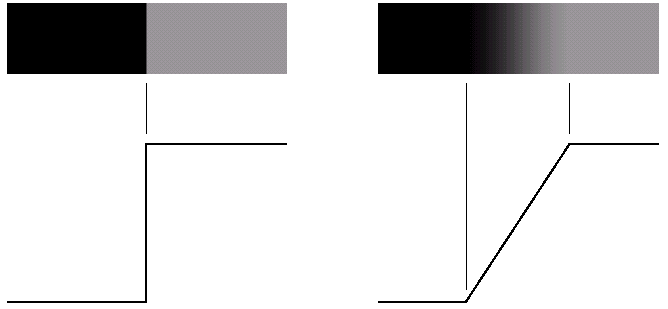
\includegraphics[width=\linewidth]{images/edge_models.png}
  \caption{Two common edge models: ideal (step) and ramp}
\end{figure}

Note: Derivative-based edge detectors are \textbf{extremely sensitive to noise}.

\textbf{Common edge detectors}:

\begin{itemize}

  \item \textbf{Roberts}

    \begin{minipage}{\linewidth}
      \vspace{-0.3cm}
      \begin{figure}[H]
        \centering
        \begin{tikzpicture}[%
            filtercell/.style={draw=MaterialBlue900, fill=MaterialBlue50,
            minimum size=1cm, anchor=center}
          ]
          % G_x
          \node[filtercell] (r111) at (0,1) {$-1$};
          \node[filtercell] (r112) at (1,1) {$0$};
          \node[filtercell] (r121) at (0,0) {$0$};
          \node[filtercell] (r122) at (1,0) {$1$};
          % G_y
          \node[filtercell] (r211) at (3,1) {$0$};
          \node[filtercell] (r212) at (4,1) {$-1$};
          \node[filtercell] (r221) at (3,0) {$1$};
          \node[filtercell] (r222) at (4,0) {$0$};
        \end{tikzpicture}
        \caption{Roberts filters for $G_x$ (left) and $G_y$ (right)}
      \end{figure}
    \end{minipage}

  \item \textbf{Prewitt}

    \begin{minipage}{\linewidth}
      \vspace{-0.3cm}
      \begin{figure}[H]
        \centering
        \begin{tikzpicture}[%
            filtercell/.style={draw=MaterialBlue900, fill=MaterialBlue50,
            minimum size=1cm, anchor=center}
          ]
          % G_x
          \node[filtercell] (p111) at (0,2) {$-1$};
          \node[filtercell] (p112) at (1,2) {$-1$};
          \node[filtercell] (p113) at (2,2) {$-1$};
          \node[filtercell] (p121) at (0,1) {$0$};
          \node[filtercell] (p122) at (1,1) {$0$};
          \node[filtercell] (p123) at (2,1) {$0$};
          \node[filtercell] (p131) at (0,0) {$1$};
          \node[filtercell] (p132) at (1,0) {$1$};
          \node[filtercell] (p133) at (2,0) {$1$};
          % G_y
          \node[filtercell] (p211) at (4,2) {$-1$};
          \node[filtercell] (p212) at (5,2) {$0$};
          \node[filtercell] (p213) at (6,2) {$1$};
          \node[filtercell] (p221) at (4,1) {$-1$};
          \node[filtercell] (p222) at (5,1) {$0$};
          \node[filtercell] (p223) at (6,1) {$1$};
          \node[filtercell] (p231) at (4,0) {$-1$};
          \node[filtercell] (p232) at (5,0) {$0$};
          \node[filtercell] (p233) at (6,0) {$1$};
        \end{tikzpicture}
        \caption{Prewitt filters for $G_x$ (left) and $G_y$ (right)}
      \end{figure}
    \end{minipage}

  \item \textbf{Sobel}

    \begin{minipage}{\linewidth}
      \vspace{-0.3cm}
      \begin{figure}[H]
        \centering
        \begin{tikzpicture}[%
            filtercell/.style={draw=MaterialBlue900, fill=MaterialBlue50,
            minimum size=1cm, anchor=center}
          ]
          % G_x
          \node[filtercell] (s111) at (0,2) {$-1$};
          \node[filtercell] (s112) at (1,2) {$0$};
          \node[filtercell] (s113) at (2,2) {$1$};
          \node[filtercell] (s121) at (0,1) {$-2$};
          \node[filtercell] (s122) at (1,1) {$0$};
          \node[filtercell] (s123) at (2,1) {$2$};
          \node[filtercell] (s131) at (0,0) {$-1$};
          \node[filtercell] (s132) at (1,0) {$0$};
          \node[filtercell] (s133) at (2,0) {$1$};
          % G_y
          \node[filtercell] (s211) at (4,2) {$-1$};
          \node[filtercell] (s212) at (5,2) {$-2$};
          \node[filtercell] (s213) at (6,2) {$-1$};
          \node[filtercell] (s221) at (4,1) {$0$};
          \node[filtercell] (s222) at (5,1) {$0$};
          \node[filtercell] (s223) at (6,1) {$0$};
          \node[filtercell] (s231) at (4,0) {$1$};
          \node[filtercell] (s232) at (5,0) {$2$};
          \node[filtercell] (s233) at (6,0) {$1$};
        \end{tikzpicture}
        \caption{Sobel filters for $G_x$ (left) and $G_y$ (right)}
      \end{figure}
    \end{minipage}

  \item \textbf{Laplacian of Gaussian:} The \textbf{Laplacian} is typically not used by itself as it is very sensitive to noise; so we combine it with a smoothing operator (Gaussian). This is also known as the \textbf{Mexican hat} filter.

    \begin{minipage}{\linewidth}
      \vspace{-0.3cm}
      \begin{figure}[H]
        \centering
        \begin{tikzpicture}[%
            filtercell/.style={draw=MaterialBlue900, fill=MaterialBlue50,
            minimum size=1cm, anchor=center}
          ]
          % Row y=4
          \node[filtercell] at (0,4) {$0$};
          \node[filtercell] at (1,4) {$0$};
          \node[filtercell] at (2,4) {$-1$};
          \node[filtercell] at (3,4) {$0$};
          \node[filtercell] at (4,4) {$0$};
          % Row y=3
          \node[filtercell] at (0,3) {$0$};
          \node[filtercell] at (1,3) {$-1$};
          \node[filtercell] at (2,3) {$-2$};
          \node[filtercell] at (3,3) {$-1$};
          \node[filtercell] at (4,3) {$0$};
          % Row y=2
          \node[filtercell] at (0,2) {$-1$};
          \node[filtercell] at (1,2) {$-2$};
          \node[filtercell] at (2,2) {$16$};
          \node[filtercell] at (3,2) {$-2$};
          \node[filtercell] at (4,2) {$-1$};
          % Row y=1
          \node[filtercell] at (0,1) {$0$};
          \node[filtercell] at (1,1) {$-1$};
          \node[filtercell] at (2,1) {$-2$};
          \node[filtercell] at (3,1) {$-1$};
          \node[filtercell] at (4,1) {$0$};
          % Row y=0
          \node[filtercell] at (0,0) {$0$};
          \node[filtercell] at (1,0) {$0$};
          \node[filtercell] at (2,0) {$-1$};
          \node[filtercell] at (3,0) {$0$};
          \node[filtercell] at (4,0) {$0$};
        \end{tikzpicture}
        \caption{Laplacian‐of‐Gaussian (LoG) filter}
      \end{figure}
    \end{minipage}

    \begin{minipage}{\linewidth}
      \begin{figure}[H]
        \centering
        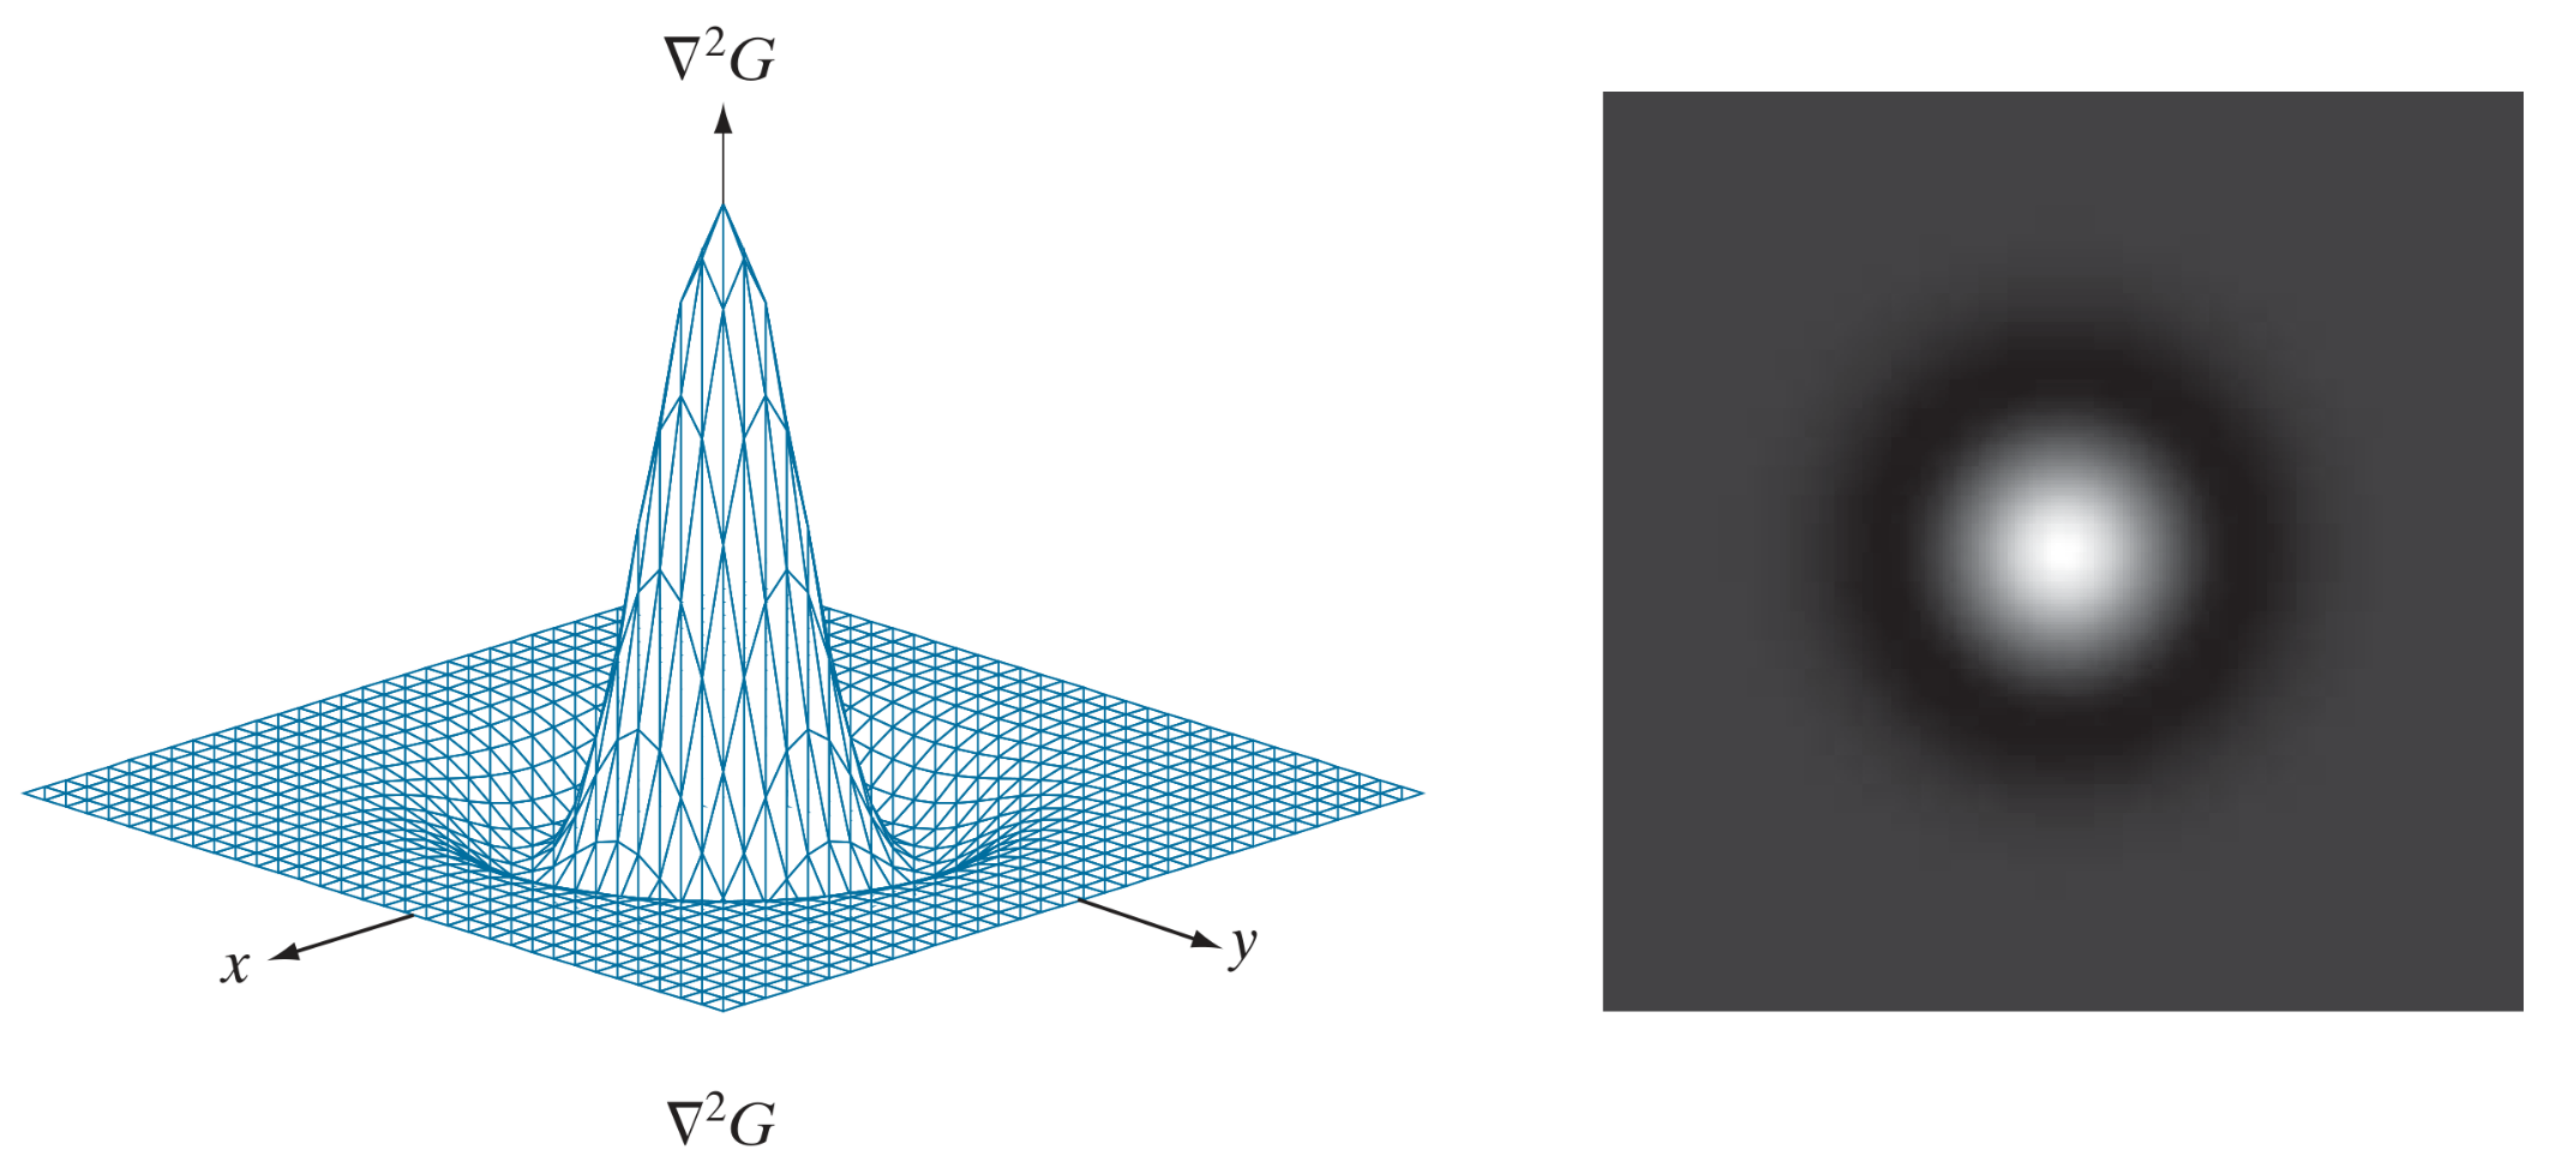
\includegraphics[width=\linewidth]{images/laplacian_of_gaussian.png}
        \caption{Plot of the Mexican hat filter}
      \end{figure}
    \end{minipage}
\end{itemize}

\section*{Thresholding}

Also known as \textbf{binarization}; grayscale $\rightarrow$ binary
image, where each pixel is either black or white

\section*{Single Value Thresholding}

\begin{equation*}
  g(x,y) =
  \begin{cases}
    1, & \text{if } f(x,y) > T,\\
    0, & \text{if } f(x,y) \le T.
  \end{cases}
\end{equation*}

\subsection*{Basic Global Thresholding}

Partitions the \textbf{histogram} of an image using a single global
threshold; success depends on how well the histogram can be separated
into two distinct peaks.

\begin{algorithm}[ht]
  \SetAlgoLined
  \DontPrintSemicolon
  Select an initial estimate for $T$ (typically the average grey
  level in the image)\;
  \Repeat{\textnormal{the difference in} $T$ \textnormal{in
      successive iterations is less than
  a predefined limit} $T_{\infty}$}{
    Segment the image using $T$ to produce two groups of pixels:
    $G_{1}$ consisting of pixels with grey levels $>T$ and $G_{2}$
    consisting pixels with grey levels $\le T$\;
    Compute the average grey levels of pixels in $G_{1}$ to give
    $\mu_{1}$ and $G_{2}$ to give $\mu_{2}$\;
    Compute a new threshold value: $T = (\mu_{1} + \mu_{2})/2$\;
  }
  \caption{Iterative threshold selection}
\end{algorithm}

\subsection*{Challenges}

\begin{itemize}

  \item Single value thresholding only works for \textbf{bimodal}
    histograms. Images with other kinds of histograms need more than
    one threshold.

    \begin{figure}[H]
      \centering
      \includegraphics[width=\linewidth]{images/thresholding_histogram.png}
      \caption{Thresholding on bimodal vs. multimodal histograms}
    \end{figure}

  \item Uneven illumination can be a problem for single value thresholding.
\end{itemize}

\subsection*{Adaptive Thresholding}

\begin{itemize}
  \item For handling situations in which single value thresholding will not work
  \item Divide an image into sub images and threshold these individually
  \item Since the threshold for each pixel depends on its location within an image this technique is said to \textbf{adaptive}
\end{itemize}


\section*{Morphological Processing}

\textbf{Morphological image processing} (or morphology) describes a
range of image processing techniques that deal with the shape (or
morphology) of features in an image.

Morphological operations are typically applied to remove
imperfections introduced during segmentation, and so typically
operate on bi-level images

\subsection*{Structuring Elements, Hits and Fits}

Small binary image which defines the shape of the operation, similar
to a convolution kernel.

Structuring elements can be of any shape and size, typically we use
rectangular images with origin at the \textbf{middle pixel}.

\begin{figure}[H]
  \centering
  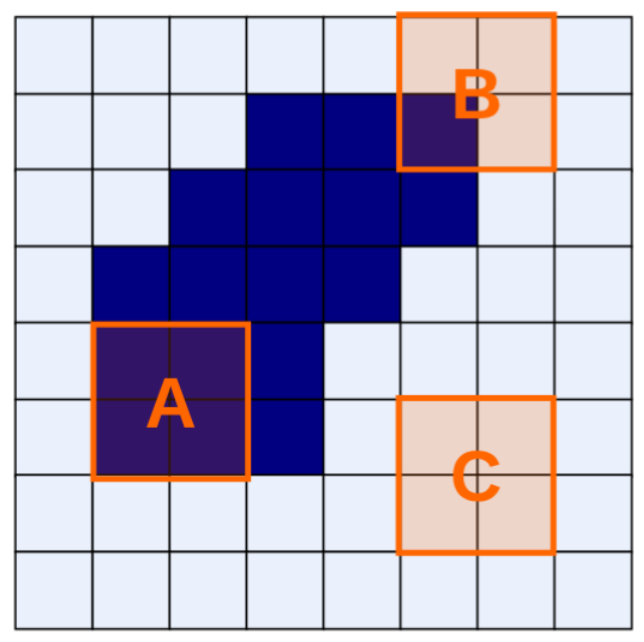
\includegraphics[width=0.5\linewidth]{images/hits_and_fits.png}
  \caption{$A \rightarrow$ fit, $B \rightarrow$ hit, $C \rightarrow$ miss}
\end{figure}

\subsection*{Erosion}

$f \ominus s \rightarrow$ erosion of image $f$ by structuring element $s$.

$s$ is positioned with origin at $(x, y)$ and the new pixel value becomes:

\begin{equation*}
  g(x, y) =
  \begin{cases}
    1 & \text{if } s \text{ fits } f\\
    0 & \text{otherwise}.
  \end{cases}
\end{equation*}

\begin{figure}[H]
  \centering
  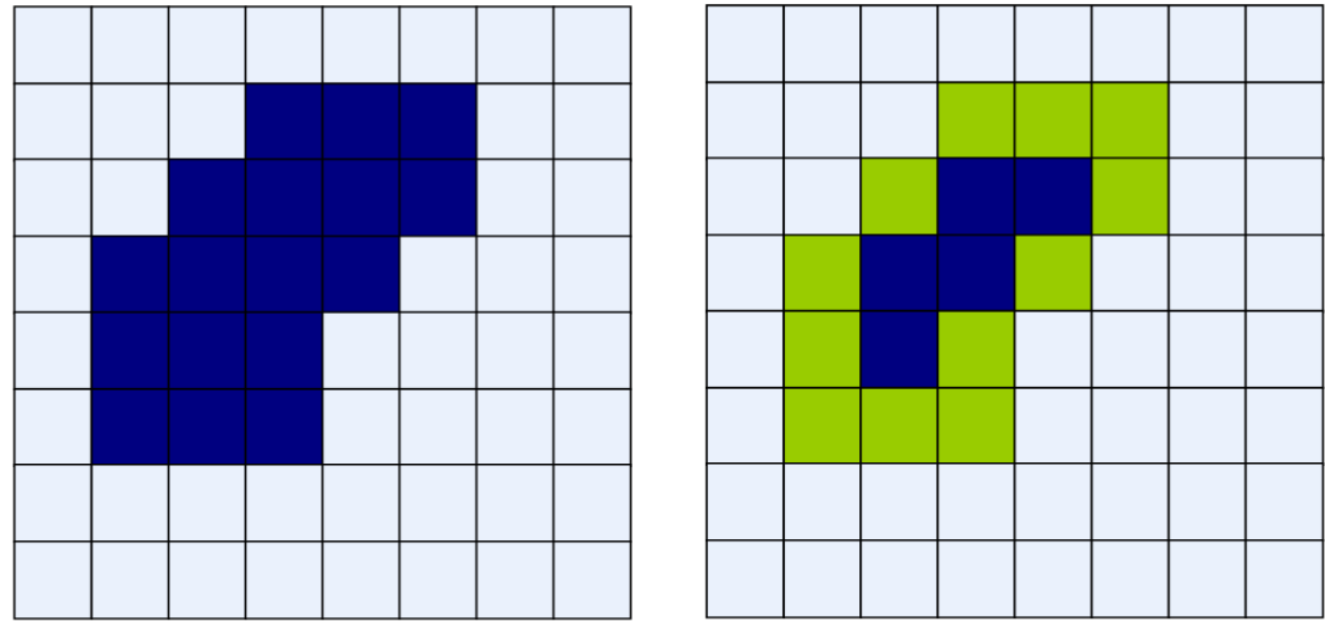
\includegraphics[width=\linewidth]{images/erosion.png}
  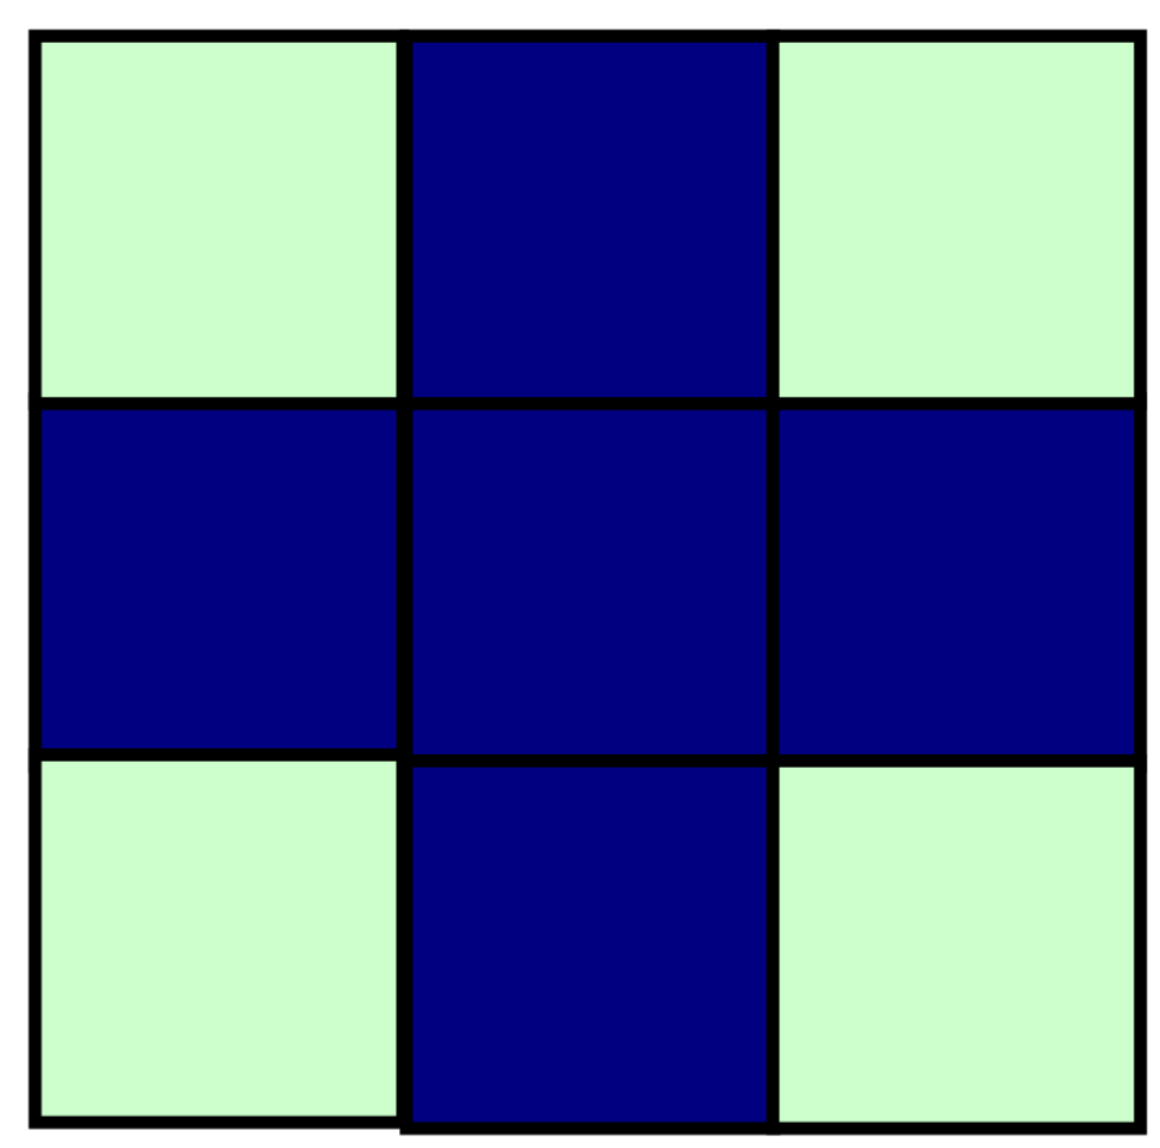
\includegraphics[width=0.18\linewidth]{images/erosion_structuring_element.png}
  \caption{Erosion of a binary image with a plus shaped structuring element; note: \textbf{the boundary shrinks}!}
\end{figure}

\subsubsection*{Applications}

\begin{itemize}
  \item Erosion separates \textbf{joined objects}.

    \begin{minipage}{\linewidth}
      \begin{figure}[H]
        \centering
        \includegraphics[width=0.7\linewidth]{images/erosion_joined_objects.png}
      \end{figure}
    \end{minipage}

  \item Erosion removes \textbf{extrusions}.

    \begin{minipage}{\linewidth}
      \begin{figure}[H]
        \centering
        \includegraphics[width=0.7\linewidth]{images/erosion_extrusions.png}
      \end{figure}
    \end{minipage}
\end{itemize}    

\subsection*{Dilation}

$f \oplus s \rightarrow$ dilation of image $f$ by structuring element $s$.

$s$ is positioned with origin at $(x, y)$ and the new pixel value becomes:

\begin{equation*}
  g(x, y) =
  \begin{cases}
    1 & \text{if } s \text{ hits } f\\
    0 & \text{otherwise}.
  \end{cases}
\end{equation*}

\begin{figure}[H]
  \centering
  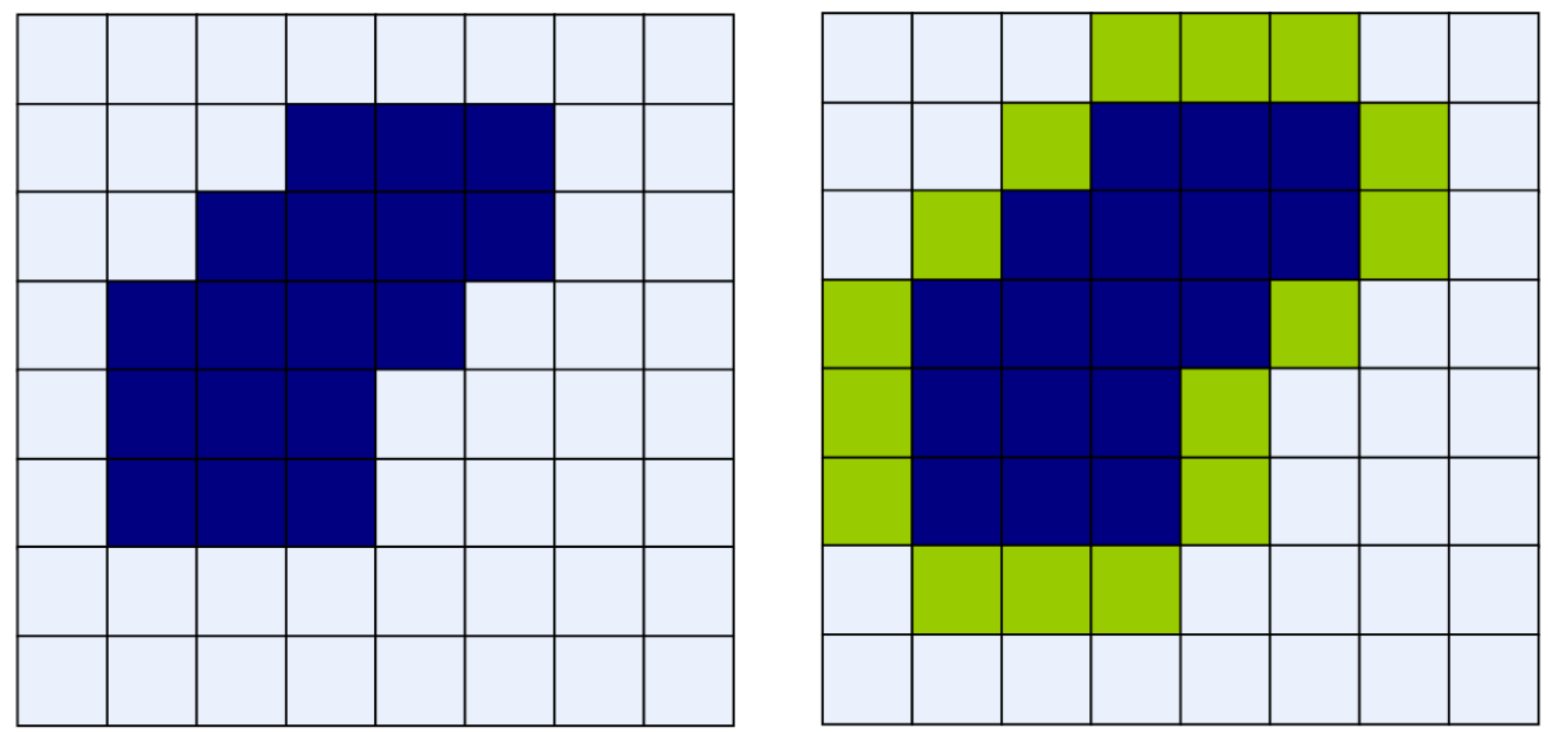
\includegraphics[width=\linewidth]{images/dilation.png}
  \includegraphics[width=0.18\linewidth]{images/dilation_structuring_element.png}
  \caption{Dilation of a binary image with a plus shaped structuring element; note: \textbf{the boundary expands}!}
\end{figure}

\subsubsection*{Applications}

\begin{itemize}
  \item Dilation can \textbf{repair breaks}

    \begin{minipage}{\linewidth}
      \begin{figure}[H]
        \centering
        \includegraphics[width=0.7\linewidth]{images/dilation_repair_breaks.png}
      \end{figure}
    \end{minipage}

  \item Dilation can repair \textbf{intrusions}

    \begin{minipage}{\linewidth}
      \begin{figure}[H]
        \centering
        \includegraphics[width=0.7\linewidth]{images/dilation_repair_intrusions.png}
      \end{figure}
    \end{minipage}
\end{itemize}
  

\subsection*{Opening}

\textbf{Compound operation} of erosion followed by dilation. Separates objects while preserving their size.

\begin{equation*}
  f \circ s = (f \ominus s) \oplus s
\end{equation*}

\begin{figure}[H]
  \centering
  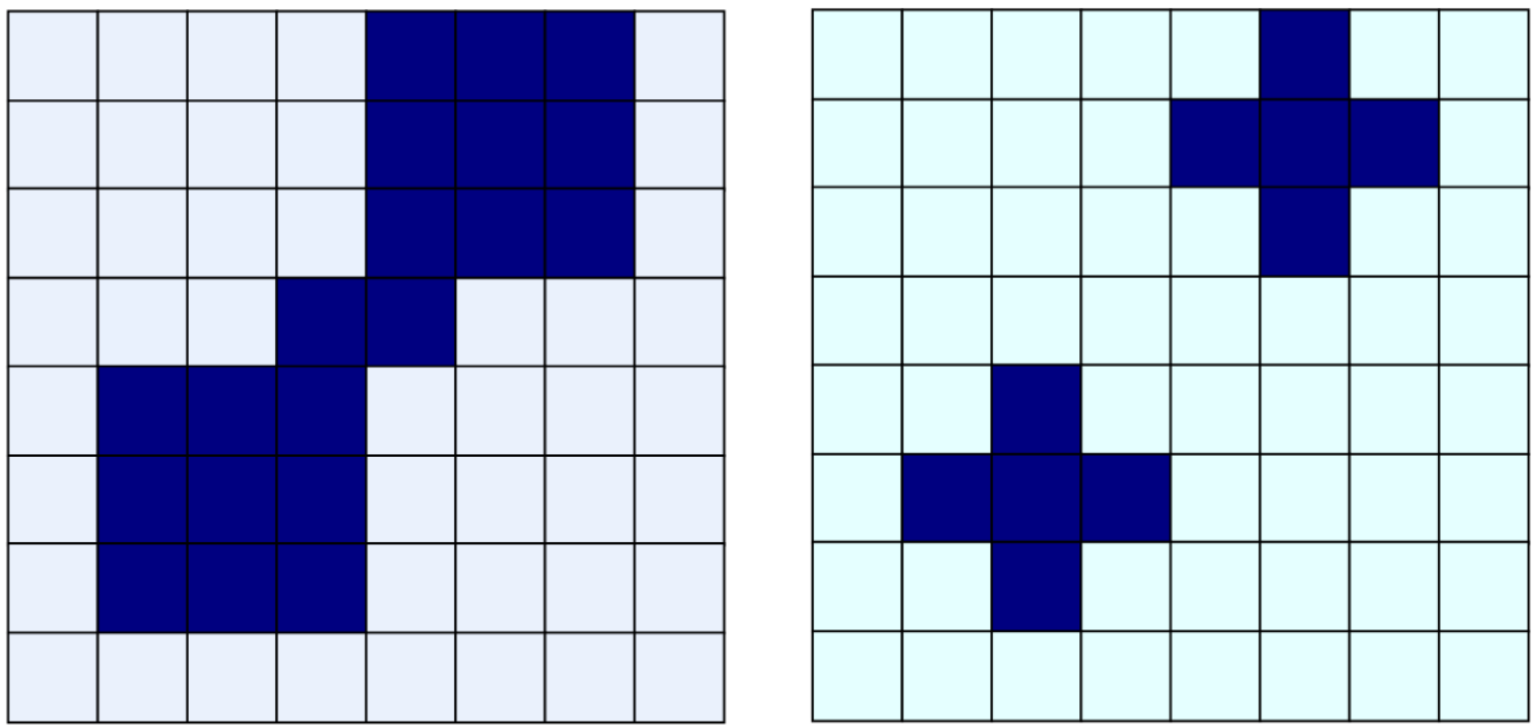
\includegraphics[width=\linewidth]{images/opening.png}
  \includegraphics[width=0.18\linewidth]{images/opening_structuring_element.png}
  \caption{Opening of a binary image with a plus shaped structuring element}
\end{figure}

\subsection*{Closing}

\textbf{Compound operation} of dilation followed by erosion. Fills small holes while preserving the size of objects.

\begin{equation*}
  f \bullet s = (f \oplus s) \ominus s
\end{equation*}

\begin{figure}[H]
  \centering
  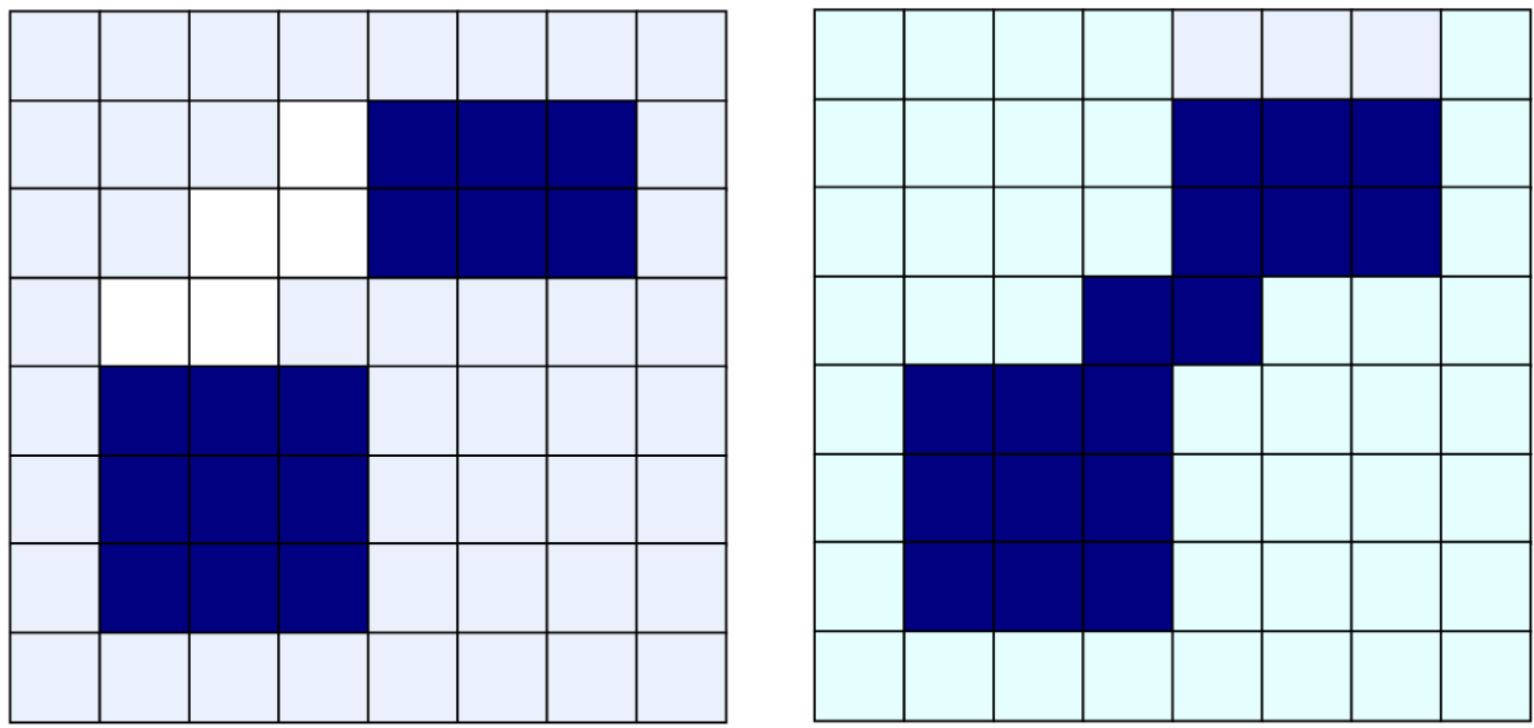
\includegraphics[width=\linewidth]{images/closing.png}
  \includegraphics[width=0.18\linewidth]{images/closing_structuring_element.png}
  \caption{Closing of a binary image with a plus shaped structuring element}
\end{figure}

\textbf{Note}: \enquote{Morphological open-close} is a fairly common operation, which is simply \textbf{opening followed by closing}.

\subsection*{Region Filling}

\textbf{Goal:} Given a pixel inside a boundary, attempt to fill the boundary with \textbf{object pixels} (1's).

\begin{equation*}
  X_k = (X_{k-1} \oplus B) \cap A^c
\end{equation*}

$k = 1, 2, \ldots 3$

(i) $X_0 \rightarrow$ simply the starting point inside the boundary, (ii) $B \rightarrow$ simple structuring element and (iii) $A^c \rightarrow$ complement of A

Equation's applied repeatedly until $X_k$ is equal to $X_{k-1}$

\begin{figure}[H]
  \centering
  \includegraphics[width=\linewidth]{images/region_filling.png}
  \caption{Region filling example}
\end{figure}

\subsubsection*{Applications}
\begin{itemize}
  \item Forensic and biometric fingerprint enhancement: filling spurious gaps in binarized fingerprint images, ensuring continuous ridge structures
  \item Filling in concavities in CT images (such as pleural lesions and eliminate internal cavities caused by respiratory motion specifically in pulmonary CT images) prior to segmentation
\end{itemize}

\subsection*{Boundary Extraction}

The boundary is simply given by:

\begin{equation*}
  \beta(A) = A - A \ominus B
\end{equation*}

\textbf{Intuition:} $A \ominus B$ removes the boundary of $A$ by eroding it with $B$, and then we subtract the eroded image from the original image to get the boundary.

\begin{figure}[H]
  \centering
  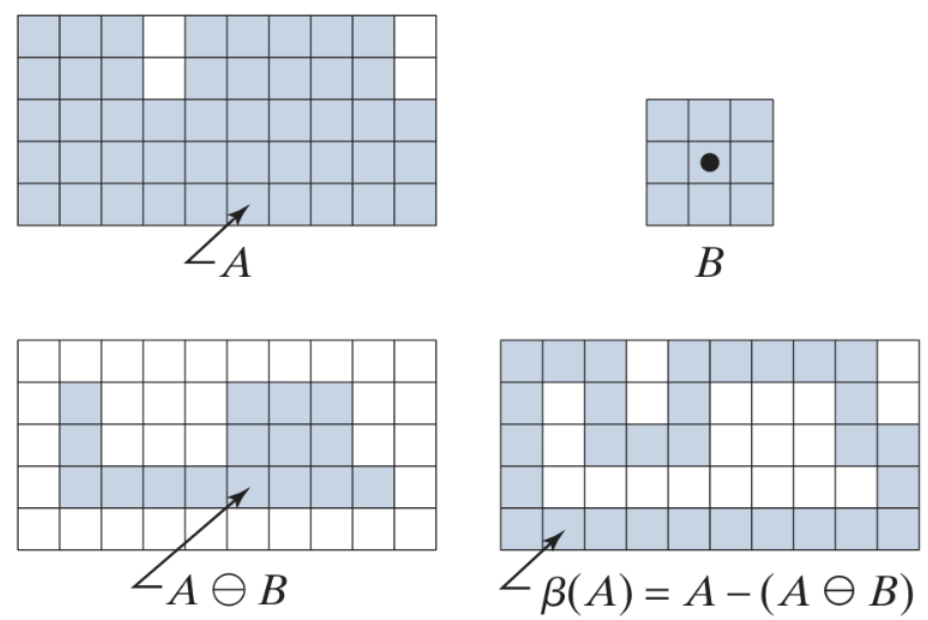
\includegraphics[width=\linewidth]{images/boundary_extraction.png}
  \caption{Boundary extraction example}
\end{figure}

\subsubsection*{Applications}

\begin{itemize}
  \item Optical Character Recognition (OCR) preprocessing: to delineate the contours of text characters, enabling accurate segmentation of connected characters before recognition
  \item Isolating inner and outer boundaries of blood vessel walls in vascular images; useful for measuring arterial lumen and wall thickness
\end{itemize}

\section*{Representation \& Description}

Two ways of representing region:

\begin{itemize}
  \item \textbf{Representation:} in terms of its external
    characteristics (its boundary):
    focus on shape characteristics
  \item \textbf{Description:} in terms of its internal
    characteristics (its region): focus
    on regional properties, e.g., color, texture
\end{itemize}

\subsection*{Sensitivity}

Features selected as descriptors should be as \textbf{insensitive} as
possible to: (i) size, (ii) translation and (iii) rotation

\subsection*{Representation}

\begin{itemize}
  \item Segmentation techniques yield raw data in the form of:
    (i) pixels along a boundary or (ii) pixels contained in a region
  \item These data sometimes are used directly to obtain \textbf{descriptors}
  \item Useful data (descriptors) are extracted from the raw data
    to reduce the amount of data to be processed
\end{itemize}

\subsubsection*{Chain Codes}

Based on the \textbf{4- or 8-connectivity of pixels}, a chain code is a
sequence of directions that describes the boundary of a region.

Usually unacceptable because:

\begin{itemize}
  \item \textbf{Length:} The resulting chain of codes tends to be quite long
  \item \textbf{Sensitivity to Noise:} Small disturbances along the
    boundary due to (i) noise or (ii) imperfect segmentation cause
    changes in the code that may not be related to the shape of the boundary
\end{itemize}

\textbf{Solution:} Resample the boundary by selecting larger grid spacing.
Different grid can generate different chain codes.

\begin{figure}[H]
  \centering
  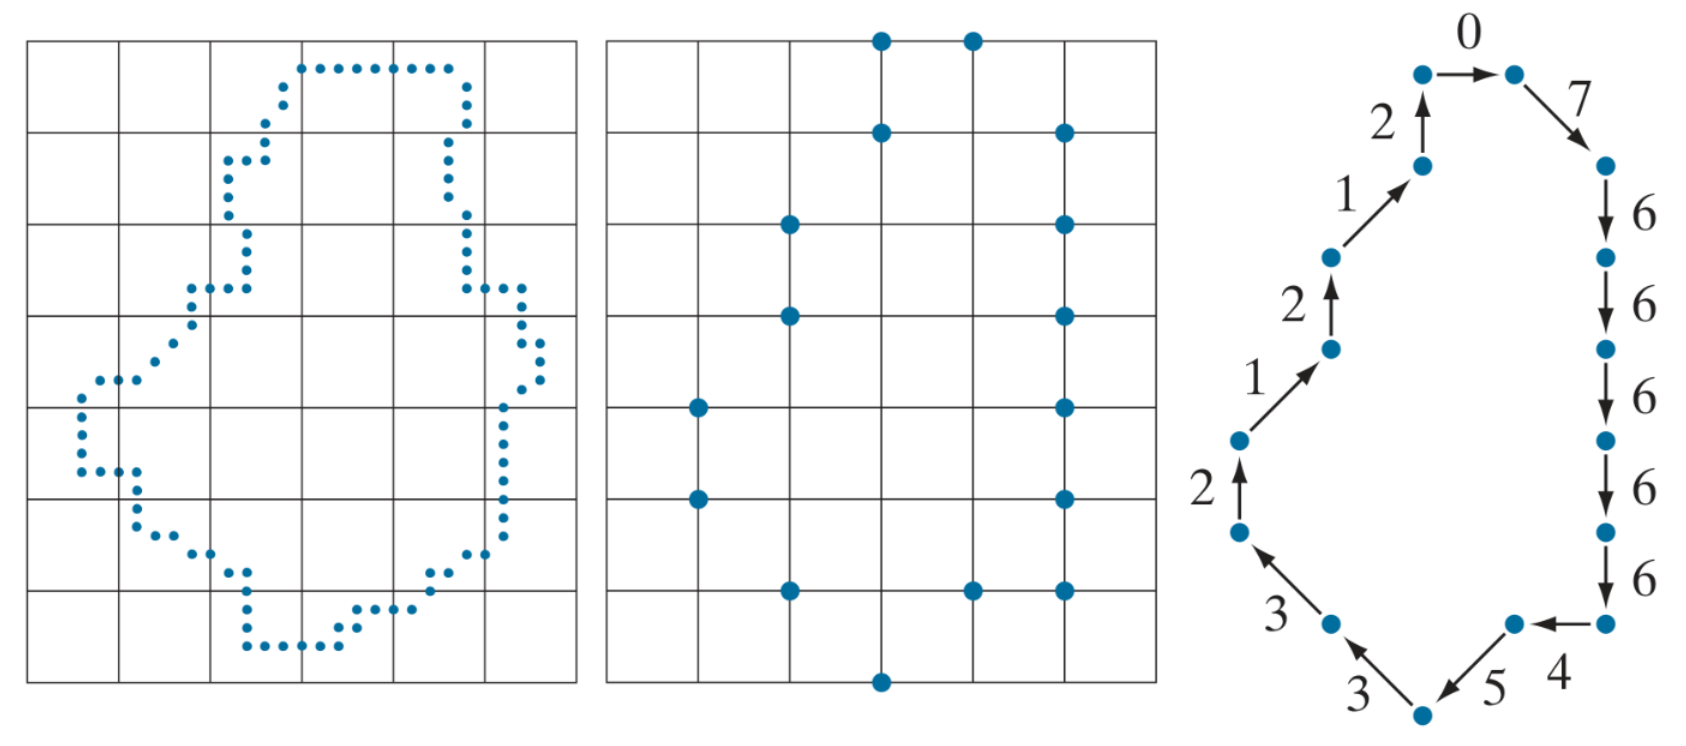
\includegraphics[width=\linewidth]{images/chain_code.png}
  \caption{Resampling to a larger grid, then using 8-neighbor chain code}
\end{figure}

\subsubsection*{Polygonal Approximation}

\begin{itemize}
  \item Boundary can be approximated with arbitrary accuracy by a polygon
  \item Try to capture the \enquote{essence} of the boundary shape
    with the fewest possible polygonal segments
  \item \textbf{Minimum Perimeter Polygon (MPP):} One of the most efficient ways
  \item Not trivial and time consuming
\end{itemize}

\begin{figure}[H]
  \centering
  \includegraphics[width=\linewidth]{images/polygonal_approximation.png}
  \caption{Minimum Perimeter Polygon (MPP) obtained by allowing the
  boundary to shrink to the grid}
\end{figure}

\subsubsection*{Splitting Techniques}

\begin{enumerate}

  \item Find the major axis
  \item Find minor axes which is perpendicular to major axis and has
    distance greater than a threshold
  \item Repeat until we can't split anymore
\end{enumerate}

\begin{figure}[H]
  \centering
  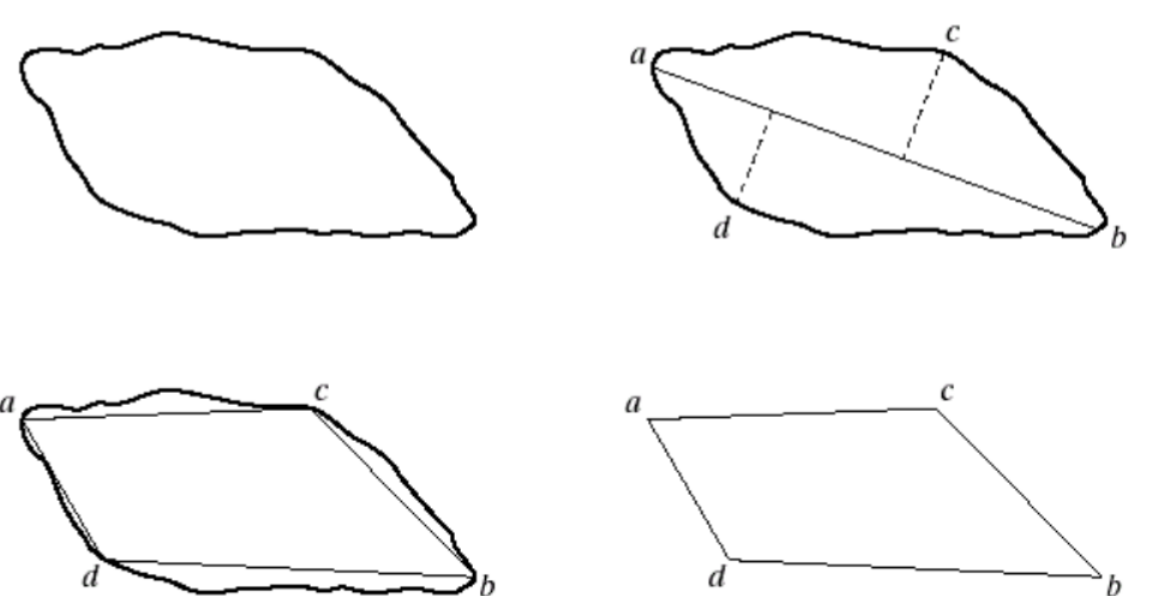
\includegraphics[width=\linewidth]{images/splitting.png}
  \caption{Dividing the boundary based on extreme points, then
  joining them using segments}
\end{figure}

\subsubsection*{Signatures}

\textbf{Signature} is a 1-D functional representation of a 2-D boundary.

\begin{itemize}
  \item Simplest technique: plot the distance of the boundary from
    the centroid ($r$) to the boundary as a function of angle ($\theta$)
  \item Samples are taken at regular intervals of angle $\theta$
\end{itemize}

\begin{figure}[H]
  \centering
  \includegraphics[width=\linewidth]{images/signatures.png}
  \caption{Signatures of circular vs square boundaries}
\end{figure}

\begin{figure}[H]
  \centering
  \includegraphics[width=\linewidth]{images/binary_regions_signatures.png}
  \caption{Signatures of some irregular binary regions}
\end{figure}

\subsubsection*{Convex Hull/Boundary Segments}

A convex hull $H$ of an arbitrary set $S$ is the \textbf{smallest
convex set} containing $S$.

The set difference $H - S$ is called the \textbf{convex deficiency} $D$ of $S$.

\begin{figure}[H]
  \centering
  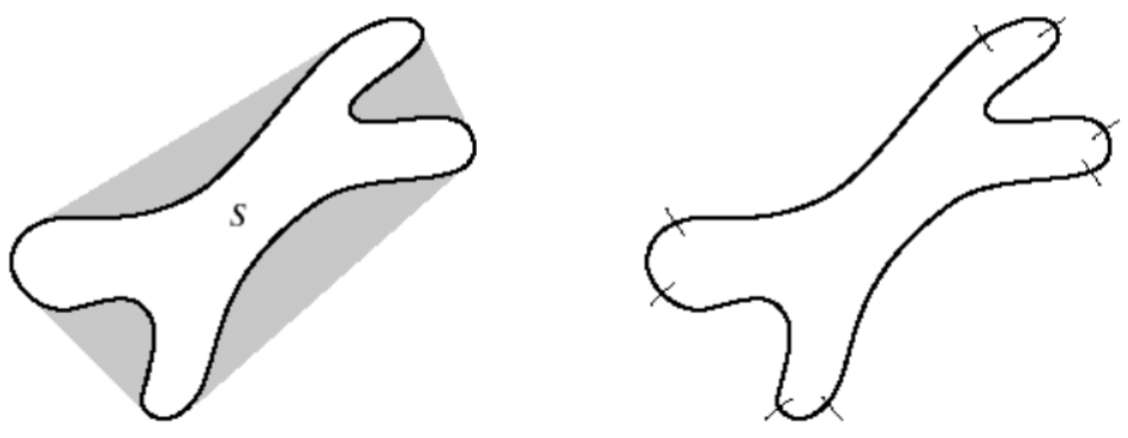
\includegraphics[width=\linewidth]{images/convex_hull_boundary_segments.png}
  \caption{Convex hull of a region (left), partitioned boundary (right)}
\end{figure}

\subsubsection*{Skeletonization}

A \textbf{skeleton} of a region is a thin version of the region. Also
known as \textbf{medial axis}.

\begin{figure}[H]
  \centering
  \includegraphics[width=\linewidth]{images/skeletonization.png}
  \caption{Process of skeletonizing a region; (i) the dashed lines
    represent the skeleton (ii) the circles are \enquote{maximum
    disks}, the largest disks centered at any point inside the region
  and contained in the region.}
\end{figure}

\begin{figure}[H]
  \centering
  \includegraphics[width=\linewidth]{images/skeleton_handwritten.png}
  \caption{Skeleton of binarized handwritten characters}
\end{figure}

\subsection*{Boundary Descriptors}

\subsubsection*{Length of a Boundary}

The \textbf{number of pixels along a boundary} gives a rough
approximation of its length

\subsubsection*{Diameter}

\begin{equation*}
  \text{Diam}(B) = \max_{i, j}[D(p_i, p_j)]
\end{equation*}

$D \rightarrow$ distance measure, $p_i, p_j \rightarrow$ points on boundary $B$.

\subsubsection*{Eccentricity}

Ratio of the \textbf{major axis} to the \textbf{minor axis}:

\begin{itemize}
  \item \textbf{Major axis:} Line connecting the two extreme points
    that comprise the diameter
  \item \textbf{Minor axis:} Line perpendicular to the major axis
    that passes through the centroid of the region
\end{itemize}

\subsection*{Regional Descriptors}

\subsubsection*{Simple Descriptors}

\begin{itemize}
  \item \textbf{Area:} The number of pixels in the region
  \item \textbf{Perimeter:} Length of the boundary
  \item \textbf{Compactness:} $\text{Comp} =
    \frac{\text{Perimeter}^2}{\text{Area}}$

\end{itemize}

\subsubsection*{Topological Descriptors}

\begin{itemize}
  \item \textbf{Euler number:} $\chi = C - H$, where $C$ is the
    number of connected components and $H$ is the number of holes
\end{itemize}

\begin{figure}[H]
  \centering
  \includegraphics[width=\linewidth]{images/euler_numbers.png}
  \caption{Two regions with Euler number 0 and -1 respectively}
\end{figure}

\section*{Color Image Processing}

Light is made up of a spectrum of \textbf{electromagnetic radiation},
each wavelength having its own color.

The colors that humans and most animals perceive in an object are
determined by the nature of the light reflected from the object

For example, green objects reflect light with wave lengths primarily
in the range of 500 – 570 nm while absorbing most of the energy at
other wavelengths

Chromatic light spans the electromagnetic spectrum from approximately
400 to 700 nm

Human color vision is achieved through 6 to 7 million cones in each eye

\subsection*{Quality of a Chromatic Light Source}

\begin{itemize}
  \item \textbf{Radiance:} the total amount of energy that flows from
    the light source (measured in watts)
  \item \textbf{Luminance:} the amount of energy an observer
    perceives from the light source (measured in lumens)
  \item \textbf{Brightness:} a subjective (practically unmeasurable)
    notion that embodies the intensity of light
\end{itemize}

\subsection*{CIE Chromaticity Diagram}

\begin{itemize}
  \item Specifying colors systematically can be achieved using the
    CIE chromacity diagram
  \item On this diagram the \textbf{x-axis} represents the
    \textbf{proportion of red} and the \textbf{y-axis} represents the
    \textbf{proportion of green} used
  \item The proportion of blue used in a color is calculated as: $z
    = 1 – (x + y)$
\end{itemize}

\begin{figure}[H]
  \centering
  \includegraphics[width=0.8\linewidth]{images/cie_chromaticity_diagram.png}
  \caption{CIE Chromaticity Diagram Broken Down into Regions}
\end{figure}

\subsubsection*{Properties}

\begin{itemize}
  \item Any color located on the boundary of the chromacity chart is
    fully saturated
  \item The point of equal energy has equal amounts of each color
    and is the CIE standard for pure white
  \item Any straight line joining two points in the diagram defines
    all of the different colors that can be obtained by combining
    these two colors additively
  \item The above can be easily extended to three points
  \item This means the entire color range cannot be displayed based
    on any three colors
  \item The \textbf{triangle} shows the typical color gamut produced
    by RGB monitors
  \item The \textbf{strange shape} is the gamut achieved by high
    quality color printers
\end{itemize}

\begin{figure}
  \centering
  \includegraphics[width=0.8\linewidth]{images/cie_triangle.png}
  \caption{CIE Chromaticity Diagram with RGB Triangle and Printer Gamut}
\end{figure}

\subsection*{Color Models}

\subsubsection*{RGB Color Model}

\begin{itemize}
  \item Based on the Cartesian coordinate system
  \item Each color appears in its primary spectral components of
    \textcolor{MaterialRed900}{red},
    \textcolor{MaterialGreen900}{green}, and \textcolor{MaterialBlue900}{blue}

  \item RGB values are at 3 corners
  \item Cyan magenta and yellow are at \textbf{other three corners}
  \item Black is at the origin
  \item White is the corner \textbf{furthest from the origin}
  \item Different colors are points on or inside the cube represented
    by RGB vectors
\end{itemize}

\begin{minipage}{\linewidth}
  \begin{figure}[H]
    \centering
    \includegraphics[width=\linewidth]{images/rgb_cube.png}
    \caption{RGB Color Cube}
  \end{figure}
\end{minipage}

\textbf{Properties:}

\begin{itemize}

  \item Images represented in the RGB color model consist of three
    component images – one for each primary color
  \item When fed into a monitor these images are combined to create a
    composite color image
  \item The number of bits used to represent each pixel is referred
    to as the \textbf{color depth}
  \item A 24-bit image is often referred to as a \textbf{full-color image} as
    it allows = 16,777,216 colors
\end{itemize}

\subsubsection*{HSI Color Model}

\textbf{Motivation:}

\begin{itemize}
  \item RGB is useful for hardware implementations related to the way
    in which the human visual system works, but \textbf{not very intuitive}
  \item People tend to use \textbf{hue, saturation and brightness}
  \item RGB is great for color generation, but HSI is great for color
    description
\end{itemize}

\textbf{Model Description:}

\begin{itemize}
  \item \textbf{Hue:} A color attribute that \textbf{describes a pure color}
    (pure yellow, orange or red)
  \item \textbf{Saturation:} Gives a measure of how much a pure
    color is \textbf{diluted with white light}
  \item \textbf{Intensity:} Brightness is nearly impossible to
    measure because it is so subjective. Instead we use intensity.
    Intensity is the same achromatic notion that we have seen in grey
    level images
\end{itemize}

If we \enquote{hold} the RGB cube at an angle such that we're staring
down the brightest point and the origin, we can see that the RGB cube
appears to be a hexagon.

The corners of the hexagon are the pure colors. White and black
coincide in this 2D view. Switching to 3D, the hexagon becomes a
hexagonal prism, with a white top and a black bottom.

\begin{figure}[H]
  \centering
  \includegraphics[width=0.6\linewidth]{images/hsi_hexagon.png}
  \caption{A \enquote{hexagon} obtained by looking at the RGB cube
  from a specific angle}
\end{figure}

\textbf{HSI}, unlike RGB, is based on the \textbf{cylindrical
coordinate system}. Intensity is a point on a line running from the
lowest point of the cylinder to the top. Hue and saturation are
angles around the cylinder.

Since the angles and the length are the only important things, the
HSI model can be visualized as the projection of a hexagon (hexagonal
prism), a circle (cylinder) or a triangle (triangular prism).

\begin{figure}[H]
  \centering
  \includegraphics[width=\linewidth]{images/hsi_projection.png}
  \caption{Different Projections of HSI}
\end{figure}

\subsubsection*{RGB to HSI Conversion}

\begin{fleqn}[1.5em]
  \begin{flalign*}
    & \theta \;=\;
    \cos^{-1}
    \Biggl(
      \frac{\tfrac{1}{2}\bigl[(R - G) + (R - B)\bigr]}
      {\sqrt{(R - G)^2 + (R - B)(G - B)}}
    \Biggr)\\[1.5em]
    & H \;=\;
    \begin{cases}
      \displaystyle \theta, & B \le G,\\[1ex]
      \displaystyle 360^\circ - \theta, & B > G.
    \end{cases}\\[1.5em]
    & S \;=\; 1 \;-\; \frac{3}{R + G + B}\,\bigl[\min(R,G,B)\bigr]\\[1.5em]
    & I \;=\; \tfrac{1}{3}\,(R + G + B)
  \end{flalign*}
\end{fleqn}

\subsubsection*{HSI to RGB Conversion}

\begin{itemize}
  \item \textbf{RG sector ($0\le H<120^\circ$)}
    \begin{fleqn}[1.5em]
      \begin{flalign*}
        & R = I\Bigl[1 + \frac{S\,\cos H}{\cos(60^\circ - H)}\Bigr]\\[1.5em]
        & G = 3I - \bigl(R + B\bigr)\\[1.5em]
        & B = I\,(1 - S)\\[1.5em]
      \end{flalign*}
    \end{fleqn}

  \item \textbf{GB sector ($120^\circ\le H<240^\circ$)}
    \begin{fleqn}[1.5em]
      \begin{flalign*}
        & R = I\,(1 - S)\\[1.5em]
        & G = I\Bigl[1 + \frac{S\,\cos\!\bigl(H -
        120^\circ\bigr)}{\cos\!\bigl(H - 60^\circ\bigr)}\Bigr]\\[1.5em]
        & B = 3I - \bigl(R + G\bigr)\\[1.5em]
      \end{flalign*}
    \end{fleqn}

  \item \textbf{BR sector ($240^\circ\le H\le 360^\circ$)}
    \begin{fleqn}[1.5em]
      \begin{flalign*}
        & R = 3I - \bigl(G + B\bigr)\\[1.5em]
        & G = I\,(1 - S)\\[1.5em]
        & B = I\Bigl[1 + \frac{S\,\cos\!\bigl(H -
        240^\circ\bigr)}{\cos\!\bigl(H - 180^\circ\bigr)}\Bigr]
      \end{flalign*}
    \end{fleqn}
\end{itemize}

\subsection*{Pseudocolor Image Processing}

\begin{itemize}
  \item Pseudocolor (also called \textit{false color}) image
    processing consists of assigning colors to grey values based on a
    specific criterion
  \item Mainly for human visualization
  \item Why? Humans can discern between \textbf{thousands of color
    shades} and intensities, compared to only about \textbf{two dozen
    or so} shades of grey
\end{itemize}

\begin{figure}[H]
  \centering
  \includegraphics[width=\linewidth]{images/pseudocolor.png}
  \caption{Example of a pseudocolor image. Source: NASA}
\end{figure}

\begin{itemize}
  \item \textbf{Goal:} Convert grayscale image to artificially colored image
  \item Intensity slicing $\rightarrow$ simplest, most common way
  \item Other types of transformations are more general; capable of a
    wider range of pseudocolor enhancement results
\end{itemize}

\subsubsection*{Intensity Slicing}

\begin{enumerate}
  \item First we consider an image as a 3D function mapping spatial
    coordinates to intensities (that we can consider \enquote{heights})
  \item Now consider placing planes at certain levels parallel to the
    coordinate plane
  \item If a value is one side of such a plane it is rendered in one
    color, and a different color if on the other side
\end{enumerate}

\begin{figure}[H]
  \centering
  \includegraphics[width=0.8\linewidth]{images/intensity_slicing.png}
  \caption{Geometric Interpretation of Intensity Slicing}
\end{figure}

\begin{algorithm}[ht]
  \SetAlgoLined
  \DontPrintSemicolon
  Let $[0,L-1]$ represent the grey scale\;
  Let $l_0$ represent black [$f(x,y)=0$] \;
  Let $l_{L-1}$ represent white [$f(x,y)=L-1$]\;
  Suppose $P$ planes perpendicular to the intensity axis are defined
  at levels $l_1,\,l_2,\,\dots,\,l_p$\;
  Assuming that $0 < P < L-1$ then the $P$ planes partition the grey
  scale into $P+1$ intervals $V_1,\,V_2,\,\dots,\,V_{P+1}$\;
  Grey level colour assignments can then be made according to the relation:
  \[
    f(x,y) \;=\; c_k
    \qquad\text{if}\;
    f(x,y)\,\in\,V_k
  \]
  where $c_k$ is the colour associated with the $k^\text{th}$
  intensity level $V_k$ defined by the partitioning planes at $l=k-1$
  and $l=k$\;
  \caption{Intensity Slicing}
\end{algorithm}


\end{document}
